%% For double-blind review submission, w/o CCS and ACM Reference (max submission space)
%\documentclass[acmsmall,review,anonymous]{acmart}\settopmatter{printfolios=true,printccs=false,printacmref=false}
%% For double-blind review submission, w/ CCS and ACM Reference
%\documentclass[acmsmall,review,anonymous]{acmart}\settopmatter{printfolios=true}
%% For single-blind review submission, w/o CCS and ACM Reference (max submission space)
\documentclass[acmsmall,review]{acmart}\settopmatter{printfolios=true,printccs=false,printacmref=false}
%% For single-blind review submission, w/ CCS and ACM Reference
%\documentclass[acmsmall,review]{acmart}\settopmatter{printfolios=true}
%% For final camera-ready submission, w/ required CCS and ACM Reference
%\documentclass[acmsmall]{acmart}\settopmatter{}


%% Journal information
%% Supplied to authors by publisher for camera-ready submission;
%% use defaults for review submission.
\acmJournal{PACMPL} 
\acmVolume{1} 
\acmNumber{1}
\acmArticle{1}
\acmYear{2018}
\acmMonth{9} 
\acmDOI{} % \acmDOI{10.1145/nnnnnnn.nnnnnnn}
\startPage{1}

%% Copyright information
%% Supplied to authors (based on authors' rights management selection;
%% see authors.acm.org) by publisher for camera-ready submission;
%% use 'none' for review submission.
\setcopyright{none}
%\setcopyright{acmcopyright}
%\setcopyright{acmlicensed}
%\setcopyright{rightsretained}
%\copyrightyear{2017}           %% If different from \acmYear

%% Bibliography style
\bibliographystyle{ACM-Reference-Format}
%% Citation style
%% Note: author/year citations are required for papers published as an
%% issue of PACMPL.
\citestyle{acmauthoryear}   %% For author/year citations


%%%%%%%%%%%%%%%%%%%%%%%%%%%%%%%%%%%%%%%%%%%%%%%%%%%%%%%%%%%%%%%%%%%%%%
%% Note: Authors migrating a paper from PACMPL format to traditional
%% SIGPLAN proceedings format must update the '\documentclass' and
%% topmatter commands above; see 'acmart-sigplanproc-template.tex'.
%%%%%%%%%%%%%%%%%%%%%%%%%%%%%%%%%%%%%%%%%%%%%%%%%%%%%%%%%%%%%%%%%%%%%%


%% Some recommended packages.
\usepackage{booktabs}   %% For formal tables:
                        %% http://ctan.org/pkg/booktabs
\usepackage{subcaption} %% For complex figures with subfigures/subcaptions
                        %% http://ctan.org/pkg/subcaption


\usepackage{graphicx}
\usepackage{amsmath,amssymb,amsbsy}
\usepackage{stmaryrd}
\usepackage{semantic}
\usepackage{url}
\usepackage{color}
\usepackage{listings}
\usepackage{cleveref}
% Define Language
\lstdefinelanguage{futhark}
{
  % list of keywords
  morekeywords={
    do,
    else,
    for,
    fun,
    if,
    in,
    include,
    let,
    forall,
    endfor,
    enddo,
    loop,
    struct,
    then,
    type,
    val,
    while,
    with,
    module,
    where,
  },
  sensitive=true, % keywords are not case-sensitive
  morecomment=[l]{--}, % l is for line comment
  morecomment=[s]{\{-}{-\}}, % s is for start and end delimiter
  morecomment=[l]{//}, % l is for line comment
%  otherkeywords={>,<,=,<=,>=,!,*,/,-,+,|,&,||,&&,==,=>},
  morestring=[b]" % defines that strings are enclosed in double quotes
}

\lstdefinelanguage{corefuthark}
{
  % list of keywords
  morekeywords={
    do,
    else,
    for,
    fun,
    if,
    in,
    include,
    let,
    loop,
    struct,
    then,
    type,
    val,
    while,
    with,
    module,
    where,
  },
  sensitive=true, % keywords are not case-sensitive
  literate={\\}{\fn}{1} {->}{$\rightarrow$}{1} {<-}{$\leftarrow$}{1},
  moredelim=**[is][\color{red}]{@}{@},
  morecomment=[l]{--}, % l is for line comment
  morecomment=[s]{\{-}{-\}}, % s is for start and end delimiter
%  otherkeywords={>,<,=,<=,>=,!,*,/,-,+,|,&,||,&&,==,=>},
  morestring=[b]" % defines that strings are enclosed in double quotes
}

% Define Colors
\usepackage{xcolor}
\definecolor{eclipseBlue}{RGB}{42,0.0,255}
\definecolor{eclipseGreen}{RGB}{63,127,95}
\definecolor{eclipsePurple}{RGB}{127,0,85}

\newcommand{\fop}[1]{\mbox{\ttfamily\color{eclipseBlue}#1}}
\newcommand{\fw}[1]{\mbox{\ttfamily\bfseries\color{eclipsePurple}#1}}

% Set Language
\lstset{
  language={futhark},
  basicstyle=\ttfamily, % Global Code Style
  extendedchars=true, % Allows 256 instead of 128 ASCII characters
  tabsize=2, % number of spaces indented when discovering a tab
  columns=fixed, % make all characters equal width
  keepspaces=true, % does not ignore spaces to fit width, convert tabs to spaces
  showstringspaces=false, % lets spaces in strings appear as real spaces
  numbers=none, % do not show line numbers at the left
  numberstyle=\small\ttfamily, % style of the line numbers
  commentstyle=\itshape\color{eclipseGreen}, % style of comments
  keywordstyle=\bfseries, % style of keywords
  stringstyle=\color{eclipseBlue}, % style of strings
  emph=[1] {
    false,
    filter,
    iota,
    map,
    map2,
    partition,
    rearrange,
    reduce,
    reduce_comm,
    redomap,
    scanomap,
    replicate,
    reshape,
    rotate,
    shape,
    scan,
    sgmScan,
    split,
    true,
    unzip,
    scatter,
    zip,
    stream_seq,
    stream_red,
    stream_map,
    stream_par,
    size,
    manifest,
    local,
    kernel,
    stream_group,
  },
  emphstyle=\ttfamily\bfseries,
  moredelim=**[is][\color{red}]{@}{@},
  aboveskip=-0.1\baselineskip,
  belowskip=\baselineskip,
}

\newcommand{\Dom}{{\rm Dom}}
\newcommand{\ov}[1]{\overline{#1}}
\newcommand{\nseq}[2]{\overline{#1}^{(#2)}}
\newcommand{\seq}[1]{\overline{#1}}
\newcommand{\LR}[1]{\langle #1\rangle}
\newcommand{\hsp}{\hspace{5mm}}
\newcommand{\kt}[1]{\textsf{#1}}
\newcommand{\kw}[1]{\mbox{\texttt{\bfseries{#1}}}}
\newcommand{\id}[1]{\mbox{\it{#1}}}
\newcommand{\M}[2]{\LR{#1\in #2}}
\newcommand{\Mv}[2]{\LR{\seq{#1}\in\seq{#2}}}
\newcommand{\Mvv}[4]{\LR{\seq{#1}\,\seq{#2}\in\seq{#3}\,\seq{#4}}}
\newcommand{\Do}{\kw{do}}
\newcommand{\For}{\kw{for}}
\newcommand{\Map}{\kw{map}}
\newcommand{\fn}{\ensuremath{\lambda}}
\newcommand{\Fn}[3]{\fn#2:~#1~\rightarrow #3}
\newcommand{\FnU}[2]{\fn#1~\rightarrow #2}
\newcommand{\Reduce}{\kw{reduce}}
\newcommand{\Reshape}{\kw{reshape}}
\newcommand{\Redomap}{\kw{redomap}}
\newcommand{\Scanomap}{\kw{scanomap}}
\newcommand{\Scan}{\kw{scan}}
\newcommand{\Transpose}{\kw{transpose}}
\newcommand{\Let}[3]{\kw{let}~#1~\mbox{\texttt{=}}~#2~\kw{in}~#3}
\newcommand{\Lett}[3]{\!\begin{array}[t]{l}\kw{let}~#1~\mbox{\texttt{=}}~#2 \\\kw{in}~#3 \end{array}}
\newcommand{\If}[3]{\kw{if}~#1~\kw{then}~#2~\kw{else}~#3}
\newcommand{\Iff}[5]{\begin{array}[t]{l}\kw{if}~#1~\kw{then}~ #2\\\kw{else}~\kw{if}~#3~\kw{then} ~#4 \\\kw{else}~#5\end{array}}
\newcommand{\Loop}[5]{\kw{loop}~#1~\texttt{=}~#2~\kw{for}~#3<#4~\kw{do}~#5}
\newcommand{\vd}{\vdash}
\newcommand{\Rearrange}{\kw{rearrange}}
\newcommand{\Replicate}{\kw{replicate}}
\newcommand{\Par}[1]{\mathtt{(}#1\mathtt{)}}
\newcommand{\SqPar}[1]{\mathtt{[}#1\mathtt{]}}
\newcommand{\Set}[1]{\{#1\}}
\newcommand{\StreamMap}{\kw{stream\_map}}
\newcommand{\StreamRed}{\kw{stream\_red}}
\newcommand{\StreamPar}{\kw{stream\_par}}
\newcommand{\StreamSeq}{\kw{stream\_seq}}
\newcommand{\StreamGroup}{\kw{stream\_group}}
\newcommand{\Segmap}{\kw{segmap}}
\newcommand{\Segred}{\kw{segred}}
\newcommand{\Segscan}{\kw{segscan}}
\renewcommand{\G}[1]{G#1}
\newcommand{\sembox}[1]{\hfill \normalfont \mbox{\fbox{\(#1\)}}}
\newcommand{\sempart}[2]{\textrm{\textit{#1 \sembox{#2}}}}

\newcommand{\fract}[3]{\vspace{2mm}\mbox{$\frac{\begin{array}{c} #2 \end{array}}{\begin{array}{c} #3 \end{array}}$}~[\mbox{\textsc{#1}}]}
\newcommand{\onepart}[1]{\noindent\hfill#1\hfill\mbox{~}}
\newcommand{\twopart}[2]{\noindent\hfill#1\hfill#2\hfill\mbox{~}}
\newcommand{\threepart}[3]{\noindent\hfill#1\hfill#2\hfill#3\hfill\mbox{~}}

%%% Local Variables:
%%% mode: latex
%%% TeX-master: "icfp18"
%%% End:


\newcommand{\tagsc}[1]{\tag{\textsc{#1}}} % Fake Small Caps tagging

\newtheorem{mydef}{Definition}
\newtheorem{mytheo}{Theorem}
\newtheorem{mycorol}{Corollary}
\newtheorem{mylemma}{Lemma}
\newtheorem{myexerc}{Exercise}
\newtheorem{rewrite}{rule}


\begin{document}

%% Title information
\title{Lecture Notes for the Software Track of the PMPH Course}

% Other title proposals:
%
% 1. Dynamically Harvesting the parallelism in Nested Data Parallel Functional Programs
% 2. Multi-Versioned Parallel Execution of Nested Data Parallel Functional Programs
% 3. Multi-Versioned Flattening of Regular Nested Data Parallel Functional Programs
% 4. Multi-Versioned Flattening for Regular Nested Data Parallelism
%

% \titlenote{}
\subtitle{Programming Massively Parallel Hardware (PMPH)}
% \subtitlenote{}

%% Author information
%% Contents and number of authors suppressed with 'anonymous'.
%% Each author should be introduced by \author, followed by
%% \authornote (optional), \orcid (optional), \affiliation, and
%% \email.
%% An author may have multiple affiliations and/or emails; repeat the
%% appropriate command.
%% Many elements are not rendered, but should be provided for metadata
%% extraction tools.

%% Author with single affiliation.
\author{Cosmin E. Oancea}
%\authornote{}          %% \authornote is optional;
                                        %% can be repeated if necessary
%\orcid{nnnn-nnnn-nnnn-nnnn}             %% \orcid is optional
\affiliation{
  \position{Position1}
  \department{DIKU}              %% \department is recommended
  \institution{University of Copenhagen}            %% \institution is required
  \streetaddress{Universitetparken 5}
  \city{Copenhagen}
  \state{}
  \postcode{2100}
  \country{Denmark}                    %% \country is recommended
}
\email{cosmin.oancea@diku.dk}          %% \email is recommended

%% Author with two affiliations and emails.
%\author{Troels Henriksen}
%%\authornote{with author2 note}          %% \authornote is optional;
%                                        %% can be repeated if necessary
%%\orcid{nnnn-nnnn-nnnn-nnnn}             %% \orcid is optional
%\affiliation{
%  \position{Position2a}
%  \department{DIKU}             %% \department is recommended
%  \institution{University of Copenhagen}           %% \institution is required
%  \streetaddress{Universitetparken 5}
%  \city{Copenhagen}
%  \state{}
%  \postcode{2100}
%  \country{Denmark}                   %% \country is recommended
%}
%\email{athas@sigkill.dk}         %% \email is recommended


\begin{abstract}

In simple words, the aim of the PMPH course is to teach students 
how to write programs that run fast on highly-parallel hardware, 
such as general-purpose graphics processing units (GPGPUs), which 
are now mainstream. Such architectures are however capricious; 
unlocking their power requires understanding their design principles 
and also specialized knowledge of code transformations, for example 
aimed at optimising locality of reference, the degree of 
parallelism, etc. 

This document consists of the lecture notes for the software track
of the PMPH course. The main goal is to teach students how to
\emph{think parallel}.  In short, we will introduce the map-reduce 
functional programming model, which builds programs naturally, like 
puzzles, from a nested composition of implicitly-parallel array 
operators, which are rooted in the mathematical structure of list 
homomorphisms. 

We will reason about the asymptotic (work and depth) properties of 
such programs, and discuss the flattening transformation, which 
converts (all) arbitrarily-nested parallelism to a more-restricted 
form that can be directly mapped to the hardware.   

We then will turn our attention to legacy-sequential code written in 
programming languages such as C.  In this context we study dependence 
analysis, as a tool for reasoning about loop-based optimizations 
(e.g., is it safe to execute a given loop in parallel, or to  interchange 
two loops?). 

As time permits, we may cover more advanced topics, for example related 
to various static and dynamic analyses aimed at optimizing locality of 
reference, communication, or at extracting automatically parallelism 
from sequential, loop-based code.
 
\end{abstract}


%% 2012 ACM Computing Classification System (CSS) concepts
%% Generate at 'http://dl.acm.org/ccs/ccs.cfm'.
\begin{CCSXML}
<ccs2012>
<concept>
<concept_id>10011007.10011006.10011008</concept_id>
<concept_desc>Software and its engineering~General programming languages</concept_desc>
<concept_significance>500</concept_significance>
</concept>
<concept>
<concept_id>10003456.10003457.10003521.10003525</concept_id>
<concept_desc>Social and professional topics~History of programming languages</concept_desc>
<concept_significance>300</concept_significance>
</concept>
</ccs2012>
\end{CCSXML}

\ccsdesc[500]{Software and its engineering~General programming languages}
\ccsdesc[300]{Social and professional topics~History of programming languages}
%% End of generated code


%% Keywords
%% comma separated list
\keywords{parallelism, compilers, flattening transformation, dependence analysis, dynamic analysis, GPU}  
%% \keywords are mandatory in final camera-ready submission


%% \maketitle
%% Note: \maketitle command must come after title commands, author
%% commands, abstract environment, Computing Classification System
%% environment and commands, and keywords command.
\maketitle

\newpage
\tableofcontents
\newpage

\section{Motivation, Hardware Trends and Technological Constraints}

The material presented in this chapter is an incomplete summary 
of the introductory chapter $1$ of the ``Parallel Computer 
Organization and Design'' book~\cite{Dubois:2012:PCO:2462779}.
The hardware track of the PMPH course follows several chapters 
of the book, but these are not covered by lecture notes, for
obvious (copyright) reasons. If the student would like to gain 
a deeper understanding of the hardware material, beyond what 
the \emph{lecture slides} can offer, the course organizers 
recommend that the student acquires the book---it is a good one!  
The very simplified and adapted material presented in this 
section serves only as motivation for the software track of PMPH.\bigskip

The over-arching motivation for the PMPH course is given by The 
Moore's Law\footnote{
Moore's Law is an observation and projection rooted in 
historical trends and does not constitute a physical or natural 
law.
}~\cite{Moore-Law-65}:
\begin{center}
\emph{``The number of transistors in a dense integrated circuit 
doubles about every two years.''}
\end{center}
%
This law has been commonly rephrased as:
\begin{center}
{\center \emph{ ``Compute power doubles every $19$-to-$24$ months, 
while the cost effectiveness keeps pace.''}}\\
\end{center}
%
Cost effectiveness is typically expressed as the ratio 
between the performance and the cost of hardware, and ``keeping 
pace'' intuitively means that the increase in performance is free
of charge, i.e., performance increases exponentially while the cost
remains roughly the same. 

Parallel architectures have been a very popular topic in the academic 
community, starting from early $80$'s---as demonstrated by a multitude
of papers published in top conferences specialized in both hardware
and software, such as the International Symposium on Computer 
Architecture (ISCA) and International Conference on Parallel 
Processing (ICPP).  In essence, a large body of scientific work 
predicted (since the $80$'s) that the demise of single-CPU systems 
was inevitable and fast approaching. It took however almost two 
decades (mid $2000$) until this prediction was ultimately validated 
in practice. 

What happened in the meantime was the so called \emph{``killer-micro''}
effect: The additional hardware resources generated by the rapid increase 
in transistor density were utilized to increase the speed/frequency of the
single-CPU systems. This resulted in complex designs of muscled (single) 
processors, relying on out-of-order (data-flow) execution model, that 
were capable of 
(i)  storing in their pipelines thousands of instructions and 
(ii) executing hundreds of instructions per cycle.

The divergence between academia and industry was primarily motivated by  
a very pragmatic consideration:  muscling the single-CPU architecture
was seen as \emph{the path of least resistance}, since it allowed all 
existent software to directly benefit from improvements without 
necessitating any modification/adjustment.
In contrast, the transition to parallel architectures requires significant
re-writing of the code base, which is not only tedious, but highly 
nontrivial: It requires reasoning about loop parallelism, and furthermore, 
it requires reverse-engineering a set of commonly-applied optimizations, 
tributary to the sequential-thinking era---e.g., related
to memory and register savings---which significantly obfuscate the 
parallel semantics of the underlying algorithm.\footnote{
Of note, one of the mainstream programming languages of the time was
Fortran77; many loops were implemented with jump instructions, and
the RAM memory was in the range of kilobytes to several megabytes, which 
prompted aggressive memory reuse across loop iterations that obfuscate
parallelism.
}
%
Suffice to say that in that period ($90$'s - mid $2000$), multi-processor
architectures were seen in the commercial arena only as exotic extensions
of a single-processor architecture. 

In $2004$ Intel cancels the design of the Pentium4 $@ 4$GHz uniprocessor,
which signals a tectonic shift towards multiprocessor design. From this
point on, academia and industry are in agreement: all future architectures 
must adopt some form of massive parallelism in order to keep the Moore's 
Law alive.  What prompted the shift to multiprocessor was that the uniprocessor 
design hit some walls (or reached a peak), beyond which it was impractical 
to scales this technology. Common examples are the power wall---e.g., the 
dynamic power is proportional to the cube of frequency---and the memory 
wall---the seemingly exponentially-increasing performance gap between 
processor and memory. 

The rest of this chapter will briefly look at the hardware trends
related to the critical components of a parallel system---processor
and memory---and will briefly review a set of important technological 
constraints---such as power, reliability, wire delays, design 
complexity.   The intent is to demonstrate that \emph{parallel}-hardware 
design fits well with the trends and addresses well the technological 
constraints.

In fact, nowadays, commodity architectures available mainstream (such 
as GPUs) provide thousands of cores and tens of thousands of hardware 
threads.   What is problematic nowadays, is actually the lack of 
(high-level) programming models and compiler optimizations that would 
allow the development of commodity software to unleash the power of
the already-available highly-parallel hardware.   This would be the 
subject of the other chapters of the software track of PMPH.
 
\subsection{Abstractions}

We will use the following abstractions, which we define rather informally.

\emph{A program} is a set of statement performaing computational tasks,
while \emph{a process/thread} embeds the execution of the computation.
A good analogy is that a program is to process/thread what a recipe
is for cooking.

\emph{A processor (core)} is the hardware entity capable of
sequencing and executing the process/thread's instructions.

\emph{Multi-threaded cores} support multiple hardware threads,
each running in its hardware context.

\emph{A multiprocessor} is a set of processors connected to
execute a workload. They are mass produced, off the shelf.
Each multiprocessor consists of several cores---potentially 
with hardware multi-threaded support---and several levels
of cache. The trend has been (and still is) to migrate system 
functions on the chip---e.g., memory controllers, external 
cache directories, network interface.

\subsection{Processor Frequency and Number of Transistors}

\begin{figure}
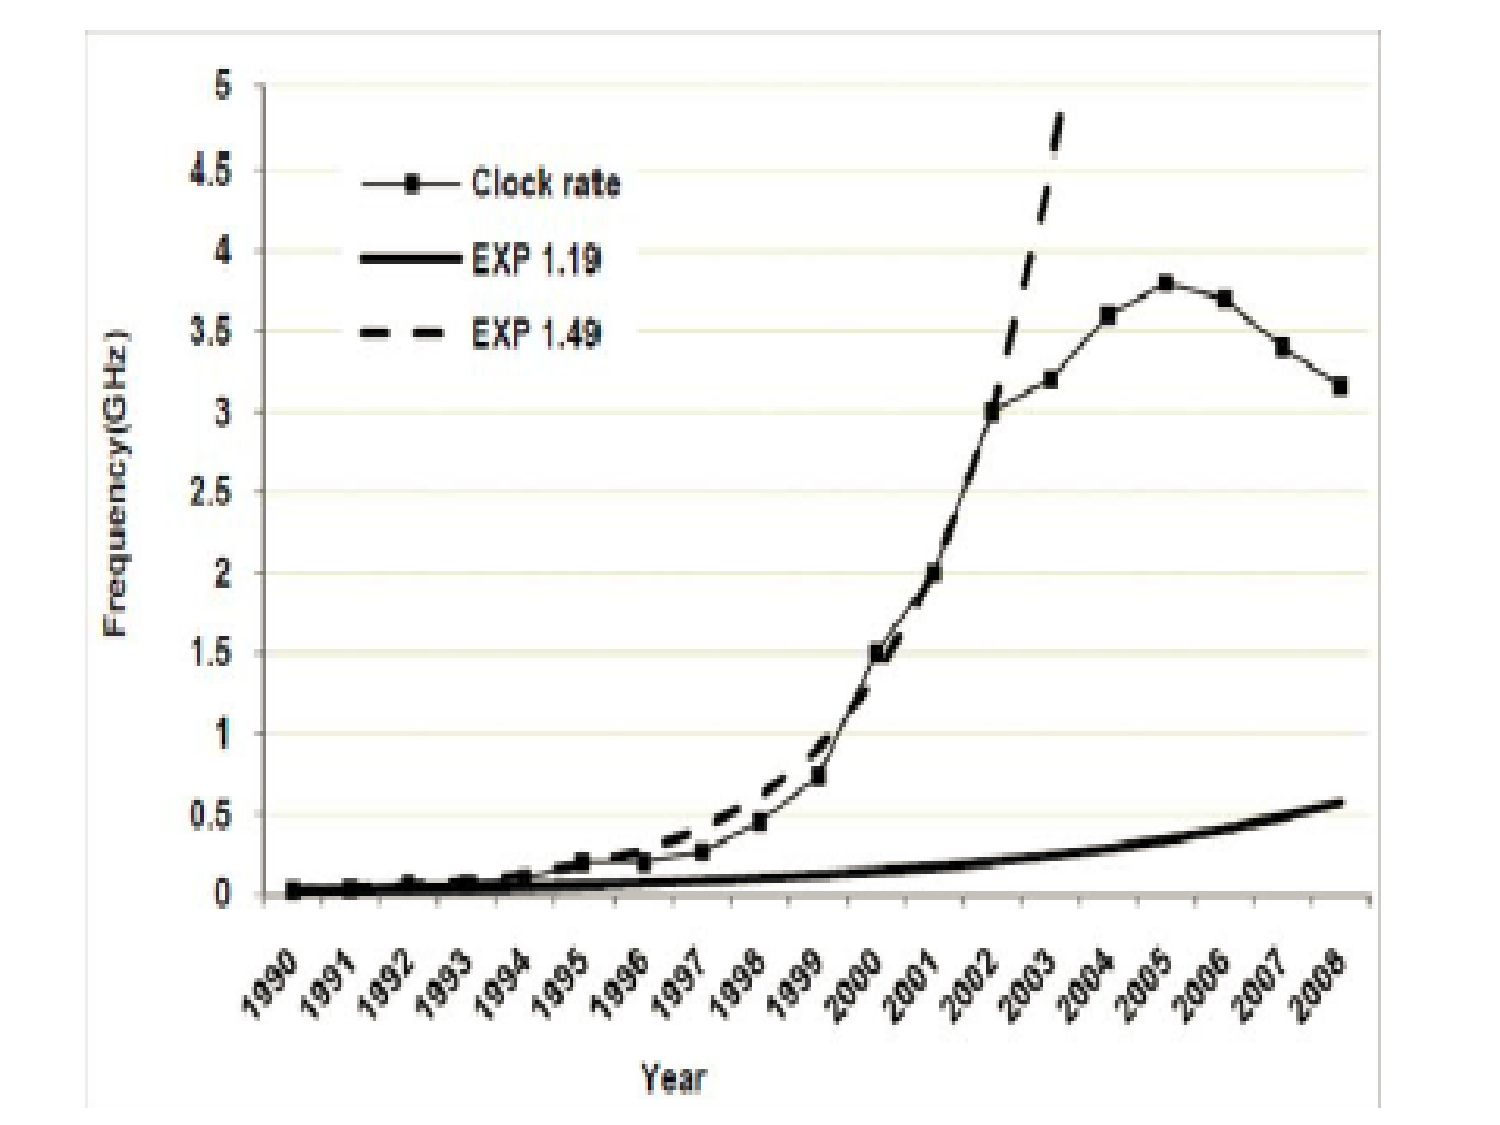
\includegraphics[width=70ex]{Figures/L1/FreqGraph}
\caption{Processor's Clock Frequency (Rate) between 1990-2008.}
%         The $y$ axis is 
%         the frequency; the $x$ axis is the time (years between 
%         1990-2008).}
\label{fig:cpu-freq}
\end{figure} 

Figure~\ref{fig:cpu-freq} shows that historically, the clock
rate (frequency) at which instructions are executed has
increased exponentially between $1990$ to $2004$.

The bolded line in the figure depicts an uniform increase of
$1.19\times$ per year, the dotted line depicts an increase of
$1.49\times$ per year, and the continuous line marked with
black rectangles depicts the actual increase in the clock rate.

The $1.19$ exponential corresponds to technology scaling:
the same hardware is being built on new technology. As silicon
technology improves, the distances shrink (a.k.a., process 
shrinking).  A new technology generation happens about
once every two years, and in each generation transistors'
switching speed increases about $41\%$, which directly
translates to an increase in the clock rate.

Between the years $1990-2002$ the actual increase in clock
rate has matched the $1.49$ exponential: clock rate has doubled 
every $21$ months. If that trend would have continued, we
would have had processors running at $30$GHz by 2008!

The difference between the $1.49$ and $1.19$ exponentials
(up until $2002$) corresponds to improvements in the processor
design. Examples include:
\begin{itemize}
    \item[(1)] Designing very-deep pipelines, consisting of $10-20$ stages.
            Having more stages in the pipeline means that each stage
            is less complex and thus it requires a smaller number of gates 
            per stage. 
            This means that the execution of a stage is quicker, which allows 
            to increase the clock rate. Historically, the number of
            gate delays has dropped by $25\%$ every process generation. 

    \item[(2)] aggressively exploiting instruction-level parallelism (ILP), 
            for example by means of out-of-order, speculative execution, 
            which combine techniques such as register renaming, reordering
            buffers, branch predication, lockup-free caches, speculative 
            memory disambiguation.

    \item[(3)] improvements in circuit design.
\end{itemize}

In $2004$, Intel cancels the design of the Pentium4 $@4$Ghz, and
switches track to multi-core design. This moment constitutes a 
tectonic shift away from the muscled deeply-pipelined uniprocessor.
The clock rate peaked in $2005$ but has mostly stalled since $2002$.

In essence, further increase of the clock rate is unsustainable 
because of a number of reasons: 
\begin{itemize}
\item First, it is unfeasible to build deeper pipelines because it is
difficult to imagine useful stages that can be built from less than
$10$ gates (we have already reached that point).

\item Second, the impact of technology scaling will be blunted in the
future due to wire delays, which do not scale, because the speed 
of wire transmission grows much slower than the switching speed.

\item Finally, and perhaps most importantly, circuits clocked at higher 
rates consume more power, and we have already reached the limits of
power consumption in single-chip microprocessors.
\end{itemize}

However, it is still the case that each process generation---which
roughly happens every two years---offers an additional budget of 
resources, such as transistors, that can be utilized to increase 
performance in other ways than sustaining clock-rate increases.
Figure~\ref{fig:feature-size} shows historical data related to how 
fast the feature size---a unit proportional to the gate length---has 
shrunk over the years and how fast the number of transistors have
grown. In essence, every two years we have a new process generation,
in which the feature size is reduced by about $30\%$ every generation.
The number of transistors also seems to double every two years 
(according to Moore's law), reaching one billion in $2008$.


\begin{figure}
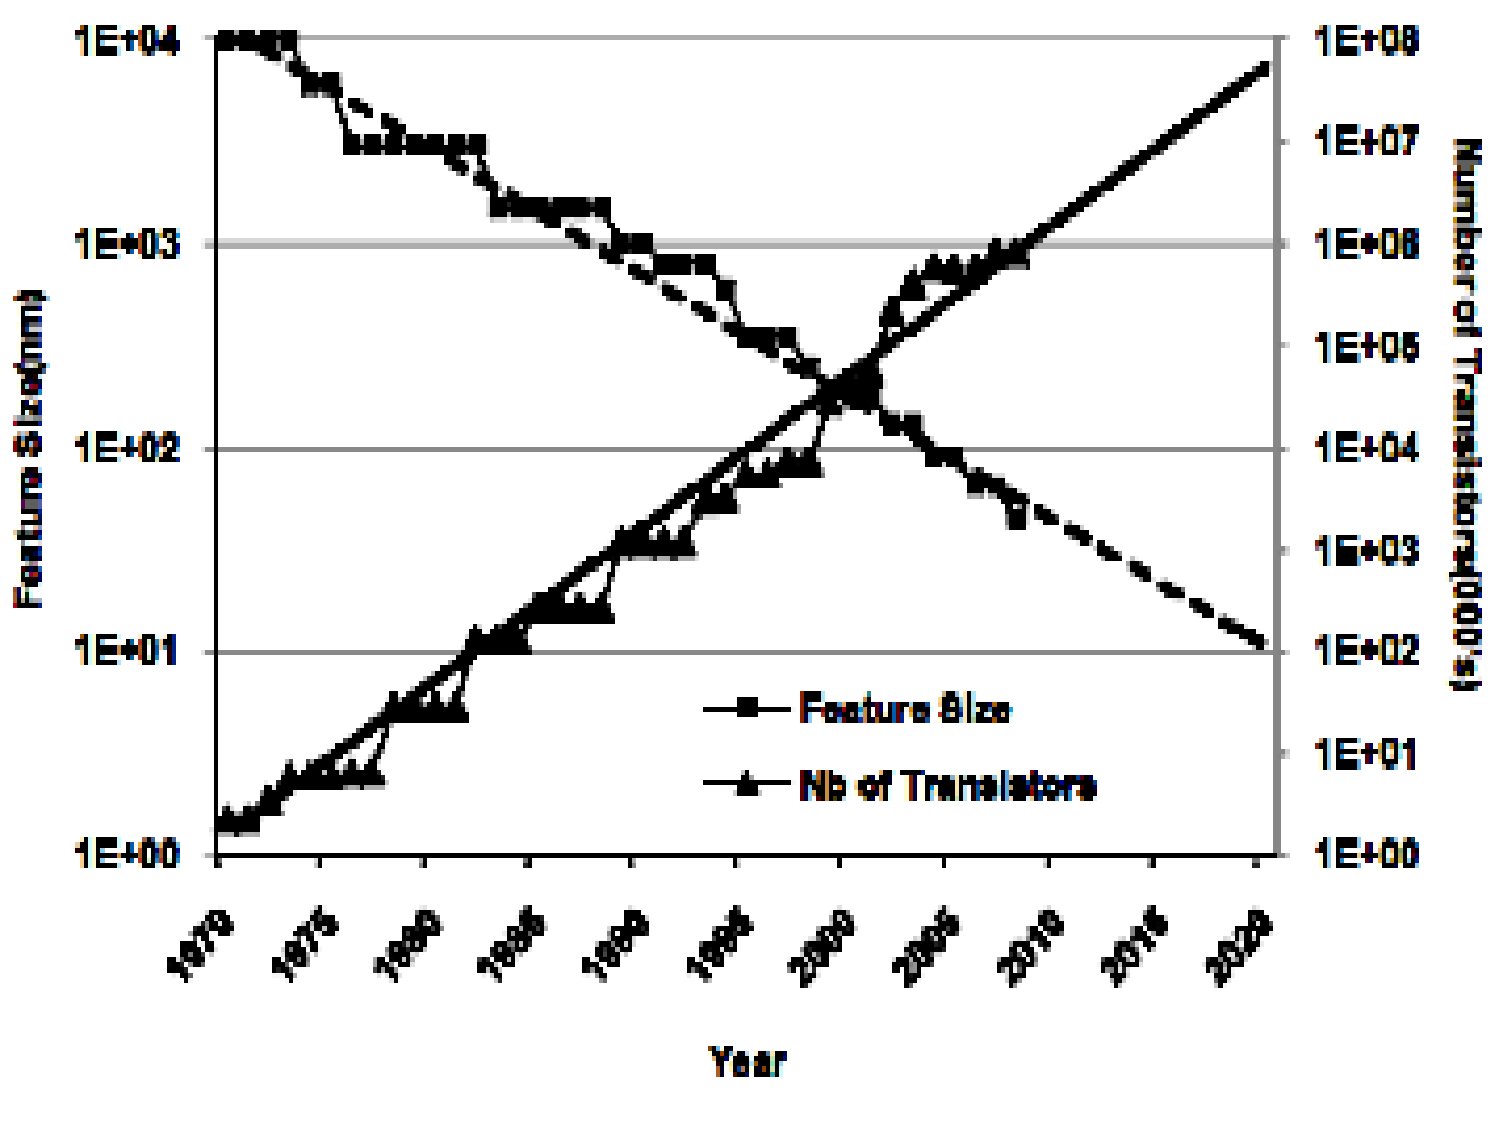
\includegraphics[width=90ex]{Figures/L1/FeatureSize} 
\caption{Historical data and prediction related to the feature-size 
         shrinkage and the number of transistors increase. The feature 
         size is shown by the line starting in the top-left corner;
         the number of transistors is shown in the line starting in 
         the bottom-left corner.}
\label{fig:feature-size}
\end{figure} 

The question thus becomes how to best utilize these hundreds of
billion of transistors in the quest for ever higher performance.
The design of highly-parallel hardware is one (if not the only)
viable direction in this sense. For example the budget of 
transistors can be used to:
\begin{itemize}
    \item enhance the parallelism of the memory system,
    \item to fetch and decode multiple instructions per clock,
    \item to run concurrently multiple hardware threads per 
            core, for example in order to hide the (high) latency
            of the memory system,
    \item to support thousands of cores that run threads in 
            parallel on different cores.
\end{itemize}

\subsection{Memory Wall! Which Memory Wall?}

The term ``memory wall'' was coined to denoted the seemingly
ever-growing gap between the processor and memory speed. This
wall is important because no matter how fast the processor is, 
it still needs to wait for the memory system to deliver the 
data to be processed. 

The historical trends related to memory have been that DRAM density 
increases $4\times$ every three years, but DRAM speed increases
only $7\%$ every year. This in comparison to the processor speed
increasing for a long time by $50\%$ per year.

\begin{figure}
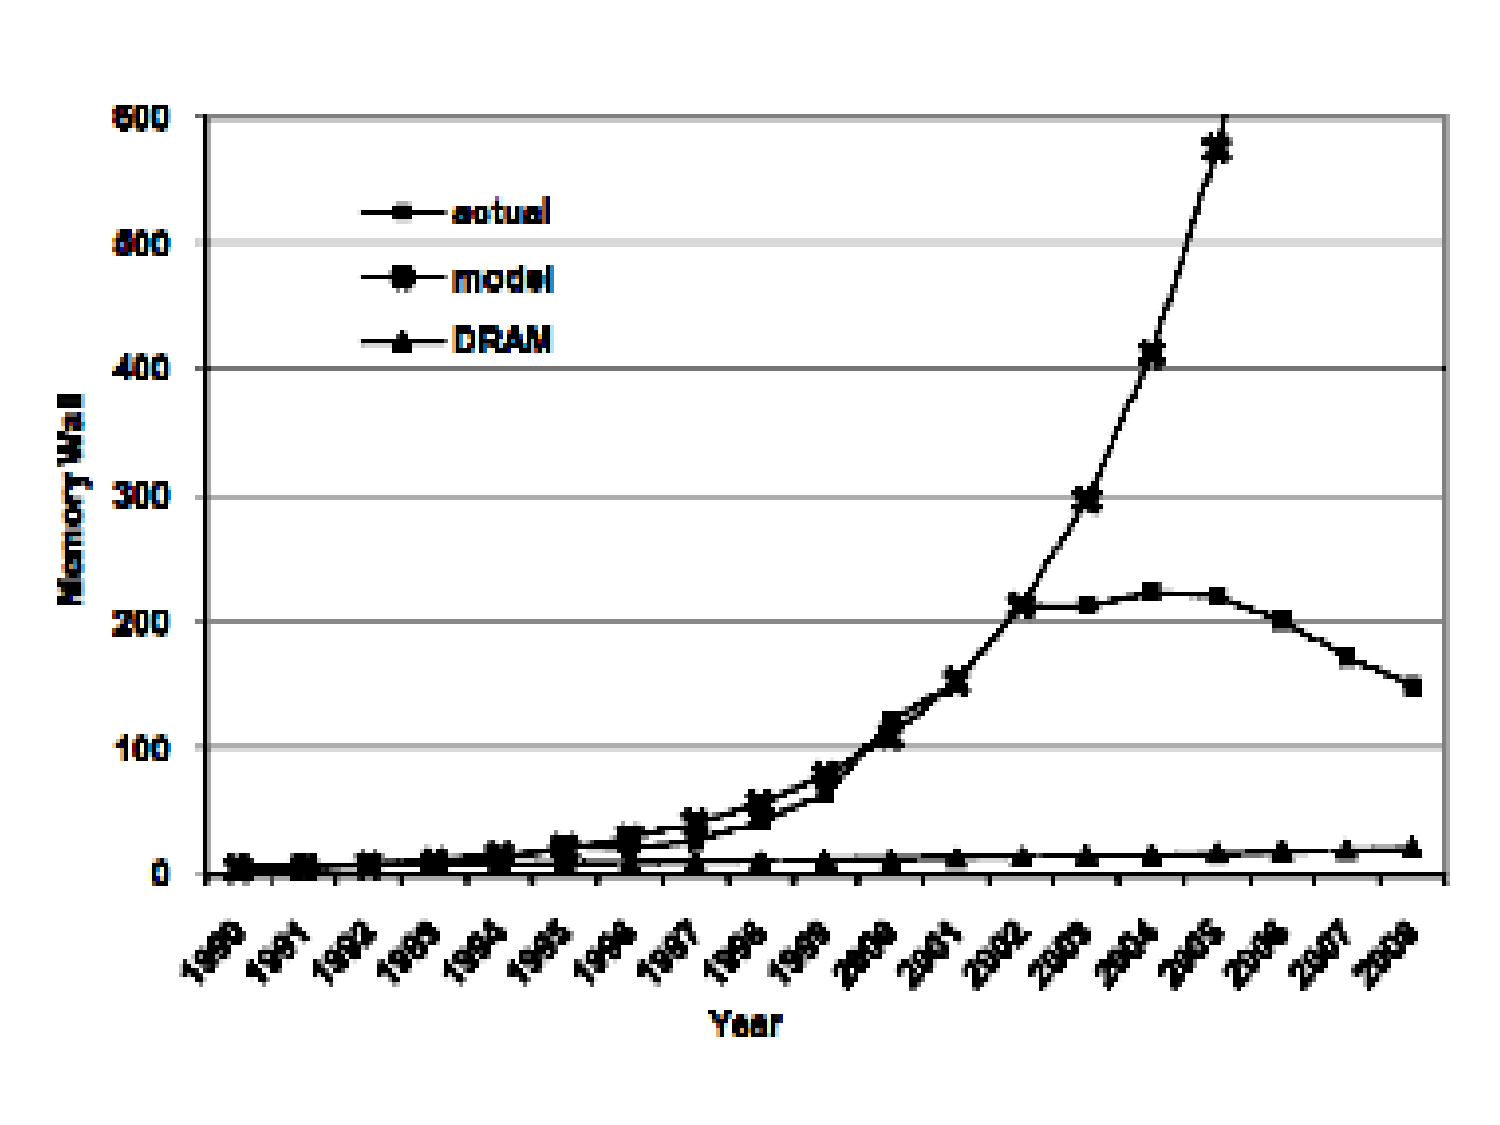
\includegraphics[width=90ex]{Figures/L1/MemWall}
\caption{Historical data related to the memory wall.}
\label{fig:mem-wall}
\end{figure} 

Figure~\ref{fig:mem-wall} shows the historical data related to
the memory wall, which is defined as the ratio between the memory
cycle and the processor cycle: In $1990$, the memory wall was about
$4$, i.e., the processor was running at about $25$MHz, while the 
memory cycle took about $150$ nanoseconds. (Since $1$Hz is $1$ 
cycle/sec, then the processor cycle was about $40$ nanoseconds.)

The memory wall has grown exponentially until $2002$, when it
reached $200$, and the perception was that the memory wall was 
going to last/grow forever.   However, it has stopped growing 
and actually has declined since $2004$ because the clock rate 
of the uniprocessor could not be increased anymore, while the 
DRAM speed still grows, albeit slower.   

As such, the advent of multi- and many-core systems have rendered 
the memory wall obsolete, but have introduced instead a bandwidth wall.
This is because nowadays, the memory subsystem needs to efficiently
feed cores that execute threads in parallel, which means that the
memory system has to be capable of delivering multiple data in 
the same time, which is measured by bandwidth.

%Unrelated, if the trend in DRAM-density increases continues 
%($4\times$ every three years), the figure predicts that DRAM memory 
%will reach one terabit by $2021$, which is still possible to happen.

\subsection{Technological Constraints}

In the past, the main trade-off related to architecture 
design has been between cost (area) and time (performance).
%
Today, the architectural design is challenged by several 
technological limits, such as power, wire delays, reliability,
complexity of design.  We will briefly examined each of them
in the following (sub)sections, and would conclude that 
parallel architectures seem to address well all these 
constraints.

\subsubsection{Power}
$\mbox{ }\\$
The major new constraint is power consumption, which is the sum of
dynamic and static powers:
\[ \mbox{\tt Total Power} ~=~ P_{dynamic} ~+~ P_{static}
\]
The dynamic power is consumed every time a gate is switching states,
i.e., from $0$ to $1$ or from $1$ to $0$, hence it is mostly dissipated 
in processors. It can be computed by the formula:
\[
P_{dynamic} ~=~ \alpha ~C ~V^2 ~f
\]
where $V$ denotes the supply voltage, $f$ denotes the clock rate, 
$T$ denotes the temperature, and $\alpha$ denotes the activity factor
(i.e., $\alpha f$ is the rate at which the gates switch).
%
In a given circuit, an increase in frequency requires a proportional
increase in the supply voltage as well, and a decrease in frequency
allows similarly to reduce the supply voltage. It follows that the
dynamic power consumed is roughly proportional to the cubic power
of the frequency, i.e., $P_{dynamic} \sim f^3$. 
%
As such, dynamic power consumption clearly favors parallel processing 
over increasing the clock rate of the uniprocessor. For example, 
increasing the frequency by a factor of $4\times$ consumes 
$4^3 = 64\times$ more dynamic power, but replicating a uniprocessor 
running at the original frequency $4$ times consumes only 
$4\times$ more dynamic power.
 


The static (leakage) power is dissipated in all circuits, at all times,
no matter of frequency and whether the circuit switches or not. 
In practice, it is dominated by cache leakage. It can be computed
with the formula:
\[
P_{static} ~=~ V ~I_{sub} ~\sim~ V ~e^{-k V_T / T}
\]
where $V_T$ denotes the threshold voltage---the voltage at which
a transistor switches off.  One can observe that the leakage power
increases exponentially as $V_T$ is reduced and as $T$ is increased.

The leakage power was negligible $15$ years ago, but since the feature 
size and the threshold voltage decreases with every process generation,
the leakage is getting worse. Currently, the leakage power has overtaken
dynamic power as the major source of dissipation. 

\subsubsection{Reliability}
$\mbox{ }\\$
Hardware errors/failures can be classified into several categories:
\begin{itemize}
    \item {\bf Transient Failures (Soft Errors).} The charge stored
        in a transistor is $Q = C ~ V$, where $C$ is the capacitance
and $V$ is the supply voltage. In every process generation the supply
voltage is reduced in order to maintain the electrical field at a 
constant strength. Thus $Q$ is considerable reduced at every process
generation, which results in every bit of storage in caches and 
processors being more prone to flip bits due to various corruption
sources, such as cosmic rays, alpha particles radiating from
the packaging material, electrical noise. In essence, the device
is operational, but the data has been partly corrupted. To protect
against such faults, DRAM/SRAM provide some form of error detection 
and correction capabilities.

    \item {\bf Intermittent/Temporary Failures} occur due to environmental
    variations on the chip, such as high temperature (hot spots). 
    In order for the device to return to correct behavior, the cause of
    the errors needs to be removed; for example the device should be 
    switched off for a while, so that the temperature drops. It follows
    that temporary failures last longer than transient failures, but
    they still allow to continue execution (by temporarily switching 
    off the faulty device).

    \item {\bf Permanent Failures} result in permanent damage to the device,
    which will never function properly ever again, and thus the device must 
    be isolated and replaced by a spare one.

\end{itemize}  

Chip mutiprocessors promote better reliability than uniprocessor systems:
For example, threads can be used to redundantly perform the same computation,
and a voting mechanism can be employed to decide the correct answer, and
to temporarily disable a core/resource. Similarly, faulty cores can be
detected and disabled automatically, while the remaining system remains
functional, albeit at a reduced capacity. This allows a natural failsafe
degradation of the system. 

\subsubsection{Wire Delays}
$\mbox{ }\\$
Each process generation shrinks distances, thus enhancing
miniaturization. The consequence is that transistors switch faster,
but the propagation of signals on wire does not keep pace with this
scaling.

To understand why this happens we take a look at the underlying 
physics. The propagation delay on a wire is proportional with the 
product between its resistance and capacitance $\sim R C$. 
The resistance, at its turn, is proportional with the ratio between 
the length and the cross-section area of the wire, i.e., 
$R \sim L / CS_{area}$.
The length of the wire shrinks with every process generation due 
to miniaturization; that is good! The problem however is that
the cross-section area shrinks as well due to the same reason,
which annuls much of the length-shrinking benefits.

The impact of wire delays also favors multiprocessors, because
communication traffic is hierarchical: most communication is 
local, while inter-core communication only happens occasionally.

\subsubsection{Design Complexity}
$\mbox{ }\\$
Design verification has become the dominant cost of chip
development today, and thus constitutes a major design constraint.
The principal reason is that chip density increases much faster 
than the productivity of verification engineers. Much like in
the case of software, this is due to the lack of new, high-level, 
productivity-oriented tools that also run fast.  Verification
is required at several levels of hardware design, such as:
\begin{itemize}
    \item at the gate and register-transfer language level: 
            verifying that the logic is correct,
    \item at the core level: verifying the correctness of 
            forwarding and memory-disambiguation protocols,
    \item at multicore level: verifying the cache-coherency
            and memory-consistency protocols.
\end{itemize}

To some extent, these verification difficulties have resulted in
dedicating the vast majority of chip resources to storage, simply
because it is trivial to increase the size of caches, store/reorder 
buffers, load/store/fetch queues, etc., without compromising the
safety of the design.

The design complexity trend also favors multiprocessors, as it is 
much easier to replicate the same structure multiple times than 
it is to design a large and complex system (or to bring improvements 
to one such). Similar to the case of storage, scaling up the
number of cores of a multiprocessor should not raise major
problems from a design perspective because, for example, 
any reasonable design of the cache-coherency infrastructure
should be parametric in the number of cores. 

\subsubsection{CMOS Meets Quantum Physics}
$\mbox{ }\\$
CMOS\footnote{
    Complementary metal-oxide semiconductor, abbreviated as CMOS,
    is the (current) technology used for constructing integrating 
    circuits. 
} is rapidly reaching the limits of miniaturization: if the current
trend continues, the feature size---defined as half the distance
between two metal wires---will be less than $10$ nanometers 
by year $2020$. This means that the gate length, which is about 
half the feature size, would be in the range of $5$ nanometers.

The radius of the atom is between $0.1$ and $0.2$ nanometers,
and is not affected at all by the miniaturization trends.
%
In essence, the gate length is quickly reaching the range of
atomic distances, which are governed by quantum physics, where
binary logic is replaced with probabilistic states.

While quantum computers are an area of active research, 
it is probably safe to say that commodity quantum hardware is 
not yet quite visible at the horizon. Until that time comes, 
the ever increase in compute power will be achieved by means 
of parallel architectures, such as (clusters of) many cores.
And even if/when quantum hardware will emerge as a viable 
technology, it is also clear that quantum software will be 
massively parallel by nature, so that at least the principles 
of parallel programming will remain of interest.

\newpage

\section{List Homomorphism (LH)}
\label{sec:ListHom}

The goal of the software track of PMPH is to teach the student 
how to ``think parallel''. To achieve this goal we start by
introducing in this section a very simple programming model, 
which utilizes only flat \lstinline{map}-\lstinline{reduce} 
operators, and which is rooted in the mathematical structure 
of list homomorphisms.

\subsection{Math Preliminaries: Monoid and Homomorphism}

This subsection briefly recalls the mathematical structures of
monoid and homomorphism.

A monoid is a set tupled with an associative binary operator, which
accepts an identity element within the set, and a group is a monoid
in which any element is invertible. In formal notation:

\begin{mydef}[Monoid]\label{MonoidDef}
$\mbox{ }$\\
Assume a set $S$ and a binary operator $\odot : S \times S \rightarrow S$.\\
\emph{$(S, \odot)$ is called a monoid} if it satisfies the following two axioms:\\
\emph{(1) Associativity:} $\forall x,y,z\in S$ we have 
    $(x \odot y) \odot z \equiv x \odot (y \odot z)$ and\\
\emph{(2) Identity Element:} $\exists e \in S$ such that $\forall a \in S$, %we have
    $e \odot a \equiv a \odot e \equiv a$.\\\medskip
\end{mydef}

\begin{mydef}[Group]\label{GroupDef}
$\mbox{ }$\\
$(S,\odot)$ is called a group if it is a monoid satisfying the additional
property that any element is  invertible:\\ 
    $\forall a, ~\exists a^{-1}$ such that 
    $a\odot a^{-1}\equiv a^{-1}\odot a\equiv e$.
\end{mydef}

For example, 
\begin{itemize}
    \item $(\mathbb{Z},+)$ denotes the monoid formed by the set of (signed) 
            integers with the addition operation, which has $0$ as neutral
            element. $(\mathbb{Z},+)$ is also a group because any integer
            $i$ has an inverse $-i$, which also belongs to $\mathbb{Z}$. 
            is a group with neutral element $0$.
    \item $(\mathbb{N},+)$ denotes the monoid of natural numbers with
            addition, which has $0$ as neutral element. $(\mathbb{N},+)$  
            is not a group because for example $1$ does not have an 
            inverse in $\mathbb{N}$.
    \item $(\mathbb{Z},\times)$ is the monoid of integers with multiplication,
            which has $1$ as neutral element. $(\mathbb{Z},\times)$ is not
            a group because for example $2$ is not invertible in $\mathbb{Z}$.
            ($\frac{1}{2} \not\in \mathbb{Z}$)
    \item $(\mathbb{L}_T,++)$, is the monoid formed by the set of lists of 
            elements of some type $T$ ($\mathbb{L}_T$), together with the
            list concatenation operator ($++$), which has the empty list
            ($[]$) as neutral element.   $(\mathbb{L}_T,++)$ is obviously
            not a group.
\end{itemize}

A monoid homomorphism is a function between two monoids, such that 
operations on one monoid can be directly mapped into operations on
the second monoid. In formal notation:  

\begin{mydef}[Monoid Homomorphism]\label{HomDef}
$\mbox{ }$\\
\emph{A monoid homomorphism} from monoid $(S,\oplus)$ to monoid $(T,\odot)$
is a function $h : S \rightarrow T$ such that $\forall u, v\in S$,
\emph{$h(u\oplus v) \equiv h(u)\odot h(v)$}.
\end{mydef}


\subsection{The Shape of a List-Homomorphic Function/Implementation}

Throughout this chapter, we will work with finite lists,
albeit the gained insight will carry over to arrays, which
is the main datatype promoting efficient execution on 
modern hardware. We recall that $(\mathbb{L}_T,++)$ is
a monoid:
\begin{itemize}
    \item {\tt ++} denotes list concatenation, for example\\
    {\tt [1, 2, 3] ++ [4, 5, 6, 7] $\equiv$ [1, 2, 3, 4, 5, 6, 7]}
    \item {\tt []} denotes the empty list, which is the neutral 
          element for concatenation:\\ 
            $\forall$ list {\tt x}, we have that 
            {\tt [] ++ x $\equiv$ x ++ [] $\equiv$ x}
\end{itemize}

We will use the term \emph{list-homomorphic function} (LHF)
to denote a function, which accepts an implementation (LHI)
that uses a certain form of divide and conquer programming, 
as defined below.
 
\begin{mydef}[List-Homomorphic Function/Implementation LHF/LHI]\label{LH-FI-Def}
$\mbox{ }$\\
A LHF function $h$ is a (mathematical) function that can be implemented as: 
\begin{lstlisting}[mathescape=true]
h( [ ] )   = e
h( [x] )   = f(x)
h( x ++ y) = h(x) $\odot$ h(y)
\end{lstlisting}
%and which always computes the same result no matter on how 
%the input list is partitioned into {\tt x ++ y}.
\end{mydef}\vspace{-2ex}

In simple words a LH implementation consists of:
\begin{itemize}
    \item[(1)] A divide-and-conquer case 
            {\tt h( x ++ y) = h(x) $\odot$ h(y)},
            which allows to partition the input list {\tt z} 
            into any two sublists {\tt x} and {\tt y} such that
            {\tt z = x ++ y} and the implementation
            applies recursively {\tt h} to the sublists and 
            combines the results with the operator $\odot$.   
            We draw attention to the following important observations:
        \begin{itemize}
            \item[(a)] in order for $h$ to be well defined as a mathematical 
            function (i.e., for the implementation to be useful in practice), 
            $h$ needs to compute the same result no matter of how the input 
            list is partitioned into {\tt x} and {\tt y}. This is an implicit 
            assumption.

            \item[(b)] {\tt h( x ++ y) = h(x) $\odot$ h(y)} essentially
            defines a homomorphism between the monoid $(\mathbb{L}_T,++)$ 
            and another monoid $(Img(h),\odot)$ whose set is the
            image\footnote{
                The image of a function $f : A \rightarrow B$ is the
                subset of $B$ covered by the application of $f$ to
                all elements of $A$.
            } of {\tt h} and its binary operator is $\odot$.
            One remaining question is: ``who is the neutral element of 
            $(Img(h),\odot)$?''
        \end{itemize}

    \item[(2)] Two base cases corresponding to {\tt h} being applied to 
                the empty list and to a list formed by exactly one element:
        \begin{itemize}

            \item[(a)] {\tt e} is the implementation of the
                empty-list case, i.e., {\tt h( [ ] ) = e} and  
                it is actually and provably the neutral element of $(Img(h),\odot)$.
            \item[(b)] the other base case is implemented as
                the application of a function {\tt f} to the
                (single) element of the list.
        \end{itemize}
\end{itemize}

The LHI implementation is utterly unsuitable to being mapped efficiently
to modern highly-parallel hardware, for example because GPUs\footnote{
We use GPU as the abbreviation for general-purpose graphical processing
units.} do not support recursion. However, we remark that the function 
{\tt f}, the binary operator $\odot$ and the neutral element {\tt e} 
are explicitly provided by the LHI and they will allow us later to 
straightforwardly translate this LHI to another implementation which 
can be efficiently mapped on GPU hardware.

The following theorem summarizes our previous observations:
\begin{mytheo}[LHF is a Mathematical Homomorphism]\label{LHF-as-Hom}
$\mbox{ }$\\
A list-homomorphic function (which computes the same result
regardless of how the list is partitioned):
\begin{lstlisting}[mathescape=true]
h( [ ] )   = e
h( [x] )   = f(x)
h( x ++ y) = h(x) $\odot$ h(y)
\end{lstlisting}\vspace{-2ex}
is a mathematical homomorphism from $(\mathbb{L}_T,++)$ to $(Img(h),\odot)$.\\
In particular $(Img(h),\odot)$ must be a monoid with neutral element {\tt e},
which also means that $\odot$ must be associative.\smallskip

The reverse also (trivially) holds: if {\tt h} is a homomorphism between
$(\mathbb{L}_T,++)$ and some monoid $(M,\odot)$ then it accepts a LHI
(as above).\\
\emph{The proof} is left as an exercise. 
\end{mytheo}

\subsection{Examples of List-Homomorphic Implementations}
\label{subsec:LH-egs}

We have discussed so far list homomorphism at a rather abstract
level. This section aims at demonstrating that list-homomorphism
programming is actually quite natural (when it fits) by examining 
several simple code examples. The examples use a notation that 
somewhat resembles Haskell, for example
\begin{itemize}
    \item  greeks such as $\alpha$ denote arbitrary types (type variable),
      and $[\alpha]$ denotes the type of a list whose elements are
      of type $\alpha$,
       
    \item \lstinline{f a b} applies the function \lstinline{f} to two arguments 
      \lstinline{a} and \lstinline{b}, 

    \item \lstinline{&&}, \lstinline{||} correspond to logical and, or operators. 
\end{itemize}

We discuss the following examples:
\begin{itemize}
\item[len:] The first example corresponds to computing the
                length of a list, i.e., 
                {\tt len : $[\alpha] ~\rightarrow$ Int}.
                %The LHI could be:
\begin{lstlisting}[mathescape=true]
len [ ] = 0
len [x] = one x -- where one x = 1
len (x ++ y) = (len x) + (len y)
\end{lstlisting}\vspace{-2ex}
            The first base case says that an empty list has size $0$.
            The second base case says that a list containing exactly
            one element has size $1$; however the LHI form requires
            to call a function on the list's single element, so we
            have defined the function \lstinline{one} to always return $1$
            no matter the argument.
            Finally, the divide-and-conquer case says that if we
            partition the input list into two sublists then the length
            of the initial list is the sum of the lengths of the
            two sublists.\medskip

\item[all$_p$:] The second example corresponds to the function {\tt all$_p$}
            that checks whether some predicate {\tt p : $\alpha ~\rightarrow$ Bool}
            satisfies (holds on) all elements of an input list:
\begin{lstlisting}[mathescape=true]
all$_p$ [ ]      = true
all$_p$ [x]      = p x
all$_p$ (x ++ y) = (all$_p$ x) && (all$_p$ y)   
\end{lstlisting}\vspace{-2ex}
            The base cases say that an empty list satisfies the
            predicate (why?) and that a list containing exactly
            one element satisfies the predicate if and only if
            the element satisfies the predicate (obviously). 
            The recursive, divide and conquer case says that
            a predicate satisfies a list (\lstinline{z = x ++ y}) 
            if and only if it it satisfies both (sub)partitions 
            {\tt x} and {\tt y}.
            The implementation of the empty-list case must be
            \lstinline{true} because this is the neutral element of
            the monoid form by the two-element set 
            {\tt $\{$true, false$\}$} and the logical-and operator (\lstinline{&&}).
            Further intuitive confirmation is given by the fact
            that if {\tt all$_p$ []} is chosen \lstinline{false}
            then the function {\tt all$_p$} is ill-defined,
            in that it can generate two different results for the same
            input. For example, assume \lstinline{p x = x > 3}. Then 
            {\tt all$_p$ [5, 6]} should result in \lstinline{true}
            because all its elements are greater than three. However,
            the following legal derivation produces \lstinline{false}:
\begin{lstlisting}[mathescape=true]
all$_p$ [5, 6] $\equiv$ all$_p$ ([] ++ [5, 6]) $\equiv$ (all$_p$ []) && (all$_p$ [5, 6]) $\equiv$ 
false && (all$_p$ [5, 6]) $\equiv$ false.
\end{lstlisting}

\item[sum:] The third example corresponds to summing up the (numerical) elements
            of a list. Without further explanation, this can be accomplished
            with the following LHI:
\begin{lstlisting}[mathescape=true]
sum [ ]      = 0
sum [x]      = id x -- where id x = x
sum (x ++ y) = (sum x) + (sum y)
\end{lstlisting}\vspace{-2ex}

\item[fld:] The fourth example corresponds to the function that adds two
            to every (numeric) element of a list and then multiplies the results.
            In F\# this can be expressed as\\ 
            \lstinline{fold (\acc x -> acc * (x+2)) 1 mylist}\\
            Without further ado, this can be accomplished with the following LHI:
\begin{lstlisting}[mathescape=true]
fld [ ]   = 1
fld [x]   = plus2 x -- where plus2 x = x + 2
fld (x ++ y) = (fld x) * (fld y)
\end{lstlisting}\vspace{-2ex}
\end{itemize} 


\subsection{Map, Reduce and List Homomorphism Theorems}

This section (i) starts by introducing two of the (three) important 
basic blocks that lay the foundation of data-parallel programming
(\lstinline{map} and \lstinline{reduce}),
then (ii) presents the first theorem of list homomorphism, which 
basically gives a straightforward way of translating a LHI into
a semantically-equivalent \lstinline{map-reduce} implementation,
and (iii) it concludes by presenting several other theorems that
can be seen as simple re-write rules that allow to optimize the 
program in various ways.

It is perhaps important to notice that while the discussion refers
to lists, this is only to preserve consistency with the
list-homomorphism presentation. List is an implicitly sequential 
datatype; whenever we mention lists from now on, the reader
should think arrays, at least in what parallel execution is concerned. 

The first basic-block of data parallel programming is the 
\lstinline{map} second-order operator, which takes as argument 
an unary function and a list of elements, and produces a list 
of the same length as the original one by applying the function 
argument to each element of the input list.  
The type and semantics of \lstinline{map} are presented below:
\begin{lstlisting}[mathescape=true]
map : $(\alpha \rightarrow \beta) ~\rightarrow ~[\alpha] ~\rightarrow~ [\beta]$
map f [x$_1,\ldots$x$_n$] = [f x$_1$,$\ldots$, f x$_n$]
\end{lstlisting}\vspace{-2ex}

Please note that, assuming a pure-functional language and replacing
lists with arrays, \lstinline{map} has implicitly parallel semantics, 
because the computation corresponding to some element {\tt x$_i$}
of the array is completely independent of the computations of all
other elements of the array.


The second basic-block of data parallel programming is the
\lstinline{reduce} second-order operator, which takes as arguments
an \emph{associative} binary operator, the neutral element corresponding
to the monoid defined by the binary operator, and a list of elements.
The result of \lstinline{reduce} is obtained by successively applying 
the operator to all the elements of the array. The type and semantics of 
\lstinline{reduce} are presented below:
\begin{lstlisting}[mathescape=true]
reduce : $(\alpha \rightarrow \alpha \rightarrow \alpha) ~\rightarrow~ \alpha ~\rightarrow~ [\alpha]~ \rightarrow \alpha$
reduce $\odot$ e [x$_1,\ldots$x$_n$] = e $\odot$ x$_1$ $\odot~\ldots~\odot$ x$_n$
\end{lstlisting}\vspace{-2ex}

Unlike \lstinline{map}, the parallel semantics of \lstinline{reduce}
is not straightforward to see. We demonstrate it in 
\cref{fig:reduction-tree}: assuming an infinite number of
processors, the parallel computation of \lstinline{reduce} is 
performed by means of a reduction tree, which performs sequentially
a number of {\tt log(n)} parallel operations, where we have denoted
by {\tt n} the length of the input array. 


\begin{figure}
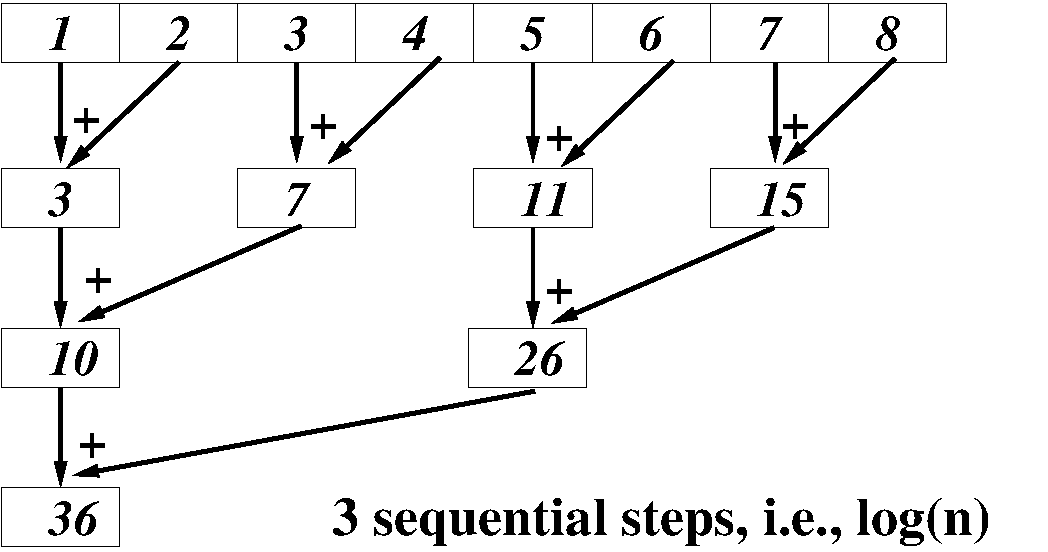
\includegraphics[width=70ex]{Figures/L1/ReduceEg.pdf}
\caption{Parallel execution of \lstinline{reduce} requires
        a sequence of \lstinline{log(n)} parallel operations
        ({\tt n} is the array length).}
\label{fig:reduction-tree}
\end{figure} 

It is perhaps important to stress (again) that $\odot$ \emph{\bf must be 
associative}:
\begin{itemize}
    \item In parenthesis, that is why we did not bother to put 
the parenthesis that would specify the execution order, 
but the commonly-used sequential implementation of \lstinline{reduce} 
accumulates to the left, i.e., 
{\tt ((e $\odot$ x$_1$) $\odot~\ldots~\odot$ x$_n$)}.

    \item More importantly, if $\odot$ is not associative then the 
    sequential and parallel execution of \lstinline{reduce} will likely
    give different results. For example,  assume the list \lstinline{[1,2,3,4]}
    which is reduced with the non-associative operator {\tt acc $\odot$ x = acc + 2*x}.
    Even ignoring the neutral element, sequential execution will 
    result in {\tt (((1 $\odot$ 2) $\odot$ 3) $\odot$ 4) = 19}
    and parallel execution will result in 
    {\tt (1 $\odot$ 2) $\odot$ (3 $\odot$ 4) = 5 $\odot$ 11 = 27},
    according to the execution patterns of the reduction tree shown
    in \cref{fig:reduction-tree}.
    
    \item It should be clear now that \lstinline{reduce} is different
        that \lstinline{fold} (from F\#). This can be seen from
        the type of {\tt fold : ($(\beta \rightarrow \alpha \rightarrow \beta) ~\rightarrow~ \beta ~\rightarrow~ [\alpha]~ \rightarrow \beta$}; in particular it does not make sense
        to talk about the associativity of \lstinline{fold}'s operator
        because of the wrong type---associativity makes sense on
        binary operators whose arguments and result have the same type.
        Moreover, even when the type happens to be correct, as in the
        previously-discussed case, we have still seen that \lstinline{fold} 
        is not a parallel operator because it does not require associativity.
        In particular \lstinline{fold (\acc x -> acc + 2*x) 0 lst}
        can be parallelized by re-writing it as a \lstinline{map-reduce} 
        composition: \lstinline{reduce (+) 0 (map (+2) lst)}!

    \item In practice forgetting that the \lstinline{reduce} operator
             must be associative---i.e., using \lstinline{reduce} with
             non-associative operators---is one of the main generators 
             of difficult-to-find bugs.
\end{itemize}

Similarly, remember that {\tt e} must be the neutral element of the 
monoid defined by $\odot$---hence reducing an empty list results in 
{\tt e}, and {\tt e} can be safely omitted from the computation if 
the list is not empty (because by the definition of the neutral 
element, we have that {\tt e $\odot$ x $\equiv$ x, $\forall$ x}).

\subsubsection{First List-Homomorphism Theorem}
$\mbox{ }$\\

The first LH theorem~\cite{ThirdLHTh} basically gives a 
straightforward way of rewriting a LHI as a \lstinline{map-reduce} 
composition, as stated in the theorem below, which uses $\circ$ 
to denote the function-composition operator.

\begin{mytheo}[1$^{st}$ LH Theorem]\label{1st-LH-TH}
$\mbox{ }$\\
A list-homomorphic implementation defined as:
\begin{lstlisting}[mathescape=true]
h( [ ] )   = e
h( [x] )   = f(x)
h( x ++ y) = h(x) $\odot$ h(y)
\end{lstlisting}\vspace{-2ex}
is semantically equivalent with
(\lstinline{reduce}$~\odot~$\lstinline{e})$~~\circ~~$(\lstinline{map f}),
or in complete code:
\begin{lstlisting}[mathescape=true]
h z $\equiv$ reduce $\odot$ e (map f z)
\end{lstlisting}\vspace{-2ex}
\end{mytheo}

\cref{1st-LH-TH} also provides the theoretical argumentation of why the
\lstinline{reduce} operator must be associative: if $h$ is a list
homomorphism, then $(Img(h),\odot)$ must be a monoid, and by definition,
a monoid requires its operator $\odot$ to be associative.

Applying \cref{1st-LH-TH} to the LHI discussed in \cref{subsec:LH-egs}
results in the following \lstinline{map-reduce} implementations:
\begin{itemize}
    \item \lstinline{len z} $\equiv$ \lstinline{reduce (+) 0 (map one z)}
    \item {\tt all$_p$ z $\equiv$} \lstinline{reduce (&&) true (map p z)}
    \item \lstinline{sum z} $\equiv$ \lstinline{reduce (+) 0 (map id z)} $\equiv$ \lstinline{reduce (+) 0 z}
    \item \lstinline{fld z} $\equiv$ \lstinline{reduce (*) 1 (map plus2 z)}
\end{itemize}

We have thus started from an arguably natural program specification rooted 
in the mathematical theory of list homomorphisms, and we have translated
that into an implementation in which parallelism is made explicit by
\lstinline{map-reduce} operators and which can be straightforwardly
mapped to modern parallel architectures. We discuss simple program
optimizations next.

\subsubsection{Other List-Homomorphism Lemmas}

\begin{mytheo}[LH Promotion Lemmas]\label{LH-PROMS}
$\mbox{ }$\\
Given unary functions \lstinline{f} and \lstinline{g}, and an 
associative binary operator $\odot$ with neutral element {\tt e$_{\odot}$}
then the following three identities hold, where $\circ$ denotes 
function composition:\\
\begin{lstlisting}[mathescape=true]
1. (map f) $\circ$ (map g) $\equiv$ map (f $\circ$ g)
2. (map f) $\circ$ (reduce (++) []) $\equiv$ (reduce (++) []) $\circ$ (map (map f))
3. (reduce ($\odot$) e$_{\odot}$) $\circ$ (reduce (++) []) $\equiv$
                         (reduce ($\odot$) e$_\odot$) $\circ$ (map (reduce ($\odot$) e$_{\odot}$)) 
\end{lstlisting}
If you are unfamiliar with the functional notation for composition, 
the identities can be written in full as:\\
\begin{lstlisting}[mathescape=true]
1. map f (map g zs) $\equiv$ map ($\lambda$ z $\rightarrow$ f (g z)) zs
2. map f (reduce (++) [] zs) $\equiv$ reduce (++) [] (map ($\lambda$z$\rightarrow$map f z) zs)
3. reduce ($\odot$) e$_{\odot}$ (reduce (++) [] zs) $\equiv$ 
                        reduce $\odot$ e$_\odot$ (map ($\lambda$ z $\rightarrow$ reduce $\odot$ e$_{\odot}$ z) zs) 
\end{lstlisting}\vspace{-2ex}
\end{mytheo}

The identities can be seen as re-write rules that can be used
to optimize the program in various ways, for example:
\begin{itemize}
    \item[(1)] The first identity is known as the \lstinline{map} fusion/fission
        rule:
        \begin{itemize}
            \item[$\Rightarrow$] Fusion corresponds to applying the transformation 
                    in the forward ($\Rightarrow$) direction, and is 
                    useful for reducing the number of accesses to
                    global memory, which is very slow in comparison
                    with registers. For example, the left-hand side
                    program: \lstinline{let tmp = map g zs in map f tmp}
                    requires to read and write in the first \lstinline{map}
                    each element of arrays {\tt zs} and {\tt tmp}, respectively,
                    followed by reading and writing in the second 
                    \lstinline{map} each element of {\tt tmp} and result
                    arrays, respectively. This counts up to $4$ accesses
                    to global memory per element. The program on the
                    right-hand side: \lstinline{map (}$\lambda$ {\tt z} $\rightarrow$ {\tt f (g z)) zs} 
                    requires reading and writing the input and result arrays
                    only once, thus halving the number of accesses to global
                    memory per element---because the intermediate computation
                    {\tt g z} is hold in registers, not in memory.
            \item[$\Leftarrow$] Fission corresponds to applying the transformation 
                    in the backward ($\Leftarrow$) direction and is useful
                    for enhancing the degree of parallelism that is statically mapped
                    to hardware, in the context of a nested-parallel program.
                    (This will be discussed in detail later on in the context 
                    of the flattening transformation and vectorization.)
        \end{itemize}

    \item[(2,3)] Similar to fusion/fission, the second and third identities can 
                    be used in the forward 
                    direction ($\Rightarrow$) to efficiently sequentialize 
                    the parallelism in excess of what the hardware can support, 
                    and in the backward direction ($\Leftarrow$)  
                    to enhance load balancing and the program's degree of 
                    parallelism that can be statically mapped to hardware.
        \begin{itemize}
            \item[$\Rightarrow$]
                    Assume {\tt split$_p$} denotes the operator that splits a 
                    list into $p$ sublists of roughly equal lengths. Please 
                    observe that {\tt (reduce (++) []) $\circ$ split$_p$ $\equiv$ id},
                    meaning that splitting a list into $p$ sublists, then
                    flattening the resulted list results in the original list.
                    ({\tt id x = x} stands for the identity function.)
                    One may straightforwardly derive a new identity, presented
                    below by composing both sides of identity (2) with {\tt split$_p$}:
                    \begin{center}\lstinline{map f} $\equiv$ \lstinline{(reduce (++) [])} $\circ$ \lstinline{(map (map f))} $\circ$ {\tt split$_p$} (2')\end{center}
                    The difference is that (2) necessarily operates on lists, while 
                    (2') operates on list of lists.   We are interested in using 
                    this new identity in the forward ($\Rightarrow$) direction. 
                    Assume the hardware
                    has $p$ cores, and that the input list (array) contains
                    $n$ elements, where $n$ is much larger than $p$. The left-hand side 
                    \lstinline{map f} suggests an execution model that spawns $n$
                    threads---this is suboptimal on many architectures.
                    The translation basically aims to spawn a number of threads
                    equal to the number of cores. This is achieved by splitting
                    the list, then processing sequentially each chunk on one core
                    (by the inner \lstinline{map}), while processing the $p$ chunks 
                    in parallel (by the outer \lstinline{map}), and finally by
                    concatenating the per-core results. Similar thoughts apply to
                    the third identity.   
                    
            \item[$\Leftarrow$] Consider a program similar to the left-hand side
                    of the original identity $2$. Its input is necessarily a list
                    of lists. Assume the input list has $p$ unbalanced sublists, 
                    for example all sublist have $2$ elements, except for the
                    last one which has $n - 2\cdot p - 2$ elements, where 
                    $n$ is big. If executed as suggested by the right-hand side---each
                    core processes a sublist---the parallel execution will be
                    utterly unbalanced because the last core will process many
                    more items than the rest of the cores. If processing an
                    item uniformly takes one unit, then the speedup achieved 
                    by the right-hand side program will be $\frac{n}{n - 2 \cdot p - 2}$
                    which converges to $1$ when $n$ goes to infinity.
                    Instead, one can apply the second identity in the $\Leftarrow$ 
                    direction to flatten parallelism, then one can apply again 
                    the forward direction as in the $\Rightarrow$ bullet above
                    by splitting the concatenated list again into $p$ sublists 
                    of \emph{roughly-equal} lengths. The execution of the resulting
                    program is now load-balanced, each core processing a similar
                    number of elements, resulting in a speedup close(er) to
                    the optimal $p\times$. Similar thoughts apply to the third identity.
        \end{itemize}
\end{itemize}


The final theorem is often used for optimizing the scheduling of 
\lstinline{map-reduce} computations, for example in frameworks such
as OpenMP. The idea is that a \lstinline{map-reduce} composition
can be re-written into a semantically equivalent program that:
\begin{itemize}
    \item splits the input list into $p$ sublists of roughly
            equal length,
    \item applies the original computation to each sublist,
            such the computation of a sublist is performed
            sequentially on a core, but different sublists
            are processed in parallel on different cores, 
    \item applies the original reduction to the per-core
            results.
\end{itemize}
The benefit of such an execution is not only given by
spawning a number of threads equal to the numbers of cores,
thus reducing scheduling and switching-contexts overheads,
but also optimizing the reduction depth. Originally,
the reduction was applied to a list of $n$ elements,
and would require $log(n)$ sequential steps (see reduction
tree in \cref{fig:reduction-tree}). In the
transformed program the final (parallel) reduction
is performed on a list of $p$ elements, requiring only
$log(p)$ sequential steps.

\newpage
\begin{mytheo}[Optimized Map-Reduce Lemma]\label{Lemma-Map-Red}
Assume {\tt split$_p :: [\alpha] \rightarrow [[\alpha]]$}
distributes a list into $p$ sublists, each containing about 
the same number of elements. Also assume $\odot$ a binary 
associative operator with neutral element {\tt e$_{\odot}$} 
and {\tt f} a unary function. The following identity always holds:
\begin{lstlisting}[mathescape=true]
redomap ($\odot$) f e$_{\odot}$ $\equiv$
(reduce ($\odot$) e$_{\odot}$) $\circ$ (map (redomap ($\odot$) f e$_{\odot}$)) $\circ$ split$_p$
\end{lstlisting}\vspace{-2ex}

where \lstinline{redomap} is defined as
\lstinline{redomap} $\odot$ {\tt f e$_{\odot}$} $\equiv$ \lstinline{(reduce} $\odot$ {\tt e$_{\odot}$)} $\circ$ \lstinline{(map f)}.

\emph{The Proof} is left as an exercise. 
\end{mytheo}

In what the proof of \cref{Lemma-Map-Red} is concerned, the big hint is to first 
observe that\\
\lstinline{(reduce (++) [])} $\circ$  {\tt distr$_p$} results in the identity function,
which is the neutral element for function composition---concatenating the result obtained
by splitting an input list results in the input list. As such we can start
by composing the left-hand side with the identity written as before:\\
\lstinline{redomap} {\tt($\odot$)} {\tt f e$_{\odot}$} $\equiv$ \lstinline{(reduce} {\tt($\odot$)} {\tt e$_{\odot}$)} $\circ$ \lstinline{(map  f)} $\circ$ \lstinline{(reduce (++) [])} $\circ$ {\tt split$_p$} $\equiv~\ldots$\\
and then it takes about three applications of the promotion lemmas of \cref{LH-PROMS} 
to derive the right-hand side of the identity stated by \cref{Lemma-Map-Red}. 

\subsection{Almost/Near Homomorphisms [Gorlatch/Cole]}

The notion of \emph{near homomorphism}~\cite{ColeNearHom} or 
synonymously \emph{almost homomorphism}~\cite{Gorlatch:AntiUnif} 
has been introduced (independently) by Murray Cole and 
Sergei Gorlatch, respectively. 

The simple intuition is that a non-homomorphic function $g$ can 
be sometimes ``lifted'' into a homomorphic one, by computing
a baggage of extra information. If this is possible, then the
result of the original problem can be obtained by projecting
the homomorphic result (e.g., by selecting an element from a tuple).
%$g\mbox{ }=\pi\mbox{ }.\mbox{ }f$

We will demonstrate the near-homomorphism construction on two
interesting problems, which are going to be examined and solved
in the rest of this chapter.

\subsubsection{Maximum-Segment Sum (MSS) Problem}:
$\mbox{ }$\\

The formulation of MSS problem is:\bigskip

\emph{``Given a list of signed integers, find the contiguous segment 
  of the list whose members have the largest sum among all 
  such segments; the result is only the maximal sum, 
  not the segment's members.''}\bigskip

For example, the MSS of \lstinline{[1, -2, 3, 4, -1, 5, -6, 1]}
is \lstinline{11}, and the corresponding maximal segment is 
\lstinline{[3, 4, -1, 5]}.

One can observe that it is impossible to express this problem
directly in a list-homomorphism way---such that the operator 
of the reduction receives two integers as arguments and 
produces an integer, i.e., 
$\odot ~:~ \mbox{\tt int}\rightarrow\mbox{\tt int}\rightarrow\mbox{\tt int}$. 
For example, assume the list has been split as 
$l_1=$\lstinline{[1, -2, 3, 4]} and $l_2=$\lstinline{[-1, 5, -6, 1]}. 
According to the definition of MSS, the human can observe that 
the MSS of sublist $l_1$ is $7$ (corresponds to segment \lstinline{[3,4]}), 
and the MSS of sublist $l_2$ is $5$ (corresponds to segment \lstinline{[5]}).

Having the result of MSS for each sublist summarized only as an
integer prevents us from meaningfully combining the sublists results
into a result that is correct for the whole list. 
For example, with what operator should we combine $7$ and $5$?
Should it be addition, which would result in MSS being $12$,
or should it be the maximal value, which will result in $7$, or what?

Neither give the correct result, which we recall is $11$ for
the given input. 
The reason is that the maximal segment can very well lie across
$l_1$ and $l_2$, i.e., partly in $l_1$ and partly in $l_2$,
but this case cannot be covered by a reduce operator working on
integers---we need to provide the reduce operator with additional
information.

For example, one can reason that it would be useful to maintain
for each (sub)list:
\begin{itemize}
    \item[(mis)] an integer corresponding to the maximal 
        sum across all contiguous segments that starts the 
        list (i.e., those containing the first element);
        we will name this the maximal-initial sum {\tt mis}, 
    \item[(mcs)] and similar for the contiguous segments that 
        ends a list (i.e., those containing the last element);
        we will name this the maximal-concluding sum {\tt mcs}.
        With this extra information one could reason that
        the operator that combines the results of two sublists 
        $l_1$ and $l_2$ should chose the maximal value between 
        the MSS of $l_1$, the MSS of $l_2$, and the maximal
        segment that crosses $l_1$ and $l_2$ (i.e., lies partly 
        in $l_1$ and partly in $l_2$), which is obtained
        by adding the {\tt mcs$_1$} of $l_1$ with the 
        {\tt mis$_2$} of $l_2$.
        (Since we consider only contiguous segments, a crossing 
         segment \emph{will necessarily be} a composition of an
         {\tt mcs} of $l_1$ with an {\tt mis} of $l_2$.)
        It would seem that we have successfully figured out
        how to compute the MSS of two sublists, but this
        computation requires the {\tt mis} and {\tt mcs}
        of the two sublists; how do we compute those?

    \item[(ts)] To compute {\tt mis} and {\tt mcs} we need only
        one extra piece of information: the total sum of a
        sublist, denoted as {\tt ts}. Assume we have the
        results for $l_1$ and $l_2$ and we want to compute
        the {\tt mis} for $l = l_1 \mbox{\tt++} l_2$.
        We can reason that the {\tt mis} of $l$ is the maximal
        value between:
        \begin{itemize}
            \item the {\tt mis$_1$} of $l_1$, because the initial
            segments of $l_1$ are also initial segments of $l$, and
            \item {\tt ts$_1$ + mis$_2$}, because the maximal
            initial segment of $l$ may span across its two sublists---in
            this case, by definition of initial segment, it necessarily 
            needs to include the whole sublist $l_1$ and the maximal 
            initial segment of $l_2$.
        \end{itemize}
        Similar considerations apply to computing the {\tt mcs} of
        of $l$. 
\end{itemize}

We have applied above a list-homomorphic (divide-and-conquer) type of
reasoning, in that we have derived what the reduce operator should be
in terms of thinking how to combine the results of two sublists into
the result of a list. We are now ready to write directly the
\lstinline{map-reduce} (obtained by applying \cref{1st-LH-TH}):

\begin{lstlisting}[mathescape=true]
-- $\odot$ : (int,int,int,int) $\rightarrow$ (int,int,int,int) $\rightarrow$ (int,int,int,int)
(mss$_1$, mis$_1$, mcs$_1$, ts$_1$) $\odot$ (mss$_2$, mis$_2$, mcs$_2$, ts$_2$) =
    let mss = max (max mss$_1$ mss$_2$) (mcs$_1$+mis$_2$)
    let mis = max mis$_1$ (ts$_1$ + mis$_2$)
    let mcs = max mcs$_2$ (ts$_2$ + mcs$_1$)
    let ts  = ts$_1$ + ts$_2$
    (mss, mis, mcs, ts)

-- f : int $\rightarrow$ (int,int,int,int)
let f x = (max x 0, max x 0, max x 0, x)

-- $\pi_1$ : (int,int,int,int) $\rightarrow$ int
let $\pi_1$ (x, _, _, _) = x

-- maxSgmSum : [int] $\rightarrow$ int
let maxSgmSum xs = 
    let exp_xs  = map f xs
    let exp_res = reduce ($\odot$) (0,0,0,0) exp_xs
    $\pi_1$ exp_res 
\end{lstlisting}\vspace{-2ex}

In essence, the implementation of MSS, denoted {\tt maxSgmSum} 
has three main steps:
\begin{itemize}
    \item[\bf{map:}] first each element of the input array {\tt xs} is lifted
            to a quad-tuple, by applying {\tt f}---this allows to compute a
            larger baggage of information, i.e., {\tt mis, mcs, ts};
    \item[\bf{reduce:}] then the result is reduced with the operator $\odot$
            as explained above;
    \item[\bf{project:}] finally, we select (project) the first element of
            the result tuple that contains the information of interest (the MSS)
            and discard the rest.
\end{itemize}

The implementation above diverges a bit from the definition of MSS,
in that the result is always positive---we kept this form in order 
to be consistent with the original paper~\cite{ColeNearHom}.  If
we would like also to compute negative MSS values, we can change
the implementation of {\tt f} to
\lstinline{let f x = (x,x,x,x)} and the neutral element of $\odot$
to {\tt($-\inf, -\inf, -\inf, 0$)}.

\subsubsection{Longest-Satisfying Segment (LSS) Problem}:
$\mbox{ }$\\

LSS denote a class of near-homomorphic problems which requires 
to find the length of the longest (contiguous) segment of a list 
for which some property holds.
For example, we might want to compute:
\begin{itemize}
    \item[{\bf zeros:}] the length of the longest segment of 
            zeros, or 
    \item[{\bf same:}]  the length of the longest segment made 
            from the same number, or 
    \item[{\bf sorted:}] the length of the longest sorted 
            sequence.
\end{itemize}

Please notice however, that it is \emph{not} the case that all 
predicates result in a LSS problem that can be expressed as a
list (near) homomorphism. For example the length of the longest 
sequence whose sum is $0$ is \emph{not} expressible as a list 
homomorphism.

It turns our that if we restrict the predicate to have a certain
shape, then all such predicates allow a list-homomorphic implementation.
The shape of the restricted predicate is:

\begin{lstlisting}[mathescape=true]
p []          = true
p [x]         = ... -- some implementation
p [x, y]      = ... -- some implementation
p (x:y:zs) = (p [x,y]) && (p (y:zs))
-- where && denotes the logical-and operator
-- and : denotes the cons operator, i.e., x : y : z : [] == [x,y,z] 
\end{lstlisting}\vspace{-2ex}

Note that various predicates can be implemented by filling in the 
computation of the base cases when the list contains one and two
elements, respectively.   For example, the predicates for the
three list-homomorphic problems listed above are derived by the
following implementation of the base cases:

\begin{lstlisting}[mathescape=true]
zeros [x]   = (x == 0)           
zeros [x,y] = (zeros [x]) && (zeros [y])

same [x]   = true         
same [x,y] = (x == y)

sorted [x]   = true
sorted [x,y] = (x <= y)
\end{lstlisting}\vspace{-2ex}

Now that we finally defined what a LSS problem is, it remains to reason about
what should be the baggage of extra information that would allow us to lift a 
LSS problem to accept a list-homomorphic implementation. The rational is
somewhat similar to the one for maximal segment sum, but with several additions:

\begin{itemize}
    \item As before, we need to maintain the \emph{length} of the longest 
            initial and concluding satisfying segments, which we denote
            by {\tt lis} and {\tt lcs}, respectively, together with the
            total length of the (sub)list, denoted by {\tt tl}.

    \item When considering the concatenation of the {\tt (lcs$_1$, lis$_2$)} 
            pair---i.e., for the case when the segment of interest spans 
            across the two sublists---it is not guaranteed that the spanning 
            segment satisfies the predicate; this must be explicitly checked! 
            For example, if the elements of some lists $x$ and $y$ are in 
            sorted order, this does not means the list obtained by 
            concatenating $x$ with $y$ has elements in sorted order: 
            {\tt (sorted l$_1$) \&\& (sorted $l_2$) $\not\Rightarrow$ sorted ($l_1$++$l_2$)}.  
            
    \item To perform the check mentioned above, we need to record the 
            \emph{last} element of {\tt lcs} and the \emph{first} element of {\tt lis}.
            This would allow to compute whether {\tt lcs$_1$} is \emph{connected} 
            to {\tt lis$_2$}, by checking the condition {\tt p [lastx,firsty] == True}.
\end{itemize}

\subsubsection{Exercise: Longest-Satisfying Segment (LSS) Implementation}:
$\mbox{ }$\\

The implementation of the longest-satisfying segment is proposed as an exercise
(first weekly assignment).  You will need to fill in the blanks in the skeleton
code below. You should also implement it in Futhark, run it on the GPU-equipped
machines and report the speedup between the accelerated and CPU-based versions
(obtained by compiling with {\tt futhark-opencl} and {\tt futhark-c}, 
respectively):\bigskip

\begin{lstlisting}[mathescape=true]
(lss$_1$, lis$_1$, lcs$_1$, tl$_1$, frst$_1$, last$_1$) $\odot$
(lss$_2$, lis$_2$, lcs$_2$, tl$_2$, frst$_2$, last$_2$) =
    let connect = ... -- fill in the blanks
    let lss     = ... -- fill in the blanks
    let lis     = ... -- fill in the blanks
    let lcs     = ... -- fill in the blanks
    let tl      = ... -- fill in the blanks
    let frst    = if tl$_1$ == 0 then frst$_2$ else frst$_1$
    let last'   = if tl$_2$ == 0 then last$_1$ else last$_2$
    (lss, lis, lcs, tl, frst, last')

let f x = 
    let xmatch = if (p [x]) then 1 else 0    
    (xmatch, xmatch, xmatch, 1, x, x)

let $\pi_1$ (a, _, _, _, _, _) = a

let lgstSatSgm xs = 
    let exp_xs  = map f xs
    let exp_res = reduce ($\odot$) (0,0,0,0,0,0) exp_xs
    $\pi_1$ exp_res 
\end{lstlisting}\vspace{-2ex}

\subsection{Conclusion}

This section has started by presenting a program specification rooted in
the mathematical structure of list homomorphism, and which corresponds to
an (arguably) natural, divide-and-conquer way of expressing a class of
simple problems.   We have then shown that such a program has an implicitly
parallel semantics because it can be straightforwardly translated into a
semantically-equivalent program written in terms of \lstinline{map-reduce} 
compositions.   

We have drawn attention that the reduce operator must be
associative because the homomorphism theory requires it, and we have
also drawn attention that a {\tt fold} does not always have parallel 
semantics, because not even that its semantics does not require 
its binary operator to be associative, but we cannot even talk about 
it's operator's associativity (wrong type). However, we have seen
that frequently, a {\tt fold} can be rewritten by means of a 
\lstinline{map-reduce} composition. 

Next, we have studied several (promotions) lemmas derived naturally
from the list-homomorphism theory, and we have explained that they can
be seen as re-write rules, and can be used to optimize a program in 
different ways.

Finally, we have examined two classes of problems (MSS and LSS), 
whose (efficient) parallel nature is far from trivial even to understand, 
and we have shown that list-homomorphic 
(divide-and-conquer) reasoning can straightforwardly derive 
efficient parallel implementations for these problems.

The next \cref{sec-nested-par} will introduce several other parallel 
operators that are basic blocks of data-parallel programming, 
such as \lstinline{scan}, and will demonstrate how to reason about 
the efficiency of a parallel program in terms of asymptotic properties 
such as work and depth.
More importantly, it will show that complex programs can be built as
puzzles from a \emph{nested} composition of operators such as 
\lstinline{map}, \lstinline{reduce}, \lstinline{scan}.

Furthermore, \cref{sec:flattening} will give the intuition behind a 
transformation that can automatically rewrite a nested-parallel 
program into a flat-parallel one that can be statically mapped to 
highly-parallel hardware, in a way that preserves the asymptotic 
work-depth properties of the original (nested-parallel) program. 

\newpage
\section{Work-Depth Asymptotic, Nested Parallelism}
\label{sec-nested-par}

This section is organized as follows: 
\begin{itemize}
    \item \cref{subsec:work-depth} introduces and demonstrates 
        how to characterize parallel programs in terms of 
        work and depth complexity. 
            
    \item \cref{subsec:nest-par-app} extends the set of parallel
        operators---with scan, filter, scatter---and demonstrates
        how several parallel programs, such as sparse matrix-vector 
        multiplication, prime number computation, quicksort---can
        be elegantly expressed by nesting parallel constructs, and 
        how their efficiency can be reasoned in terms of their 
        work-depth asymptotic.
\end{itemize}

\subsection{Reasoning in Terms of Work-Depth Asymptotic}
\label{subsec:work-depth}

This section starts by presenting Amdahl's law as a way to
motivate why it is necessary to write programs as if the
hardware provides an infinite number of cores. We then
briefly present a simplified and idealized parallel hardware 
(PRAM) that is used to introduce the notion of work and depth 
complexity of a (nested) parallel program. 

We then argue, by means of Brent's theorem, that the 
work-depth measure is a good approximation of the parallel 
behavior of the program, and we demonstrate how one can 
reason about computing the program's work and the depth 
for the simple case of summing up the elements of an array.

\subsubsection{Amdahl's Law}
\label{subsubsub:amdahl}
$\mbox{ }$\\

\begin{figure}
\vspace{-3ex}
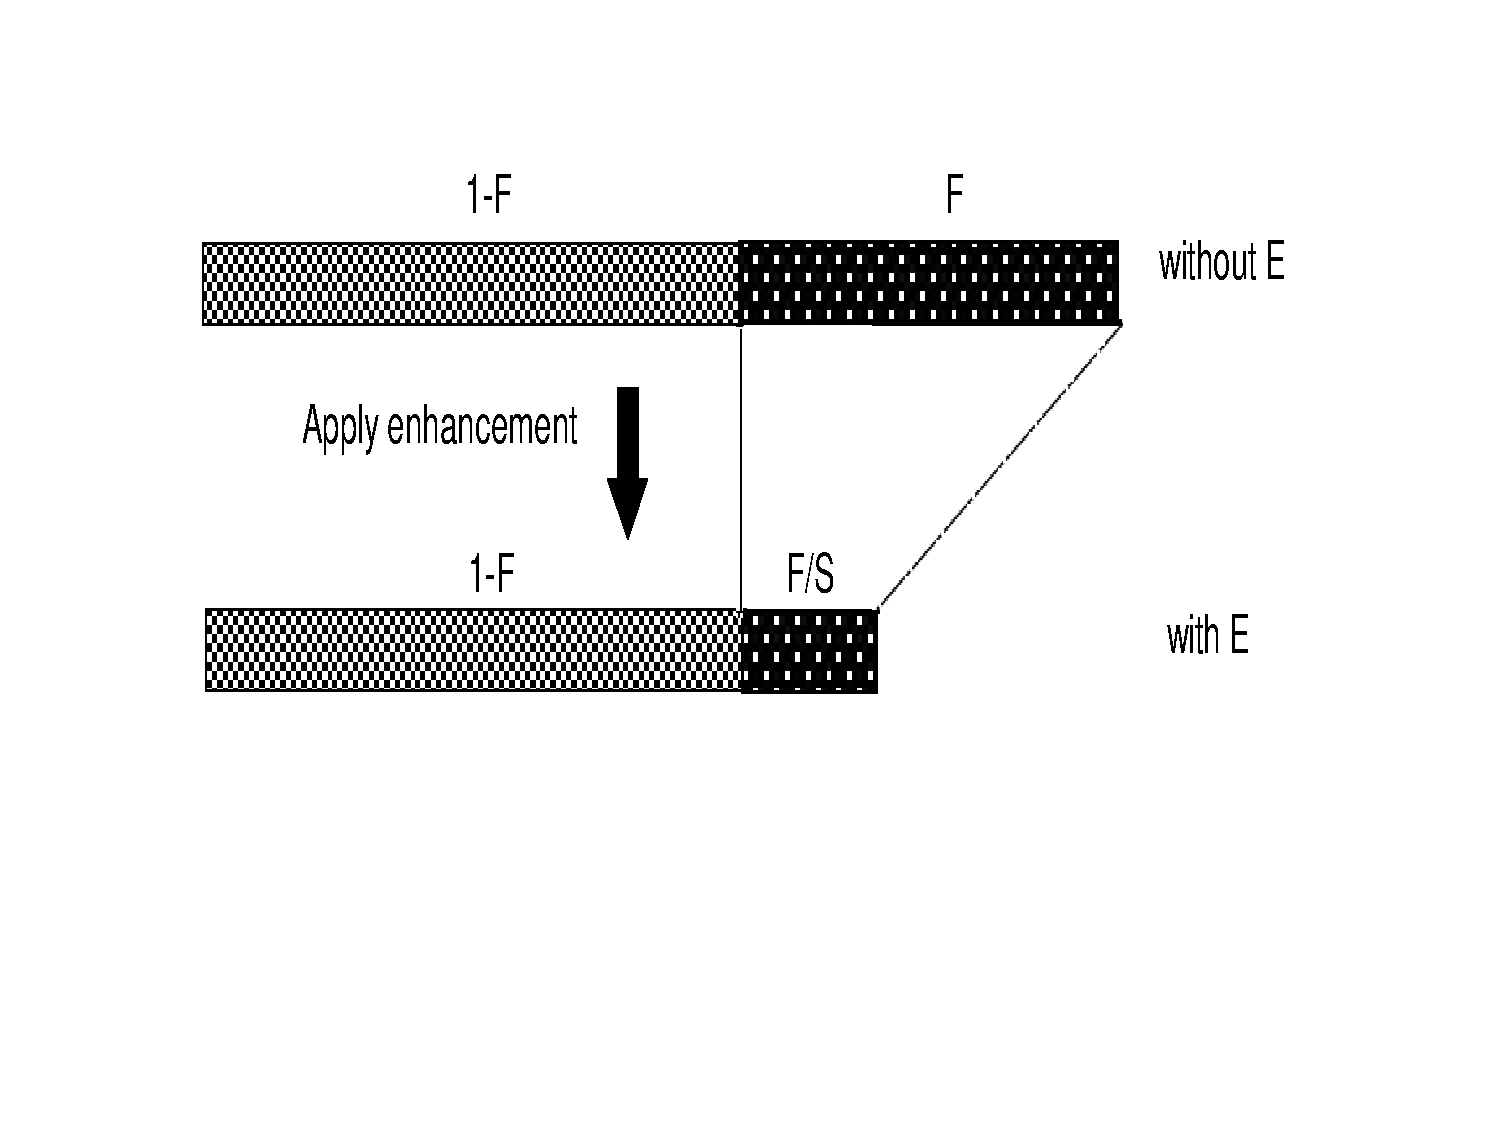
\includegraphics[width=50ex]{Figures/L2/Amdahl}\vspace{-15ex}
\caption{Enhancement $E$ accelerates a fraction $F$ of a program by a factor $S$.}
\label{fig:amdahl-assump}
\end{figure} 

Figure~\ref{fig:amdahl-assump} shows a scenario in which
an ``enhancement'' accelerates the computation of a fraction
$F$ of a program on a fixed dataset\footnote{
In general, a program running time is sensitive to the dataset,
so it does not makes sense to talk about speeding up a fraction
$F$ of a program in general---we need to fix the dataset.
} by a factor of $S$, while the other part of the program 
$1-F$ does not benefit from it.
(It is not important what the enhancement actually is,
or whether it is of software or hardware nature.)

In this scenario, the execution time of the enhanced program is:
\begin{center}
$T_{exe}(with E) = T_{exe}(without E)\times[(1-F) + \frac{F}{S}]$
\end{center}
Amdahl's Law correspond to (the interpretation of) three formulas:
one that computes the speedup of the enhanced program:
\begin{center}
$Speedup(E) = \frac{T_{exe}(without E)}{T_{exe}(with E)} = \frac{1}{(1-F)+\frac{F}{S}}$
\end{center}
and another two that compute an asymptotically-tight upper bound 
for the speedup when $S$ goes to infinity: 
\begin{center}
$Speedup(E) \leq \frac{1}{1-F}~~~~~$ and $~~~~~\lim_{S\to\infty}~Speedup(E) = \frac{1}{1-F}$
\end{center}

In essence, Amdahl's law shows that no matter how big the improvement is,
the overall application speedup is limited by the $1-F$ fraction that
does not benefit from the improvement.

\begin{figure}
\vspace{-4ex}
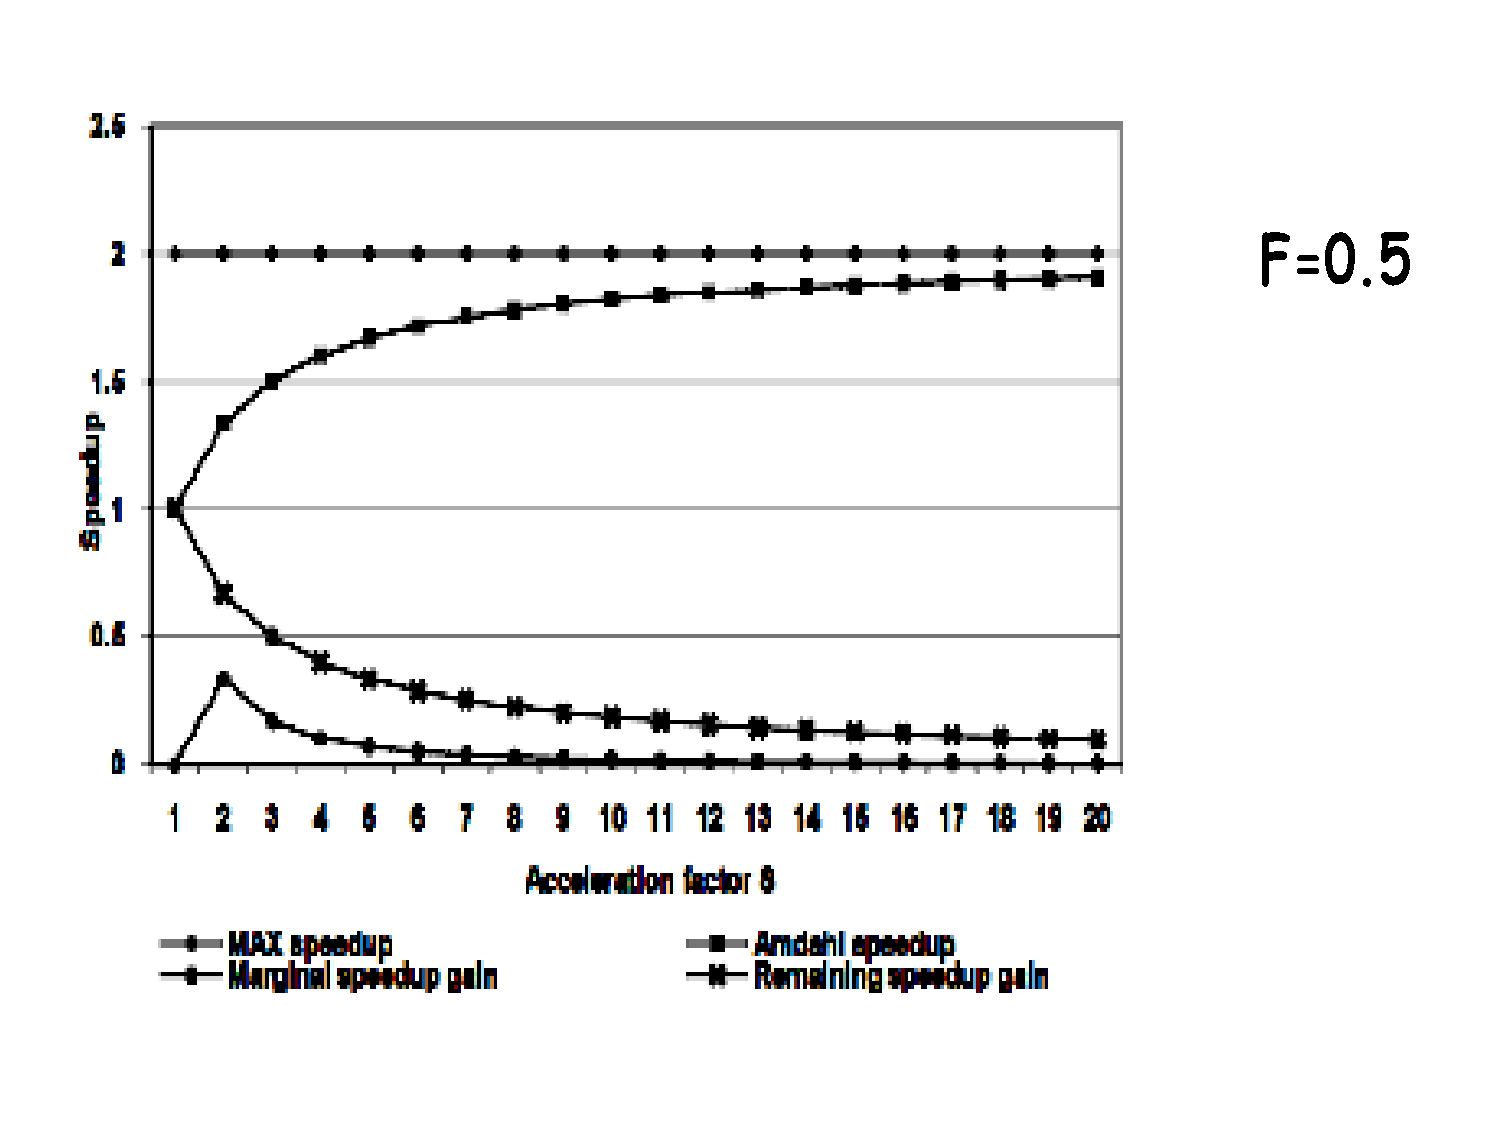
\includegraphics[width=90ex]{Figures/L2/AmdhalDimRet}\vspace{-7ex}
\caption{Interpretation of Amdahl's Law by Diminishing Returns. The $x$ and $y$ axis show the acceleration factor $S$ and the speedup, respectively. The lines appearing in the figure from top to bottom are: the maximal permitted speedup, the Amdahl's speedup, the remaining speedup gain, the marginal speedup gain (between two consecutive values of S).}
\label{fig:amdahl-interp}
\end{figure}

Figure~\ref{fig:amdahl-interp} shows a more detailed interpretation
of Amdahl's Law, specialized for the value $F = 0.5$, hence the maximal
speedup is $2\times$.   The figure demonstrates the law of diminishing
returns. It is reasonable to assume that every increment of $S$---shown
on the $x$ axis---requires the same amount of additional resources
(for enhancement). However, every increment of $S$ is less and less
rewarding globally. For example the step from $S=2$ to $S=3$ generates
an overall program speedup of $33\%$, while moving from $S=5$ to
$S=6$ generates a much smaller increase in speedup of only $6.67\%$. 
The moral of the story is to realize that some games cannot be 
won---the program speedup will never be higher than $2\times$---so
one should know when to stop, i.e., at the point when the next 
speedup gain will not justify the (extra) cost of the resources
necessary for implementing the next unit of enhancement.
In what hardware design is concerned, this would mean to implement
the ``common case\footnote{The common case is typically determined
by benchmarking.}'' in hardware (hence fast), and execute the rare
case in software (e.g., exceptions). 

\begin{figure}
\vspace{-4ex}
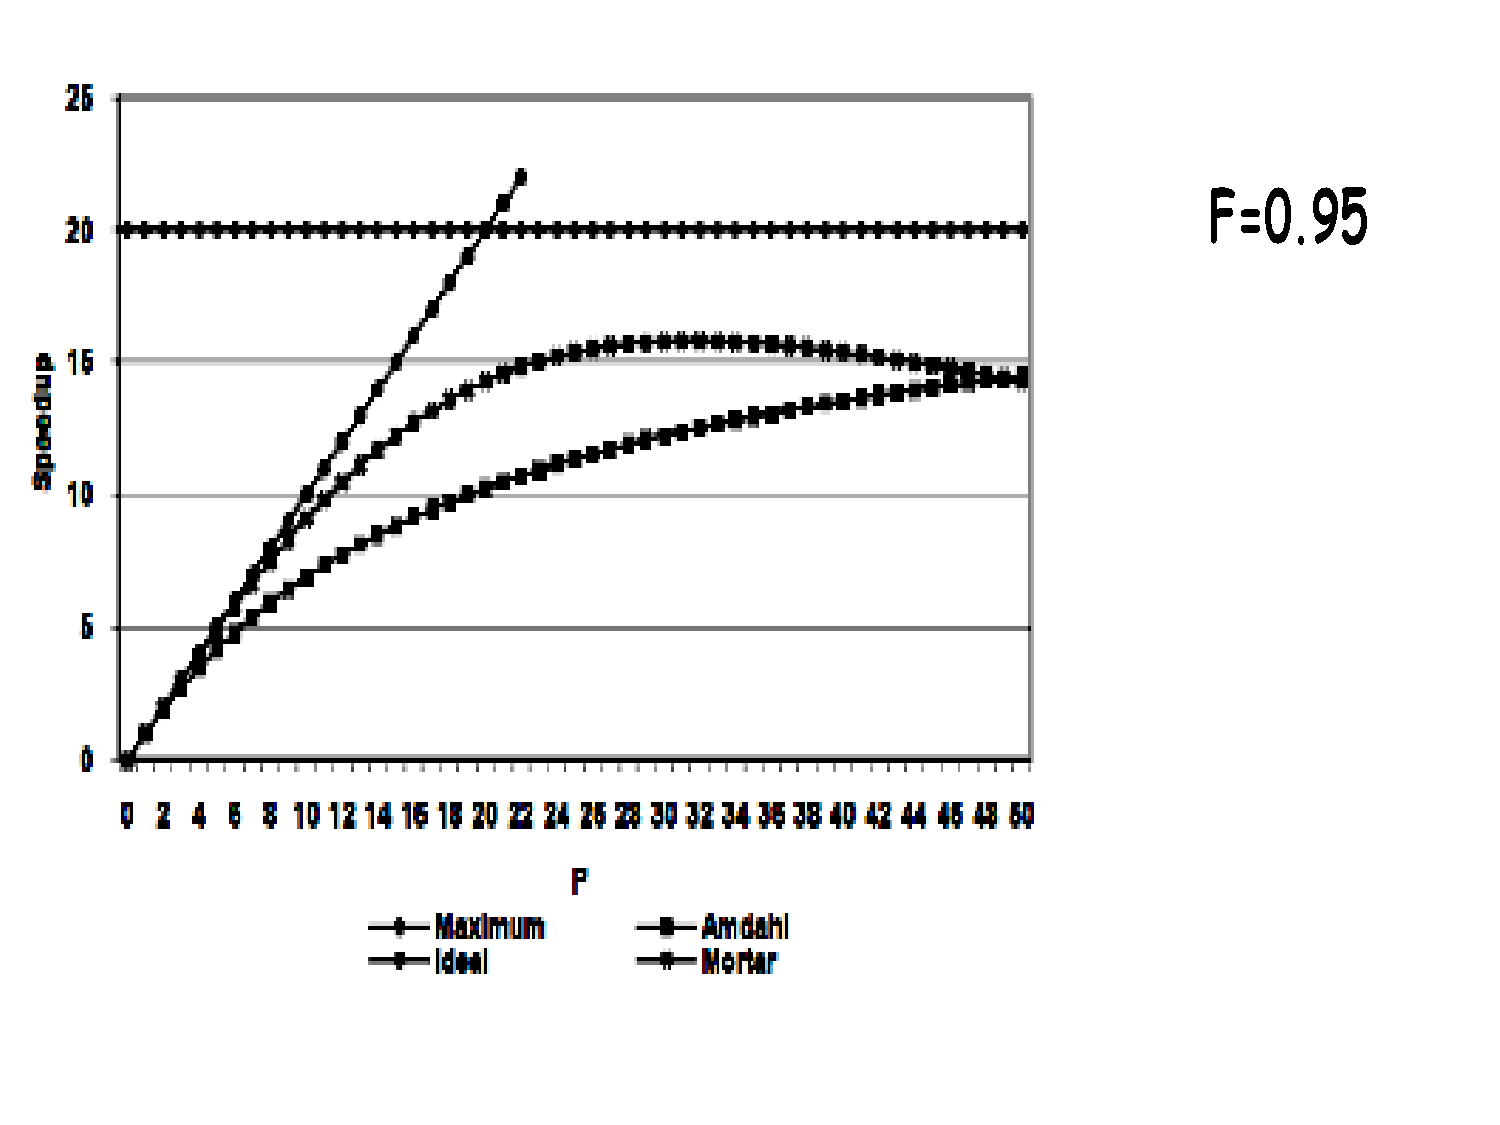
\includegraphics[width=90ex]{Figures/L2/AmdahlPar}\vspace{-7ex}
\caption{Demonstrating Amdahl's Law when the enhancement is 
parallel execution and $F=0.95$.\\ The mortar line shows a ``typical'' 
evolution of speedup in practice.}\vspace{-2ex}
\label{fig:amdahl-parallel}
\end{figure}

Figure~\ref{fig:amdahl-parallel} depicts the interpretation for
applying the Amdahl's law to the particular case of parallelism:
\begin{center}
$Speedup(P) = \frac{T_1}{T_P} = \frac{P}{F+P(1-F)}<\frac{1}{1-F}$
\end{center}
The specialization is straightforward: utilizing $P$ cores (rather 
than one) ideally results in a $P\times$ speedup. Actually, that 
is not quite true, since \emph{the occasional} super-linear speedup 
may be observed due to cache effects---the $P$ cores together have 
$P\times$ more cache than the uniprocessor, and applications 
with regular access patterns may benefit for the cache increase.
But typically, the speedup is sublinear even if $F=1$, because
for example threads might need to communicate and communication 
is expensive. One can observe that the Amdahl's law is unforgiving:
the figure uses $F=95$, which corresponds to $95\%$ of the runtime
being run in parallel; still the speedup is limited to $20\times$,
no matter how many cores you throw at it.

The moral of the parallel case is different than the one for the
general hardware improvement. We do not advocate to bound/restrict 
the number of cores just because some applications are inherently
sequential and will not benefit for extra parallelism. Quite the
contrary: after all, we have seen that scaling hardware parallelism
is the only conceivably way (nowadays) of keeping the Moore's Law
alive. 

What we advocate is to never leave sequential any part of 
the program that can possibly be parallelized. \emph{In other words, 
when developing parallel code, we must reason as if the hardware 
has an unlimited/infinity number of cores.}

Let me stress this further with an example that may catch your attention: 
assume the student has parallelized $99.9\%$ percent of the runtime of 
the application subject to the group project/exam. The student may feel 
entitled to receive the maximal grade, but the teacher might argue 
otherwise. The reason is that the GPUs that you are using in the PMPH 
course currently support $2880$ cores each.   Assume for the sake of 
the argument that each core run as fast as the CPU (they do not!). 
Applying Amdahl's law for $F=99.9\%$ results in a limiting
$1000\times$ speedup. This means that the student is only utilizing
about one third of the compute power provided by one GPU, and $35\%$
is a \emph{\bf failing grade}!\\
$\mbox{ }$\\

\subsubsection{Work-Depth Asymptotic Behavior of a Parallel Program}
\label{subsubsub:work-depth}
$\mbox{ }$\\

While there is a trend towards simplifying hardware, current hardware
remains way too complex for developing cost models based on them.
At least in what teaching is concerned, using a realistic hardware
model will put us in danger of ``missing the forest for the trees''. 
We will discuss parallel-program properties by reasoning about the
program execution on a very simple and idealized hardware model, 
named the parallel random access machine (PRAM). PRAM focuses on
(data) parallelism and completely ignores issues related to 
synchronization and communication. It assumes that:
\begin{itemize}
    \item there are $P$ processors that are connected to shared memory,

    \item each processor has an unique identifier/index $0 \leq i < P$,

    \item the execution happens in single-instruction multiple data (SIMD)
            fashion, which means that all cores execute in lock step---i.e.,
            a core cannot start the next instructions until all cores have
            completed executing the current instruction. Please note that
            in the case of an \lstinline{if-then-else}, the processors that
            did not take the \lstinline{then} branch must wait until all the
            other processors has finished executing the \lstinline{then} branch,
            before starting to execute the \lstinline{else} branch, and
            similar for the \lstinline{else} branch.

    \item each parallel instruction takes unit time (the same amount of time
            no matter whether it is a simple or complex arithmetic operation
            or a memory access).

    \item each processor has a flag that controls whether it is active in the
            execution of an instruction (for example in order to implement
            \lstinline{if-then-else}). If the processor is not active, then
            its {\tt noop} does not count towards the work complexity
            (but it counts towards the depth complexity, because it is
            part of a SIMD computational step).
\end{itemize}

We are ready to define the work-depth asymptotic behavior of a parallel
program on a PRAM machine. The work and depth computation assumes an
infinity number of processors ($P = \infty$).
\begin{itemize}
    \item \emph{\bf The work complexity} is the total number of operations
        performed to execute the program, i.e., the sum across all processors.
        We denote work by $W(n)$, where $n$ is related to the size of the
        dataset/workload.
    
    \item \emph{\bf The depth or step complexity}, denoted by $D(n)$ is 
        the number of sequential steps needed to execute the program.

    \item \emph{\bf A parallel implementation is work efficient} if its work
        complexity is asymptotically equal to that of the best sequential 
        implementation of the same algorithm.
\end{itemize} 

If we know (have computed) the work and depth of an implementation, then 
Brent's theorem specifies ``good'' complexity bounds for a PRAM that has
a finite number of $P$ cores, where by good we mean tight enough to be 
useful (for reasoning) in practice.

\begin{mytheo}[Brent's Theorem]\label{Brent-TH}
$\mbox{ }$\\
A parallel implementation that has depth $D(n)$ and work $W(n)$
can be simulated on a $P$-processor PRAM in time complexity $T$ 
such that:
\begin{center}
$\frac{W(n)}{P} \leq T \leq \frac{W(n)}{P} + D(n)$
\end{center}
\end{mytheo}

\subsubsection{Demonstrating Work-Depth Computation for Reduction}
\label{subsubsub:work-depth}
$\mbox{ }$\\

\begin{figure}
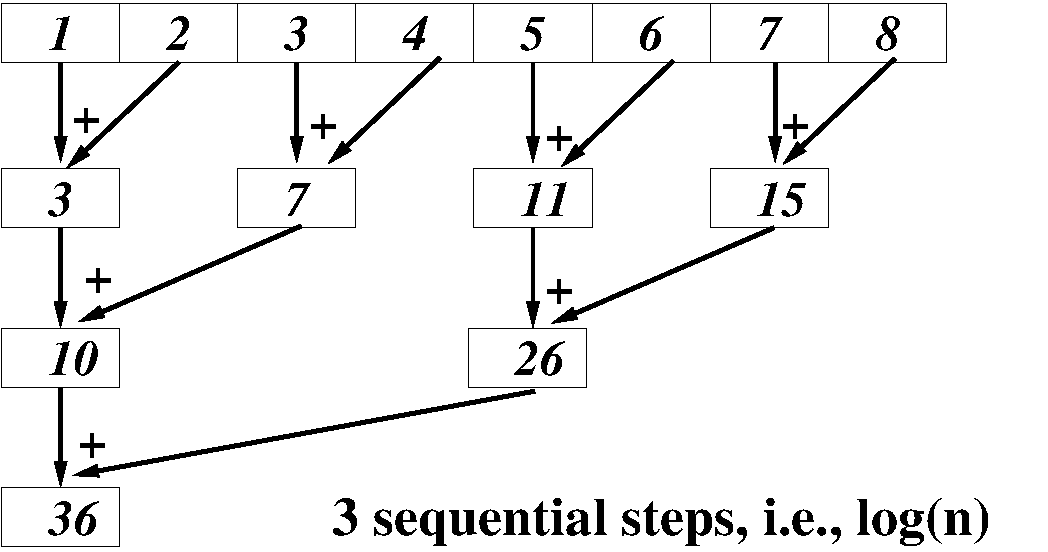
\includegraphics[width=40ex]{Figures/L1/ReduceEg.pdf}
\caption{Parallel execution of \lstinline{reduce} requires
        a sequence of \lstinline{log(n)} parallel operations
        ({\tt n} is the array length).}
\label{fig:red-tree-again}
\end{figure} 


The reduction tree for summing up (\lstinline{reduce (+) 0}) the elements 
of an array of $8$ elements is shown (again) in \cref{fig:red-tree-again}.
It is intuitively easy to generalize the work and depth for an array of
$n$ elements, which is summed up using $\frac{n}{2}$ processors:
\begin{itemize}
    \item the work is $W(n) = n$, hence parallel summation is work efficient
        because the best sequential algorithm still performs $O(n)$ steps;
    \item the depth is $D(n) = log(n)$, i.e., number of sequential steps;
    \item the optimized runtime on $P$ processors is actually 
            \emph{$O((n/P) + log(P))$.} This can be achieved by
            transforming the program according to \cref{Lemma-Map-Red}. 
            We recall that the ``Optimized-Map-Reduce Lemma'' says that
            a \lstinline{map-reduce} composition can be executed by:
        \begin{itemize}
            \item[(1)] chunking the input array into $P$ subarrays of roughly-equal 
            sizes,
            \item[(2)] then processing each subarray \emph{sequentially} on a 
            different processor, but \emph{in parallel} across subarrays,
            \item[(3)] then reducing the results of the $P$ subarrays
            in parallel by means of a reduction tree.
        \end{itemize}
            Step (1) and step (2) are fully parallel and take $O(n/P)$ time, 
            while step (3) requires 
            a reduction tree on $P$ elements, which takes $O(lg \ P)$ time (depth).
    \item one can now verify that Brent's lemma:\\
            \begin{center} $O(\frac{n}{P}) ~\leq ~O(\frac{n}{P} + log(P)) ~\leq~ O(\frac{n}{P} + log(n))$ \end{center}
          gives bounds which are good approximations (for the assumed $P \leq \frac{n}{2}$) 
            and allows us to reason on the essence rather than overthink the 
            impact of optimizations.
\end{itemize}

\begin{figure}
\begin{lstlisting}[mathescape=true]
Input:  array A of n=2$^k$ elems of type T
        $\oplus : T \rightarrow T \rightarrow T$ associative
Output: S = $\oplus_{j=1}^{n} a_j$

1.  forall i = 0 to n-1 do
2.    B[i] $\leftarrow$ A[i]
3.  endfor

4.  for h = 1 to k do
5.    forall i = 0 to n-1 by 2$^h$ do 
6.      B[i] $\leftarrow$ B[i] $\oplus$ B[i+2$^{h-1}$]
7.    endfor
8.  endfor
9.  S $\leftarrow$ B[0]  
\end{lstlisting}\vspace{-4ex}
\caption{Imperative, low-level pseudocode for parallel array summation.}
\label{fig-red-imp-pseudo}
\end{figure}

We have so far derived the work-depth complexity of array summations
in an intuitive way, by abstracting out the information depicted in 
a picture.   The question is: ``Can we also do this in a systematical
way for an arbitrary code?'' It turns out the answer is positive,
as demonstrated by the following analysis of the low-level (imperative)
pseudocode presented in \cref{fig-red-imp-pseudo}. The pseudocode
uses \lstinline{for} and \lstinline{forall} to denote a sequential and
a parallel loop, respectively. The analysis
proceeds bottom-up, by which we mean that we go in-order across
constructs at the same level and innermost-to-outermost in
nests:

\begin{itemize}
    \item The parallel loop between lines $1-3$ has 
            $D_{1-3}(n) = \Theta(1)$, and $W_{1-3}(n) = \Theta(n)$,
    \item The parallel loop between lines $5-7$ has
            $D_{5-7}(n) = \Theta(1)$, and $W_{5-7}(n,h) = \Theta(n/2^h)$,
    \item The sequential loop between lines $4-8$ executes $k$ 
            iterations ($n = 2^k$, hence $k = lg \ n$), each 
            consisting of the parallel loop $5-7$, 
            hence it has:
        \begin{itemize}
           \item depth $D_{4-8}(n) = k \times D_{5-7}(n) = \Theta(lg \ n)$, and
           \item work $W_{4-8}(n) = \sum_{h=1}^k W_{5-7}(n,h) = \Theta(\sum_{h=1}^k (\frac{n}{2^h}) ) = \Theta(2 n (1 - \frac{1}{2^{k+1}}) ) = \Theta(2 n (1 - \frac{1}{2 n}) ) = \Theta(n)$
        \end{itemize}
    \item The statement on line $9$ trivially has $D_{9}(n) = \Theta(1)$, $W_{9}(n) = \Theta(1)$,\bigskip
    \item Thus the depth and work for the entire program are
        \emph{$D(n) = \Theta(lg \ n), ~~\mbox{\tt and}~~ W(n) = \Theta(n)$}, respectively!
    \item By Brent's Theorem, it follows that the actual runtime is bounded by:
            $\frac{n}{P} \leq Runtime \leq \frac{n}{P} + lg \ n$
\end{itemize}

\subsubsection{Naive and Native Implementation of Reduction in Futhark}
\label{subsubsub:work-depth}
$\mbox{ }$\\

The previous section has shown that a reduction can be easily
implemented based on \lstinline{map}s and sequential loops.
It is natural to ask then, why does reduction need to be a
first-class citizen of a data-parallel language, when it can
be easily be provided as part of a library? 

We first provide an intuitive demonstration by implementing
reduction in the Futhark data-parallel language and comparing
the performance of our program with the natively supported
reduction. This also allows us to get acquainted with Futhark,
which will be used in PMPH exercises and so on.

\begin{figure}
\begin{lstlisting}[mathescape=true]
-- Reduction by hand in Futhark implemented in file: red-by-hand.fut
-- ==
-- compiled input {
--    [1.0f32, -2.0, -2.0, 0.0, 0.0, 0.0, 0.0, 0.0, 
--     3.0, 4.0, -6.0, 1.0, 2.0, -3.0, 7.0, 2.0]
-- }
-- output {
--    7.0f32
-- }
-- compiled input @ data/f32-arr-16777216.in
-- output { 3091.746094f32 }

-- For simplicity, assumes that n is 2^k
let main [n] (a : [n]f32) : f32 =
  let k = t32 <| f32.log2 <| r32 n
  let b = 
    loop b = a for h < k do
        let n' = n >> (h+1)
        in  map (\i -> unsafe (b[2*i]+b[2*i+1]) ) (iota n')
  in b[0]
\end{lstlisting}\vspace{-4ex}
\caption{Futhark Implementation for Summing Up an Array of Single-Precision Floats}
\label{fig:futhark-red}
\end{figure}

The Futhark implementation of the reduction pseudocode discussed
in the previous section is presented in \cref{fig:futhark-red}.
In the following, we will explain the code:
\begin{itemize}
    \item[(1)] In Futhark comments start with token {\tt --} and expand
            until the end of the line. However, an uninterrupted 
            sequence of comment lines that start a source file 
            (after the \lstinline{-- ==} comment) define 
            reference input-output datasets for automatic testing
            or benchmarking:

        \begin{itemize}
            \item The first dataset is directly specified:
            the input consists of an array of $16$ single-precision
            floats (\lstinline{f32}), using the common array literal 
            notation {\tt [a$_1$, $\ldots$, a$_n$]}, and the reference
            result is a single precision float {\tt 7.0f32}.

            \item The second dataset is held in a file 
            (\lstinline{-- compiled input @ data/f32-arr-16777216.in}),
            that stores an array of length $16777216$, but the result
            is given explicitly, albeit it can similarly be stored in
            a file (e.g., \lstinline{-- output @ data/f32-arr-16777216.out}).

            \item Assuming the name of the file is {\tt red-by-hand.fut},
                  compilation for GPU can be carried out with the command
            {\tt \$ futhark-opencl red-by-hand.fut} and compilation for
                  sequential C can be performed with  
            {\tt \$ futhark-c red-by-hand.fut}; both will result in an executable
            named {\tt red-by-hand}, which can be run on a dataset with the
            command:\\ 
            {\tt \$ red-by-hand -t /dev/stderr -r 10 < data/f32-arr-16777216.in}\\
            The {\tt -t} option records the program runtime (in microseconds)
            in the next-specified file; in our case this is displayed 
            in {\tt /dev/stderr}. The reported runtime {\bf does not include}:
            \begin{itemize} 
               \item the CPU-to-GPU transfer of the program input and the
            GPU-to-CPU transfer of the program result. 
               \item the OpenCL context creation and OpenCL kernel compilation.
            \end{itemize}
            Option {\tt -r 10} specifies that the runtime should be averaged
                across $10$ runs.
            If one wishes to inspect various profiling information, the
            program can be run with option {\tt -D}; this is especially
            useful when program compilation generates a number of kernels.

            \item Testing and benchmarking across the datasets specified in
            the source file itself can be carried out with the commands:\\
             {\tt \$ futhark-test  --compiler=futhark-opencl red-by-hand.fut}, or\\
             {\tt \$ futhark-bench --compiler=futhark-opencl red-by-hand.fut}

            \item random (uniformly-distributed) datasets can be created with
            the {\tt futhark-dataset} command (see help with the {\tt --help} option).
            An dataset consisting of an array of $16777216$ \lstinline{f32}
            elements can be produced and saved in file  {\tt data/f32-arr-16777216.in}
            by using the command:\\
            {\tt futhark-dataset -b --f32-bounds=-1.0:1.0 -g [16777216]f32 > data/f32-arr-16777216.in}
            
        \end{itemize}

    \item[(2)] Program execution starts with function {\tt main}.
          A function declaration starts with keyword \lstinline{let}
            followed by the function's name, which is optionally
            followed by declaring a set of variables that will be used
            to denote array sizes, for example \lstinline{[n][m][p]},
            followed by a sequence of typed formal arguments,
            and by the return type of the function.
        \begin{itemize}
          \item Our \lstinline{main} has one formal parameter, denoted
            {\tt a} which is an unidimensional array of single-precision 
            floats of length {\tt n}, i.e., (\lstinline{a: [n]f32}).   
          \item A three-dimensional array
            in which the sizes of the first and last dimension are {\tt n}
            and the size of the second dimension is {\tt m} would
            be written as \lstinline{[n][m][n]f32}, and {\tt m} would
            need to be declared similar to {\tt n}, i.e., {\tt [n][m]}.   
          \item In our case the result is a scalar: {\tt f32}.
                The programmer has to be a bit careful with the
                sizes of an array result type: a size which is declared
                in the optional part can be used in the array-result
                type if and only if it has been used in one of the
                formal array arguments. For example,
                \lstinline{let main [n] (a : [n]f32) : [n]f32 = ...}
                is legal and says that the input and result array should
                have the same length, but 
                \lstinline{let main [n] (m : f32) : [n]f32 = ...} is
                illegal because {\tt n} cannot be deduced from the inputs.
                In the latter case, what the user intends is probably 
                \lstinline{let main (n : i32) (m : i32) : [n]f32 = ...}.
        \end{itemize}
    \item[(3)] The program input and result  
            must be specified in tuple of arrays form (or structure of arrays AoS).
            (Note that this restriction only refers to the {\tt main} function   
            and entry points; all other code may use array-of-tuple form.)
            This is because the Futhark compiler automatically performs
            the AoS-to-SoA transformation in early compilation stages,
            but it obviously cannot also transform the program input.
            For example, it would be illegal to pass {\tt main}
            a formal argument \lstinline{b : [n](f32,f32)} or \lstinline{c : (f32, f32)}; 
            these should be split into two arguments each: 
            \lstinline{(b1: [n]f32) (b2: [n]f32)} or \lstinline{(c1: f32) (c2: f32)}.

    \item[(4)] The body of the {\tt main} is a \lstinline{let} expression.
        \begin{itemize}
              \item[1.] {\tt k} is bound to the value of {\tt log2 n}:\\
                \lstinline{let k = t32 <| f32 . log2 <| r32 n}\\
                where {\tt n} is assumed to be a power of two, and {\tt <|} pipes
                the right-hand side result to the left-hand side function (call): 
                \begin{itemize} 
                \item \lstinline{r32 n} transforms the $32$-bit integer \lstinline{n : i32}
                to a single precision float (\lstinline{f32}).
                \item \lstinline{f32.log2} calls the base-$2$ logarithm of the
                \lstinline{f32} module.
                \item \lstinline{t32} truncates the float argument to an \lstinline{i32}.
                \end{itemize}
              \item[2.] {\tt b} is defined to be the result of the \lstinline{loop}
                expression: \lstinline{loop b = a for h < k do body}, which is always
                executed sequentially: 
                \begin{itemize} 
                    \item {\tt b} is a variable bounded in the loop context, whose 
                value is variant across different iterations of the loop: it is initialized 
                upon loop entry with the value of {\tt a}, and the result of
                the loop {\tt body} will give the value of {\tt b} to be used by
                the next iteration of the loop.
                    \item the loop runs {\tt k} iterations (we recall that {\tt n = $2^k$})
                and {\tt h} takes values in {\tt 0, $\ldots$, k-1} in different iterations.
                Loops may also iterate across elements of an array using the more direct
                notation \lstinline{for x in xs}, such that {\tt x = xs[i]} in some iteration 
                {\tt i}.
                \end{itemize}
            \item[3.] The body of the loop consists of a \lstinline{let} expression:
            \begin{itemize}
                \item \lstinline{let n ' = n >> (h+1)} which binds {\tt n'} to the
                    value obtained by bit-shifting {\tt n} in the right direction with
                    {\tt h+1} bits, i.e., $n' = \frac{n}{2^{h+1}}$.
                \item and results in the application of \lstinline{map}
                    second-order array combinator (SOAC):\\
                    \lstinline{map (\i -> unsafe (b[2*i]+b[2*i+1]) ) (iota n')}
                    \begin{itemize}
                        \item the array input of the \lstinline{map} is \lstinline{iota n'}
                        which corresponds to the array {\tt [0,1,$\ldots$,n'-1]}.
                        \item the mapped anonymous (lambda) function is 
                        \lstinline{\i -> unsafe (b[2*i]+b[2*i+1]}.
                    \end{itemize}
                    Please note that the Futhark implementation differs from the
                    imperative pseudocode shown in \cref{fig-red-imp-pseudo} in that
                    each iteration of the Futhark loop computes an array result
                    of half the size of the input {\tt b}: iterations {\tt h=0},
                    {\tt h=1} and {\tt h=k-1} result in arrays of length 
                    $n' = \frac{n}{2^1}$, $n' = \frac{n}{2^2}$ and $n' = \frac{n}{2^k}=\frac{n}{n}=1$,
                    respectively.  That is the reason why all iterations use \lstinline{map}
                    with the same function \lstinline{\i -> unsafe (b[2*i]+b[2*i+1]}.
            \end{itemize}
            \item[4.] Finally the loop execution results in an array {\tt b} 
                containing one element, and the {\tt main} function returns
                the (first) element of {\tt b} (i.e., {\tt b[0]}).
        \end{itemize}

\end{itemize}

The second program, named {\tt red-native.fut} simply consists
of the code\\ 
\lstinline{let main [n] (a : [n]f32) : f32 = reduce (+) 0 a}
and we add the header used for testing/benchmarking.

Compiling and running the two programs on {\tt gpu04-diku-apl} 
shows that the native reduce is about a factor $8\times$ faster 
than our by-hand implementation ({\tt red-by-hand.fut}) based on
iterative \lstinline{map}s, on dataset {\tt data/f32-arr-16777216.in}:
 $321 \mbox{\tt vs} 2511$ microseconds.

The reason is that the code-generation of the native construct
benefits from an optimized code generation that executes \emph{one}
kernel\footnote{
The code generation of {\tt reduce} actually runs two kernels,
but the second one takes negligible time}
that performs about $n$ reads from global memory and much fewer 
writes to global memory, while using internally scratchpad (fast) 
GPU memory. 

In contrasts the discussed implementation ({\tt red-by-hand.fut})
executes a $24$-iteration loop ({\tt h = 0,$\ldots$,23}), in which 
each loop iteration calls a kernel corresponding to the \lstinline{map}
of size $n' = \frac{n}{2^{h+1}}$. The \lstinline{map} reads $2n'$ and 
writes $n'$ elements from/to global memory.
In total this implementation performs about $4 n$ reads and $2 n$ writes
from/to global memory.  The remaining difference can be explained 
by the overhead required to call an OpenCL kernel.

This is one of the reasons for which it makes sense to have second-order
array combinators (SOACs) such as \lstinline{reduce} and \lstinline{scan} as
first-class citizens in the data-parallel language. The other reason
corresponds to the algebraic properties of such operators: for example
the composition of a reduce and a map can be fused in a more
advanced construct~\cite{Futhark:redomap,Futhark:segredomap}, by a rule
similar to \cref{Lemma-Map-Red} which, similarly requires to read the 
input array once from global memory. 
Such high-level fusion rules would not be possible if we would implement
the {\tt reduce} in the library based on iterative applications of \lstinline{map};
it is even difficult to see how fusion could be applied in such a context.

\subsection{Other Parallel Operators, Examples of Nested-Parallel Applications}
\label{subsec:nest-par-app}

This section is organized as follows: 
\begin{itemize}
    \item \cref{subsubsub:var-par-ops} introduces
the type and semantics of several parallel operators commonly used in 
(functional) data-parallel languages. 
    \item \cref{subsubsub:scan-impl} presents
a possible, work-efficient implementation of the \lstinline{scan} 
(a.k.a. parallel-prefix sum) operator, which is a basic-block of
parallel programming, and shows how a segmented scan operator can
be easily written in terms of \lstinline{scan}. 

    \item \cref{subsubsub:filter-impl} shows a possible implementation of
\lstinline{filter} based on \lstinline{map} and \lstinline{scan}
and \lstinline{scatter} (parallel write) operators.

    \item The remaining (sub)sections demonstrate how 
        several applications can be constructed as puzzles from a nested
        composition of such operators:
        \begin{itemize}
        \item \cref{subsubsub:sparse-mat-vec-mult} briefly discusses
            the multiplication of a sparse matrix with a dense vector,
            and in particular introduces the notion of 
            \emph{\bf data flattening}.
        \item \cref{subsubsub:primes} presents three implementations for
            computing all prime numbers less then a certain input: 
            the first version provides the intuition, but does not have 
            the optimal depth; the second version fixes depth optimality,
            but this does not means it is necessarily best in practice;
            the last version is work inefficient but has a structure
            that makes it efficient for GPU hardware.
        \item Finally, \cref{subsubsub:quicksort} looks at the implementation
            of quicksort.
        \end{itemize}
\end{itemize}


\subsubsection{Types and Semantics of Various Parallel Operators}
\label{subsubsub:var-par-ops}
$\mbox{ }$\\

We start the discussion with \lstinline{zip} and \lstinline{unzip} operators:
\lstinline{zip} receives two arrays of the same length {\tt n} and produces
an array of tuples of length {\tt n} by pairing-up the elements at the same
index of the two arrays. \lstinline{unzip} is the inverse of \lstinline{zip}, 
i.e., \lstinline{unzip=zip}$^{-1}$:
\begin{lstlisting}[mathescape=true]
zip : $\Pi$n. [n]$\alpha_1$ $\to$ [n]$\alpha_2$ $\to$ [n]($\alpha_1,\alpha_2$)
zip [a$_1$,$\ldots$, a$_n$] [b$_1$,$\ldots$, b$_n$] = [(a$_1$,b$_1$),$\ldots$,(a$_n$,b$_n$)]
\end{lstlisting}\vspace{-1ex}

\begin{lstlisting}[mathescape=true]
unzip : $\Pi$n. [n]($\alpha_1,\alpha_2$) $\to$ ([n]$\alpha_1$, [n]$\alpha_2$)
unzip [(a$_1$,b$_1$),$\ldots$,(a$_n$,b$_n$)] = [a$_1$,$\ldots$, a$_n$] [b$_1$,$\ldots$, b$_n$]
\end{lstlisting}\vspace{-2ex}

Please note that our semantics differs from the one in Haskell, which would allow
two list of different length and would result in an array of tuples whose length
is the minimum of the input-array lengths.  In Futhark \lstinline{zip/unzip} are
syntactic sugar: they are supported in the source language, but are eliminated
(compiled away) in an early compiler stage that systematically rewrites the 
program to a tuple-of-arrays form.

We use the following array constructors:  
\begin{lstlisting}[mathescape=true]
iota : (n: i32) $\to$ [n]i32
iota n = [0,$\ldots$, n-1]
\end{lstlisting}\vspace{-1ex}

\begin{lstlisting}[mathescape=true]
replicate : (n: i32) $\to$ $\alpha$ $\to$ [n]$\alpha$
replicate n a = [a,$\ldots$, a]
\end{lstlisting}\vspace{-2ex}
\lstinline{iota n} creates an arrays of integral elements starting from {\tt 0} 
to {\tt n-1}, and \lstinline{replicate n a} creates an array of length {\tt n} 
filled with the same element {\tt a}. \lstinline{iota} can be used to create
the iteration space, for example in the case when the parallel operator needs
to access several elements of the input array in each iteration; we have seen
such an example in the case of the naive-reduce implementation:
\lstinline{map (\i -> unsafe (b[2*i]+b[2*i+1]) ) (iota n')}.
\lstinline{replicate} is typically used for initializing an array which will
be subject to a scan or to in-place updates.   

\begin{figure}
\begin{lstlisting}[mathescape=true]
map  : ($\alpha\to\beta$) $\to$ $\Pi$n. [n]$\alpha$ $\to$ [n]$\beta$
map  f [a$_1$, $\ldots$, a$_n$] = [f a$_1$, $\ldots$, f a$_n$]
map2 : ($\alpha1\to\alpha_2\to\beta$) $\to$ $\Pi$n. [n]$\alpha_1$ $\to$ [n]$\alpha_2$ $\to$ [n]$\beta$
map2 f [a$_1$, $\ldots$, a$_n$] [b$_1$, $\ldots$, b$_n$] = [f a$_1$ b$_1$, $\ldots$, f a$_n$ b$_2$]
map3 : $\ldots$

reduce : ($\alpha \to \alpha \to \alpha$) $\to$ $\alpha$ $\to$  $\Pi$n. [n]$\alpha$ $\to$ $\alpha$
reduce $\oplus$ 0$_{\oplus}$  [a$_1$, $\ldots$, a$_n$] = 0$_{\oplus}$ $\oplus$ a$_1$ $\oplus$ $\ldots$ $\oplus$ a$_n$

scan : ($\alpha \to \alpha \to \alpha$) $\to$ $\alpha$ $\to$ $\Pi$n. [n]$\alpha$ $\to$ [n]$\alpha$
scan $\oplus$ 0$_{\oplus}$ [a$_1$, $\ldots$, a$_n$] = [a$_1$, a$_1\oplus$a$_2$, $\ldots$, a$_1$ $\oplus$ $\ldots$ $\oplus$ a$_n$]

filter : ($\alpha$ $\to$ Bool) $\to$ $\Pi$n. [n]$\alpha$ $\to$ [m]$\alpha$   (where m $\leq$ n)
filter p [a$_1$, $\ldots$, a$_n$] = [a$_{k_1}$,$\ldots$, a$_{k_m}$]
  such that k$_1$ < k$_2$ < $\ldots$ < k$_m$, and denoting by $\overline{\mbox{\tt k}}$ = {k$_1$,$\ldots$, k$_m$},
  we have (p a$_j$ == true) $\forall$ j $\in$ $\overline{\mbox{\tt k}}$, and (p a$_j$ == false) $\forall$ j $\not\in$ $\overline{\mbox{\tt k}}$
\end{lstlisting}\vspace{-4ex}
\caption{Types and Semantics of \lstinline{map}s, \lstinline{reduce}, \lstinline{scan}, \lstinline{filter}.}
\label{fig:futhark-par-ops}
\end{figure}

Figure~\ref{fig:futhark-par-ops} shows the types and semantics of several second-order
array combinators (SOACs). We have already introduce \lstinline{map} and 
\lstinline{reduce} combinators. For ease of notation we will also introduce
\lstinline{map2} which receives as arguments a binary function {\tt f} and 
two input arrays of the same length, and produces an array by applying {\tt f}
to corresponding elements from the first and second arrays, respectively. 
Similar definitions are possible for {\tt map3} and so on.

\lstinline{scan} is commonly known as parallel-prefix sum, since it produces
an array of the same length as the input by starting with the first element,
then applying the operator between the first two elements, then applying the
operator between the first three elements, and so on, until the last element
corresponds to the result of reducing the array. Please note that, similar to
\lstinline{reduce}, \lstinline{scan}'s binary operator $\odot$ must be associative!
Please also note that the provided version of \lstinline{scan} is \emph{inclusive}
and it does not actually require a neutral element; an \emph{exclusive}
\lstinline{scan} requires a neutral element because it produces an array 
that starts with the neutral element and ends with the reduction of the 
first {\tt n-1} elements. The work and depth
of \lstinline{scan} is also similar to \lstinline{reduce}: $O(n)$ and $O(lg~n)$,
respectively.

Finally, \lstinline{filter} receives as argument a predicate {\tt p} 
(i.e., a function of type $\alpha\to${\tt{}Bool}) and an input array,
and it filters-out from the input array all the elements that do not
succeed under the predicate (i.e., indexes {\tt j} such that 
{\tt p a$_j$ = }\lstinline{false}). Please note that (i) the result
elements respect the relative order in which they appear in the input
array, and that (ii) the size of the result array is necessarily 
less than or equal to that of the input array. The work and depth
of \lstinline{filter} is similar to \lstinline{scan} 
($O(n)$ and $O(lg~n)$), because its implementation uses \lstinline{scan}. 

We conclude this subsection by introducing \lstinline{scatter},
a very important operator used for updating in parallel some of 
the indices of an arrays, where the updated indices do not necessarily
follow any regular pattern, i.e., think parallel random writes.
Its type is:\\
\lstinline{scatter}{\tt : $\Pi$ n. *[n]$\alpha~\to~\Pi$ m. [m]}\lstinline{i32}
{\tt$\to$ [m]$\alpha$ $\to$ *[n]$\alpha$}\\
which means that it receives as arguments a base array of length {\tt n},
and two arrays of length {\tt m} holding the to-be-updated
indices and corresponding values, respectively, and produces an array
of size {\tt n} by applying the updates. We make the following
important observations:
\begin{itemize}
    \item[(1)] The star {\tt *} in front of the type of the first input 
        array specifies that the array is going to be consumed---since
        the update is performed in place, it means that any following 
        reference to that array is \emph{illegal}! 
    \item[(2)] Furthermore, the first input (and the result) array cannot 
        alias the other two 
        array arguments. This would not be necessary on a PRAM machine
        with an infinity number of cores that execute in SIMD fashion,
        but such hardware does not exist in practice.
    \item[(3)] The depth of \lstinline{scatter} is $O(1)$, and its work is 
        $O(m)$---meaning, it does not depend on {\tt n}, the size of 
        the to-be-updated array.
\end{itemize}
For programming convenience (e.g., padding), we enrich the semantics
of \lstinline{scatter} by requiring that the indices that are 
outside the bounds of the input array are simply ignored (are not
updated). As such {\tt n} and {\tt m} are in no relation with
each other: it can be that {\tt n<m} or {\tt n==m} or {\tt n>m}. 

We conclude with an example that hopefully clarifies how 
\lstinline{scatter} works:
\begin{lstlisting}[mathescape=true]
X (input  array) = [a$_0$, a$_1$, a$_2$, a$_3$, a$_4$, a$_5$]
I (index vector) = [2, 4, -1, 1]
D (data  vector) = [b$_0$, b$_1$, b$_2$, b$_3$]
scatter X I D    = [a$_0$, b$_3$, b$_0$, a$_3$, b$_1$, a$_5$]
\end{lstlisting}\vspace{-2ex}


\subsubsection{Implementation of Scan and Segmented Scan}
\label{subsubsub:scan-impl}
$\mbox{ }$\\

We start by emphasizing again that, similar to \lstinline{reduce},
\lstinline{scan} requires an \emph{\bf associative} binary operator,
and the exclusive scan requires the neutral element of the monoid 
induced by that operator.

\begin{figure}
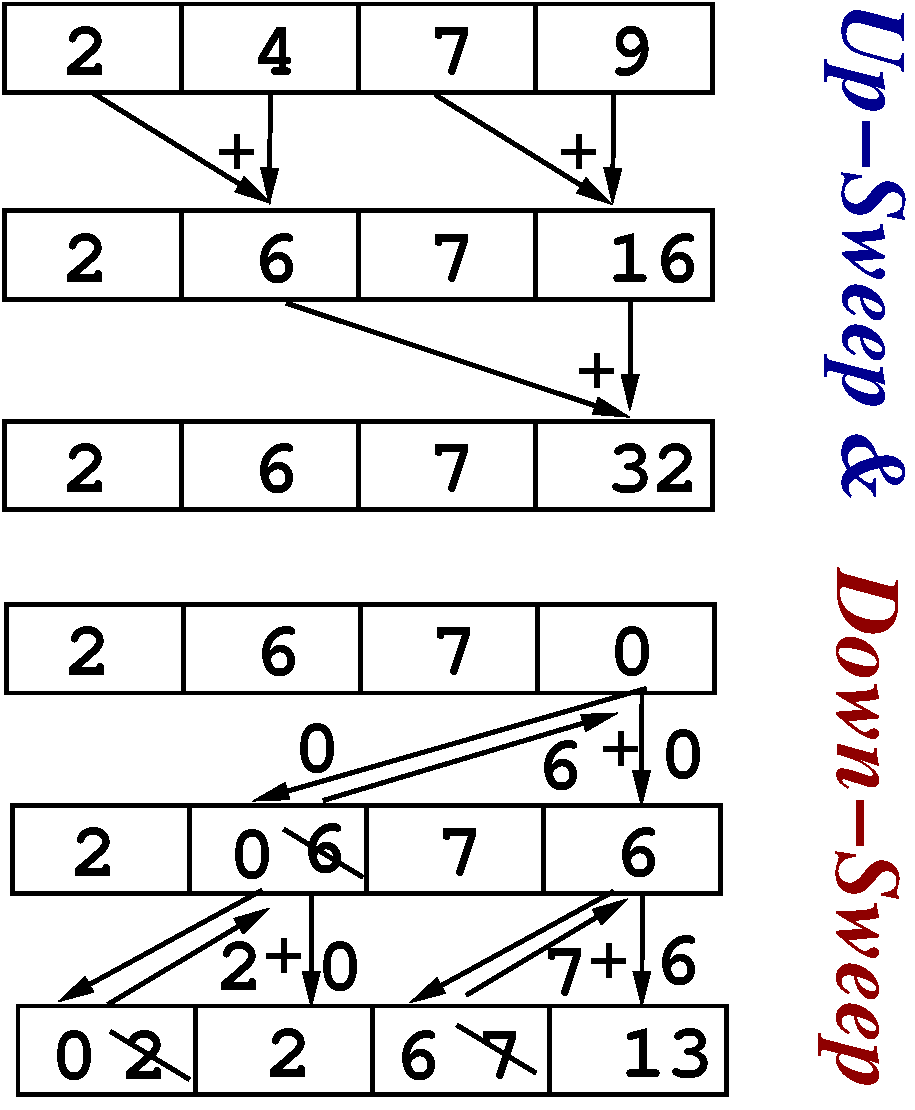
\includegraphics[height=33ex]{Figures/L2/ScanEg.pdf} 
\caption{Parallel execution of \lstinline{scan} for a $4$-element array.}
\label{fig:scan-eg}
\end{figure} 

The intuition behind the implementation of exclusive scan is depicted
in \cref{fig:scan-eg} for an array of four elements. Note that its
semantics differs from that of Futhark's (inclusive) scan: assuming an
{\tt n}-element input array, an exclusive scan results in the neutral 
element in the first position of the result array, and the ``sum'' of 
the first {\tt n-1} elements in position {\tt n-1}. 
The implementation is organized in two parallel steps:
\begin{itemize}
    \item[(1)] The first step is called ``Up-Sweep'' and is similar 
                with a reduction, except that the accumulation of
                all elements is computed in the last element of 
                the array, rather than the first.
    \item After the up-sweep pass, value $0$ is placed in the position
                of the last element. 
    \item[(2)] The second step is called ``Down-Sweep'', and it 
                propagates updates to the array's elements in the 
                reverse order of the up-sweep pass (i.e., reverse the arrows 
                and the traversal of the up sweep). Each propagation
                requires two substeps:
             \begin{itemize}
                \item[2.1.] the left child sends its value to its parent 
                    and updates its value to that of the parent. 
                \item[2.2.] the right-child value is obtained by applying
                            the binary operator of the scan to the left-child 
                            value and to the (old) value of parent.
                Please notice that the right child is in fact the
                            parent---an in-place algorithm.
             \end{itemize}
\end{itemize}


\begin{figure}
\begin{lstlisting}[mathescape=true]
Input:  array A of n=$2^k$ elements of type $\alpha$
        $\oplus$ : $\alpha\to\alpha\to\alpha$ associative
Output: B = [0, a$_1$, a$_1$$\oplus$a$_2$,$\ldots$,$\oplus_{j=1}^{n-1}$ a$_j$]

1.  forall i = 0 : n-1 do
2.    B[i] $\leftarrow$ A[i]
3.  endfor

4.  for d = 0 to k-1 do -- up-sweep pass
5.    forall i = 0 to n-1 by 2$^{d+1}$ do 
6.      B[i+2$^{d+1}$-1] $\leftarrow$ B[i+2$^{d}$-1] $\oplus$ B[i+2$^{d+1}$-1]
7.    endfor
8.  endfor
9.  B[n-1] = 0
10. for d = k-1 downto 0 do -- down-sweep pass
11.   forall i = 0 to n-1 by 2$^{d+1}$ do 
12.     tmp $\leftarrow$ B[i+2$^d$-1]
13.     B[i+2$^d$-1] $\leftarrow$ B[i+2$^{d+1}$-1]
14.     B[i+2$^{d+1}$-1] $\leftarrow$ tmp $\oplus$ B[i+2$^{d+1}$-1]
15.   endfor
16. endfor
\end{lstlisting}\vspace{-4ex}
\caption{Imperative Pseudcode for implementing exclusive scan}
\label{fig:imperative-scan-exc}
\end{figure}

The imperative pseudocode that implements the exclusive scan operator
is shown in \cref{fig:imperative-scan-exc}. A reasoning similar to the
one we applied to \lstinline{reduce} can compute that the depth and work
of the presented implementation is $D(n) = \Theta(lg \ n)$ and 
$W(n) = \Theta(n)$, respectively. In fact the only difference in
comparison to the imperative pseudocode of reduce is that scan
requires an extra (down-sweep pass), but this does not matter
complexity-wise because it has the same work and depth as the
up-sweep pass (similar to the one used for reduction), and
a $2\times$ factor leaves unchanged the asymptotic behavior.

\begin{figure}
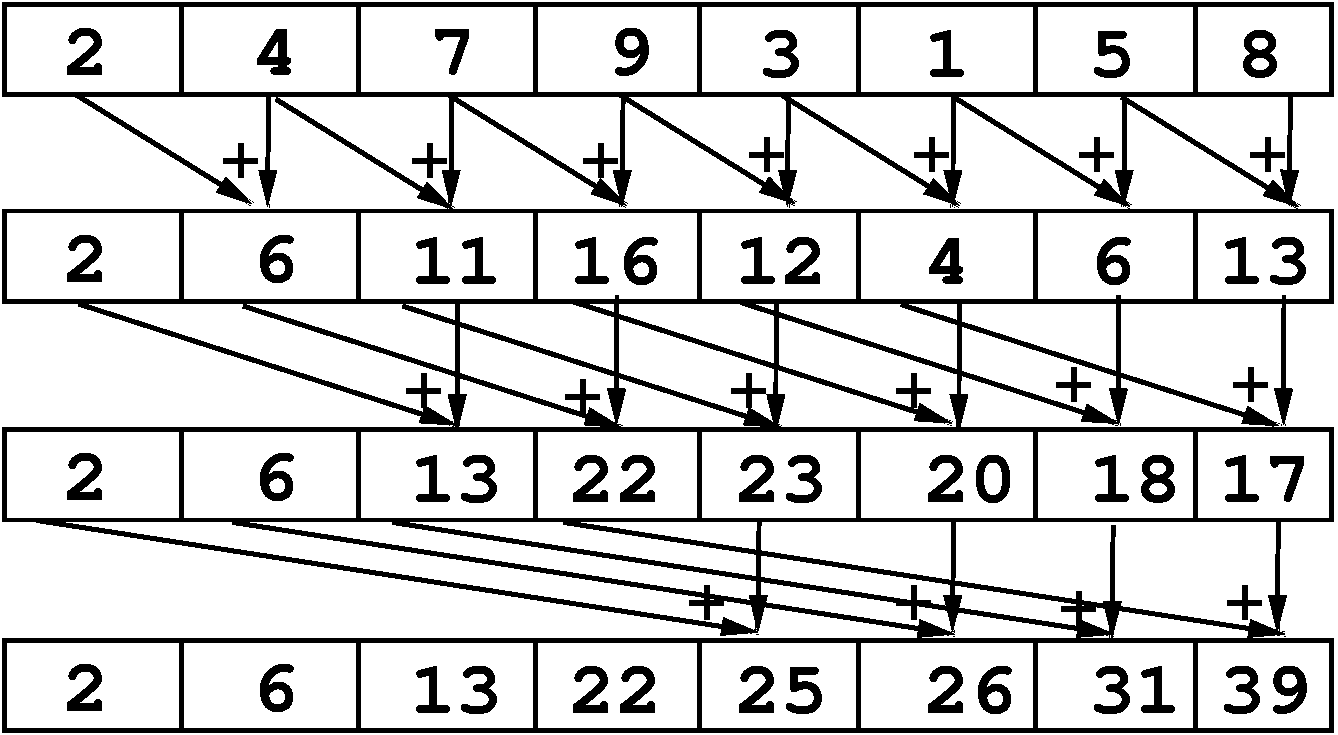
\includegraphics[height=30ex]{Figures/L2/SgmScanEg.pdf} 
\caption{Inclusive \lstinline{scan} used inside a warp for CUDA implementation.}
\label{fig:scan-eg-warp}
\end{figure} 

\begin{figure}
\begin{lstlisting}[mathescape=true]
Input:  array A of n=$2^k$ elements of type $\alpha$
        $\oplus$ : $\alpha\to\alpha\to\alpha$ associative
Output: B = [a$_1$, a$_1$$\oplus$a$_2$,$\ldots$,$\oplus_{j=0}^{n-1}$ a$_j$]
1.  forall i = 0 : n-1 do
2.    B[i] $\leftarrow$ A[i]
3.  endfor
4.  for d = 0 to k-1 do
5.    h = 2$^d$
6.    forall i = h to n-1 do 
7.      B[i] $\leftarrow$ B[i-h] $\oplus$ B[i]
8.    endfor
9.  endfor
\end{lstlisting}\vspace{-4ex}
\caption{Imperative Pseudcode for warp-level inclusive scan in CUDA; $n=32$}
\label{fig:warp-scan-inc}
\end{figure}

The pattern of a work-inefficient algorithm for inclusive scan is shown
in \cref{fig:scan-eg-warp}, and the pseudocode is presented in 
\cref{fig:warp-scan-inc}. This is the typical CUDA implementation
for a warp of threads---a warp is the unit of parallel execution
in CUDA and consists of $32$ consecutive threads.  Note that
the depth of the implementation is optimal: $D(n) = \Theta(lg \ n)$,
but the work is not:  $W(n) = \Theta(n~lg~n)$. However, on CUDA
platforms, any warp of threads executes in lock-step (in SIMD fashion), 
and de-selecting threads from execution (within one warp) brings no 
benefits. In fact this implementation is a factor of $2\times$ faster
than the one based on the up- and down-sweep, because it performs
only one sweep---its depth is $lg~n$ instead of $2~lg~n$. 

The remaining of this (sub)section discusses the \textbf{\em segmented scan} 
operator. A segmented scan semantically operates on an array of arrays---think 
a matrix in which the rows do not necessarily have the same length---and it
results in an array of arrays of similar shape as the input, in which each
of the resulted subarrays are obtained by scanning the corresponding input
subarray with the given associative binary operator (and neutral element).
Thus the semantics of a segmented scan is a map over the input array, in 
which the mapped function performs a scan on each subarray. The example
below demonstrates the semantics of an inclusive segmented scan:
\begin{lstlisting}[mathescape=true]
sgmScan (+) 0 [[1,3,5], [7,8], [9,11,14,15]] $\equiv$
[scan (+) 0 [1,3,5], scan (+) 0 [7,8], scan (+) 0 [9,11,14,15]] $\equiv$
[[1,4,9], [7,15], [9,20,34,49]]
\end{lstlisting}\vspace{-2ex}

The example above specifies the semantics but does not give insight into
what a data-parallel implementation should be. The major obstacle is that
the array of arrays is typically represented as an array of pointers,
each pointing to the corresponding subarray.
However this representation is not suitable for parallel execution: we 
need a flat data-structure! As such, we represent the array of arrays 
by a flat array of \emph{values}---whose length {\tt n} is the total
number of elements, i.e., the sum of the lengths of the subarrays---together 
with a \emph{flag} array, which has {\tt 1} (or \lstinline{true}) in the 
first position that starts a subarray, and {\tt 0} (or \lstinline{false}) 
in the remaining positions. One may also add to the representation a
shape array, which has number-of-subarrays integral elements, each
containing the lengths of its corresponding subarray. We present an 
example below that demonstrates the data-parallel representation 
(shape + flag + value flat arrays):
\begin{lstlisting}[mathescape=true]
nestedArray = [[1, 3, 5], [7, 8], [9, 11, 14, 15]]
   $\downarrow$            $\downarrow$          $\downarrow$        $\downarrow$
shapeArray  = [ 3,         2,      4             ]
flagArray   = [ 1, 0, 0,   1, 0,   1, 0,   0, 0  ]
valueArray  = [ 1, 3, 5,   7, 8,   9, 11, 14, 15 ]
\end{lstlisting}\vspace{-2ex}

It follows that the segmented scan has almost the same type as scan,
the only difference being that it receives one extra argument: the flag
array, which is represented as an array of booleans (or integers):
\begin{lstlisting}[mathescape=true]
sgmScan : ($\alpha\to\alpha\to\alpha$) $\to$ $\alpha$ $\to$ $\Pi$ n. [n]bool $\to$ [n]$\alpha$ $\to$ [n]$\alpha$
\end{lstlisting}\vspace{-2ex}
%We also note that the shape array is not necessary for the implementation
%of segmented scan.

\begin{figure}
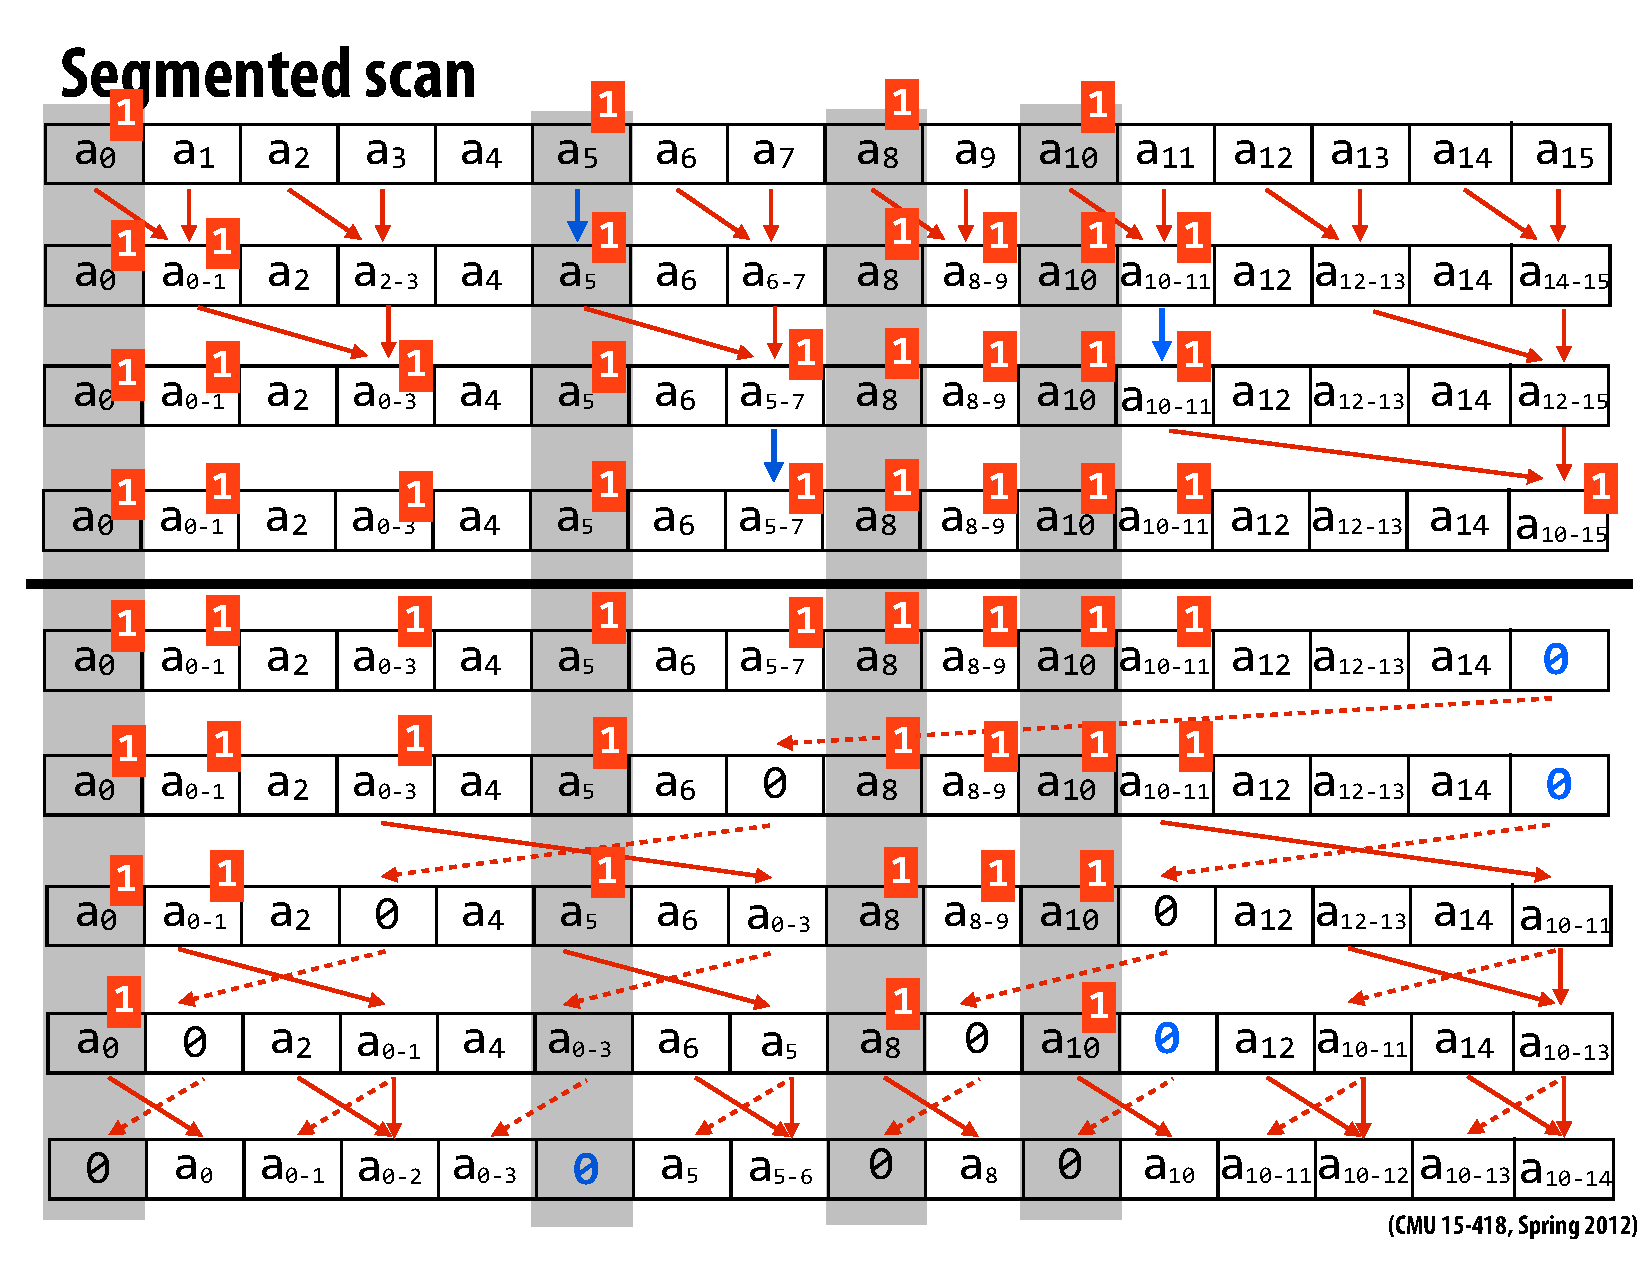
\includegraphics[height=55ex]{Figures/L2/Sgm-Excl-Scan-Eg.pdf} 
\caption{Parallel execution of exclusive segmented scan. Figure courtesy of CMU 15-418, Spring 2012}
\label{fig:sgm-scan-eg}
\end{figure} 

\begin{figure}
\begin{lstlisting}[mathescape=true]
Input:  flag array F of n=2$^k$ of ints/bools
        data array A of n=2$^k$ elements of type $\alpha$
        $\oplus$ : $\alpha\to\alpha\to\alpha$ associative
Output: B = segmented scan of 2-dimensional (irregular) array A
1.  forall i = 0 to n-1 do B[i] $\leftarrow$ A[i] endfor
2.  for d = 0 to k-1 do -- up-sweep pass
3.    forall i = 0 to n-1 by 2$^{d+1}$ do 
4.      if F[i+2$^{d+1}$-1] == 0 then 
5.          B[i+2$^{d+1}$-1] $\leftarrow$ B[i+2$^{d}$-1] $\oplus$ B[i+2$^{d+1}$-1]
6.      endif
7.      F[i+2$^{d+1}$-1] $\leftarrow$ F[i+2$^{d}$-1] .|. F[i+2$^{d+1}$-1] -- .|. is bitwise-or
8.  endfor endfor
9.  B[n-1] $\leftarrow$ 0
10. for d = k-1 downto 0 do -- down-sweep pass
11.   forall i = 0 to n-1 by 2$^{d+1}$ do 
12.     tmp $\leftarrow$ B[i+2$^{d}$-1]
13.     if F_original[i+2$^{d}$] $\neq$ 0 then
14.          B[i+2$^{d+1}$-1] $\leftarrow$ 0
15.     else if F[i+2$^{d}$-1] $\neq$ 0 then
16.          B[i+2$^{d+1}$-1] $\leftarrow$ tmp
17.     else B[i+2$^{d+1}$-1] $\leftarrow$ tmp $\oplus$ B[i+2$^{d+1}$-1]
18.     endif
19.     F[i+2$^{d+1}$-1] $\leftarrow$ 0
20. endfor endfor
\end{lstlisting}\vspace{-4ex}
\caption{Imperative Pseudcode for implementing exclusive segmented scan}
\label{fig:imperative-sgm-scan-exc}
\end{figure}



For completeness, \cref{fig:sgm-scan-eg} shows a graphical representation
of the execution pattern of exclusive segmented scan, and 
\cref{fig:imperative-sgm-scan-exc} shows the imperative pseudocode for
exclusive segmented scan. While there are more branches, it is relatively
straightforward to see that the depth and work asymptotics of segmented
scan remains the same as the one of scan: $D(n) ~=~ \Theta(lg~n)$ and
$W(n) ~=~ \Theta(n)$.   Understanding the execution pattern and pseudocode
is difficult: the teacher advices to {\em not} attempt it because
it does not really provide essential new insight. 

Instead, we make the \textbf{\em essential observation} that a segmented 
scan can be straightforwardly implemented in terms of a scan, which basically 
means that if an efficient implementation of scan is given, then we can 
directly derive an efficient implementation of segmented scan, and moreover,
that segmented scan has the same work and depth complexity as scan.


The code below shows the Futhark implementation of the inclusive segmented scan:
\begin{lstlisting}[mathescape=true]
let segmented_scan [n] 't (op: t -> t -> t) (ne: t)
                          (flags: [n]bool) (arr: [n]t): [n]t =
  let (_, res) = unzip <|
    scan (\(x_flag,x) (y_flag,y) -> -- extended binop is denoted $\odot$
             let fl = x_flag || y_flag
             let vl = if y_flag then y else x `op` y
             in  (fl, vl)
         ) (false, ne) (zip flags arr)
  in  res
\end{lstlisting}\vspace{-2ex}
The implementation consists of a \lstinline{scan} whose
input array is obtained by zipping the flag and value arrays, and
whose binary associative operator combines two flag-value tuples:
\begin{itemize}
    \item {\tt (x\_flag,x)} is the accumulator and {\tt (y\_flag,y)} 
        corresponds to the flag and value of the current element of 
        the input array;
    \item  the segmented-scan operator computes the resulting value
        by checking whether the current element corresponds to the start
        of a segment (i.e., tests whether {\tt y\_flag} is true).
        \begin{itemize}
            \item if this is the start of a segment, then
                the resulting value is the current element
                value ({\tt y}), as dictated by the semantics
                of inclusive segmented scan;
            \item otherwise we need to accumulate the current
                value: \lstinline{x `op` y}
        \end{itemize}
    \item the segmented-scan operator computes the resulting flag
        by taking the logical or of the two argument flags. This is
        necessary in order to propagate the start-of-a-segment flag,
        because parallel execution may proceed in a different order
        than the sequential execution. 
    \item We leave as an exercise to verify that the scan's operator is 
        associative, i.e.,\\
        {\tt ((x\_flag,x) $\odot$ (y\_flag,y)) $\odot$ (z\_flag,z)} equals\\
        {\tt (x\_flag,x) $\odot$ ((y\_flag,y) $\odot$ (z\_flag,z))},
        and the check that the neutral element
        of the monoid induced by $\odot$ is indeed \lstinline{(false, ne)}.
\end{itemize}

\textbf{\em An important observation} is that segmented scan can be easily 
adapted to work with an integral array of flags, in which a flag different 
than $0$ denotes the start of a new segment. The necessary modifications are:
\begin{itemize}
    \item {\tt fl = x\_flag || y\_flag} is rewritten as {\tt fl = x\_flag | y\_flag},
            where {\tt |} denotes the bitwise-or operator, and
    \item the branch condition {\tt if y\_flag} is rewritten as
            {\tt if y\_flag != 0}.
\end{itemize}
Maintaining the flags as an array of boolean reduces memory footprint and
saves bandwidth, but some of the flattening rules can be optimized if we
use the integral representation.

\subsubsection{Implementation of Partition (Filter)}
\label{subsubsub:filter-impl}
$\mbox{ }$\\

We have already presented the type and semantics of \lstinline{filter}.
The question is: ``can filter be implemented in terms of \lstinline{map},
\lstinline{scan}, and \lstinline{scatter}?''
The answer is positive! 

In the following we will derive the implementation of a slightly more complicated 
construct than filter, named \lstinline{partition}, which has type:
\begin{lstlisting}[mathescape=true]
partition2 : ($\alpha~\to~$bool) $\to$ $\Pi$ n. [n]$\alpha$ $\to$ ([n]$\alpha$,i32) 
\end{lstlisting}\vspace{-2ex}
Partition is similar to \lstinline{filter}, in that it receives
as arguments a predicate and an input array, but it returns
an array of the same length as the input array and an integer.
The array result contains the same elements as the input array,
but in a different order: 
\begin{itemize}
    \item the elements that succeed under the predicate
            come before the ones that fail the predicate,
    \item the relative order of the elements in the two
            subarrays is the same as in the original array.
\end{itemize}
The scalar (integral) result is the number of elements that succeed 
under the predicate. 

\begin{figure}
\begin{lstlisting}[mathescape=true]
let partition2 [n] 't                    -- Assume t = i32, n = 6,
           (p : (t -> bool))             -- p (x:i32)= 0 == (x%2),
           (arr : [n]t) : ([n]t, i32) =  -- arr = [5,4,2,3,7,8]
  let cs  = map p arr                    -- cs  = [F,T,T,F,F,T]
  let tfs = map (\f -> if f then 1       -- tfs = [0,1,1,0,0,1]
                            else 0) cs
  let isT = scan (+) 0 tfs               -- isT = [0,1,2,2,2,3]
  let i   = isT[n-1]                     -- i   = 3

  let ffs = map (\f->if f then 0 
                          else 1) cs     -- ffs = [1,0,0,1,1,0]
  let isF = map (+i) <| scan (+) 0 ffs   -- isF = [4,4,4,5,6,6]
  let inds= map3 (\c iT iF ->            -- inds= [3,0,1,4,5,2]
                    if c then iT-1 
                         else iF-1
                 ) cs isT isF
  let r = scatter (scratch n t) inds arr -- r = [4,2,8,5,3,7]            
  in  (r, i) 
\end{lstlisting}\vspace{-4ex}
\caption{Implementation of a two-way partition in Futhark.}
\label{fig:futhark-partition2}
\end{figure}

The Futhark implementation is shown in \cref{fig:futhark-partition2};
the last {\tt let} instruction uses the {\tt scratch} operator
that creates an uninitialized array of size {\tt n} and element
type {\tt t}; please note that the result of {\tt partition2} is 
still deterministic because it is guaranteed that all elements
are going to be written by \lstinline{scatter}. 
%
The right hand  side of \cref{fig:futhark-partition2} demonstrates
the code on an example. The implementation proceeds as follows:
\begin{itemize}
    \item First, the predicate is mapped on the input array,
            and the result is turned into ones (for \lstinline{true})
            or zeros (for \lstinline{false}), which are stored in
            array {\tt tfs}.
    \item An inclusive scan with addition is performed on {\tt tfs}
            resulting in array {\tt isT}. Please observe that 
            array {\tt isT} now holds the value of the indices at 
            which the elements that succeed under the predicate
            should appear in the result array (plus one). Also
            the last element of {\tt isT}, saved under variable 
            {\tt i} is the number of elements that succeed under 
            the predicate.
    \item Array {\tt isF} is computed in a similar fashion and
            holds the value of the indices at which the elements 
            that fail under the predicate
            should appear in the result array (plus one).
    \item The two pieces of information are combined together
            in array {\tt inds} from arrays {\tt isT} and {\tt isF}
            (and {\tt cs}) by means of a \lstinline{map3} operator.
    \item Finally, the \lstinline{scatter} operator is used to
            permute the array by {\tt inds}, and the result is
            written in the new, uninitialized array created by 
            \lstinline{scratch}.
    \item The result is the permuted array, tupled with integer {\tt i},
            which denotes the number of elements that have succeed 
            under the predicate.
\end{itemize}


\subsubsection{Sparse-Matrix Vector Multiplication}
\label{subsubsub:sparse-mat-vec-mult}
$\mbox{ }$\\

Assuming a dense $m\times n$ matrix $M$ and a dense vector $v$ of 
size $n$, matrix-vector multiplication can be described by the
formula: $r[i] = \Sigma_{j=1}^n M[i,j] \times v[j]$, where 
$i=0,\ldots m-1$, and $r$ denotes the resulting vector of
length $m$. Dense-matrix vector multiplication can be written
in Futhark as:
\begin{lstlisting}[mathescape=true]
let dnsMatVctMul [m][n] (mat: [m][n]f32) (vct: [n]) : [m]f32 =
    map (\row -> let ps = map2 (*) row vct
                 in  reduce (+) 0.0f32 ps
        ) mat
\end{lstlisting}\vspace{-2ex}


\begin{figure}
\begin{lstlisting}[mathescape=true]
-- (a) Dense-Matrix Representation
[ [ 2.0, -1.0,  0.0, 0.0]              
, [-1.0,  2.0, -1.0, 0.0]
, [ 0.0, -1.0,  2.0,-1.0]
, [ 0.0,  0.0, -1.0, 2.0]
, [ 0.0,  0.0,  0.0, 3.0]
]

-- (b) Sparse Matrix represented as 
-- an array of pointers; each non-0 element 
-- records its value and column number:
[ [(0,2.0),  (1,-1.0)],
, [(0,-1.0), (1, 2.0), (2,-1.0)]
, [(1,-1.0), (2, 2.0), (3,-1.0)]
, [(2,-1.0), (3, 2.0)]
, [(3,3.0)]
]

-- (c) Flat Representation of Sparse Matrix:
shape = [2, 3, 3, 2, 1] -- number of non-0 elements of each row
flag  = [1, 0, 1, 0, 0, 1, 0, 0, 1, 0, 1]
value = [ (0,2.0), (1,-1.0), (0,-1.0), (1, 2.0), (2,-1.0),
          (1,-1.0), (2,2.0), (3,-1.0), (2,-1.0), (3,2.0), (3,3.0)]
\end{lstlisting}\vspace{-4ex}
\caption{ Matrix representations: (a) dense, (b) sparse array of pointers, (c) sparse flat.}
\label{fig:mat-reps}
\end{figure}

However, our example refers to {\em sparse} matrices, whose non-zero
values are significantly smaller than the size of the dense matrix;
\cref{fig:mat-reps} shows several matrix representations
of a {\tt m$\times$n} matrix (where {\tt m=5} and {\tt n=4}):
\begin{itemize}
    \item[(a)] the dense representation is a two-dimensional
        array of type \lstinline{[m][n]f32}. Since the $2$-D array
        is regular---all rows have the same length---the array is 
        assumed to be stored contiguously in a memory space of
        size {\tt n$\times$m$\times$sizeof(f32)}.
    \item[(b)] the array-of-pointers sparse representation maintains
        pointers to the subarrays that represent the rows of the array,
        except that a row is represented only by the non-zero elements
        tupled with their corresponding column-number. Please note
        that now the array is irregular, since the number of non-zero
        element is not the same across all rows. 
    \item[(c)] the flat sparse representation corresponds to a triplet
        of shape, flag and value arrays. The shape array has size {\tt m}
        and holds the number of non-zero elements on each row. The
        flag and value arrays are unidimensional (flat) and their length
        is equal to the total number of non-zero elements of the matrix.
        The latter are stored in the value array, while the flag array
        records a zero at the index of each element that starts a row.
        This is known as the CSR format.
\end{itemize}

Futhark supports only regular arrays---i.e., all rows of a matrix have 
the same length---hence it does not support arrays of pointers. 
However, assuming a language that supports arrays of pointers 
(such as Haskell), sparse matrix vector multiplication can be 
elegantly written using format (b) in the following Futhark-like 
pseudocode:\medskip

\begin{lstlisting}[mathescape=true]
let spMatVctMul [m][n] (mat:[m][](i32,f32)) (vct:[n]) : [m]f32 =
    map (\row -> let ps = map (\(i,v) -> v * vct[i]) row
                 in  reduce (+) 0.0f32 ps 
        ) mat
\end{lstlisting}\vspace{-2ex} 
Please note that the implementation exhibits irregular parallelism:
the size of the inner \lstinline{map-reduce} operations differs 
across iterations of the outer \lstinline{map}. In comparison to
the code corresponding to dense matrices, the inner \lstinline{map} 
is applied to each row of non-zero elements, whose values are multiplied 
with their corresponding element {\tt i} in the vector.
%
We will see later, in \cref{sec:flattening} how to re-write this 
irregular nested parallelism by means of (1) a flat-sparse-data 
representation in format (c), and (2) flat-parallel constructs 
(that do not exhibit inner parallelism).\bigskip

%\begin{figure}
%\begin{lstlisting}[mathescape=true]
%let spMatVctMul [m][n][q] (shp: [m]i32) (flgs: [q]bool) 
%                          (vals: [q](i32,f32)) (vct: [n]) : [m]f32 =
%  let shp_scn = scan (+) 0 shp
%  let shp_off = map (\k -> if k > 0 then shp_scn[k-1] else 0) shp_scn
%  in  map2 (\len off -> 
%                 let ps = map2 (\j -> let (v,i) = vals[off + j] 
%                                      in  v * vct[i]
%                               ) (iota len)
%                 in  reduce (+) 0.0f32 ps 
%          ) shp shp_off
%\end{lstlisting}\vspace{-4ex}
%\caption{ Sparse Matrix-Vector Multiplication: Flat Data and Nested Parallelism}
%\label{fig:spmv-flat-data-nest-par}
%\end{figure}
%
%For the moment, we aim to flatten the data, without keeping the nested
%parallelism. The question is: ``how do we rewrite this code to use the 
%(c) format of (flat-sparse) matrix representation?''. This is a necessary
%step in our ultimate goal of also flattening parallelism.   
%Figure~\ref{fig-nest-par-flat-rep} provides the answer to the question:
%\begin{itemize}
%    \item
%\end{itemize} 
%% 

\subsubsection{Prime Number Computation (Sieve)}
\label{subsubsub:primes}
$\mbox{ }$\\

This section discusses several implementations that, given
an integer {\tt n}, compute all the prime natural numbers 
less than or equal to {\tt n}. This example was introduced
in the well-known article ``Scan as Primitive Parallel 
Operation''~\cite{segScan}.

\begin{figure}
\begin{lstlisting}[mathescape=true]
int res[n+1] = [0, 0, 1, 1, 1, ..., 1]
for(i = 2; i <= sqrt(n); i++)
    if ( res[i] != 0 )
        forall m $\in$ multiples of i $\leq$ n} do
             res[m] = 0;
        endfor
    endif
endfor
\end{lstlisting}\vspace{-4ex}
\caption{Imperative code for the naive computation of prime numbers:
         Work $O(n~lg~lg~n)$, Suboptimal Depth $O(\sqrt{n})$. }
\label{fig:primes-naive-Imp}
\end{figure}

\medskip

The first implementation, shown in \cref{fig:primes-naive-Imp}, starts 
with an array {\tt res} of size {\tt n+1}, in which elements at 
indices $0$ and $1$ are zero, and the rest of the elements are ones. 
The meaning is that initially, all natural number greater than $1$ 
are considered prime numbers.
Then the implementation iteratively zeros out the array indices 
corresponding to all multiples of numbers less than or equal to $\sqrt{n}$.
This step is accomplished in parallel by means of the \lstinline{forall}
construct.   After the sequential loop terminates, the prime numbers
are the indices of {\tt res} that hold non-zero (one) values.

This (first) implementation has optimal work $O(n \ lg \ lg \ n)$ 
but suboptimal depth: $O(\sqrt{n})$. The latter can be easily observed:
the outer loop iterates sequentially to $\sqrt{n}-1$ times. We will
can this the naive implementation due to depth sub-optimality.

\begin{figure}
\begin{lstlisting}[mathescape=true]
-- Primes: Naive Version (primes-naive.fut)
-- ==
-- compiled input { 30 } output { [2,3,5,7,11,13,17,19,23,29] }
let main (n : i32) : []i32 =           -- Assume n = 9, sq = 3 
  let a  = map (\i -> if i==0 || i==1  -- a = [0,0,1,1,1,1,1,1,1,1]
                      then 0 else 1
               ) (iota (n+1))          -- iteration j=0, i=2, m=3
  let sq = t32 (f32.sqrt (r32 n))      -- inds = [4, 6, 8]
  let fl =                             -- vals = [0, 0, 0]
    loop(a) for j < (sq-1) do          -- a'= [0,0,1,1,0,1,0,1,0,1]
      let i    = j + 2
      let m    = (n / i) - 1           -- iteration j=1, i=3, m=2
      let inds = map (\k -> (k+2)*i)   -- inds = [6,9], vals = [0,0]
                     (iota m)          -- a'= [0,0,1,1,0,1,0,1,0,0]
      let vals = replicate m 0         
      let a'   = scatter a inds vals   -- iteration j=2, i=4, m=1
      in  a'                           -- a' unchanged
  in  filter (\i -> unsafe fl[i]!=0)   
             (iota (n+1))              -- Result: [2,3,5,7]
\end{lstlisting}\vspace{-4ex}
\caption{Futhark code for the naive version of primes:
            Optimal Work $O(n \ lg \ lg \ n)$, Suboptimal Depth: $O(\sqrt{n})$.}
\label{fig:primes-naive-Futhark}
\end{figure}

\medskip

The complete Futhark code for the naive version is shown in 
\cref{fig:primes-naive-Futhark}; it faithfully implements the
imperative pseudocode. Furthermore, the right-hand side of
the figure demonstrates the case for {\tt n=9}. Please note 
that the parallel \lstinline{forall} loop has be implemented
as a composition between \lstinline{scatter} and \lstinline{map}.
This is fused by the Futhark compiler, so the generated code
is as efficient as the imperative one. 

\bigskip

The naive version of primes is a good starting point, but we
are unhappy with the fact that the depth is simply too high 
$O(\sqrt{n})$.
%
Luckily, the solution is not terribly complicated: One can
reason that if the primes $p$ between $2$ and $\sqrt{n}$ are 
known (and stored in array {\tt sqrn\_primes}), then we could 
generate all multiples of those primes at once.
In the data parallel language NESL, which supports irregular
nested parallelism, this computation could be expressed by 
means of the array comprehension
{\tt \{[2*p : n : p] : p in sqrn\_primes\}} which semantically
results in an array of arrays, in which each subarray
corresponds to one of the known prime numbers between
$2$ and $\sqrt{n}$. For a given {\tt p}, its subarray
consists of the elements {\tt [2*p, 3*p, 4*p, $\ldots$]}
which are less than or equal to {\tt n}, i.e., the slice that
starts from {\tt 2*p} and goes with a stride equal to 
{\tt p}.

\begin{figure}
\begin{lstlisting}[mathescape=true]
let main (n : i32) : []i32 =
  let sqrn_primes   = [2]
  let len  = 2
  let (sqrn_primes,_) =
    loop (sqrn_primes, len) while len < n do
      -- this is "len = min n (len*len)"
      let len = if n / len < len then n else len*len

      let composite = -- uses nested parallelism
            map (\p -> let m   = len / p
                       let arr = map (+2) (iota (m-1))
                       in  map (*p) arr
                ) sqrn_primes
      let not_primes = reduce (++) [] composite -- flattens data

      let flat_size  = length not_primes
      let zero_array = replicate flat_size false
      let mostly_ones= map (> 1) (iota (len+1))
      let prime_flags= scatter mostly_ones not_primes zero_array
      let sqrn_primes= filter (\i-> i>1 && i<=n && prime_flags[i])
                              (iota (len+1))
      in  (sqrn_primes, len)
  in sqrn_primes
\end{lstlisting}\vspace{-4ex}
\caption{Futhark-like (illegal) nested-parallel code for primes:
            Optimal Work $O(n~lg~lg~n)$ and Depth: $O(lg~lg~n)$.}
\label{fig:primes-nested-par-Futhark}
\end{figure}

A Futhark-like pseudocode is shown in 
\cref{fig:primes-nested-par-Futhark}---please remember that
Futhark does not support irregular arrays/parallelism, so 
this implementation would not even compile with Futhark; we
just use it for consistency.  The implementation starts with
a known set of primes {\tt [2]} less than or equal to {\tt len=2}.
Each iteration of the loop computes a new set of primes
less than or equal to {\tt len$^2$} (for simplicity):
\begin{itemize}
    \item The {\tt composite} array is computed by means of 
        nested-parallelism and it contains all the multiples 
        of the currently known set of primes. The code is 
        semantically equivalent to the previously-discussed 
        NESL array comprehension:
        {\tt \{[2*p : n : p] : p in sqrn\_primes\}}.
    \item The {\tt not\_primes} array is the flattened version
        of {\tt composite}, which is an array of arrays.
    \item The {\tt prime\_flags} array is computed by
        a \lstinline{scatter} operator that 
        \begin{itemize}
            \item writes into an array of mostly one (true) values
            \item at the indices corresponding to the computed 
                    multiples of prime numbers
            \item the zero (false) values in order to indicate
                    that those positions do {\em not} correspond
                    to prime numbers.
        \end{itemize}
    \item the \lstinline{filter} operator extracts the indices
            that correspond to prime numbers (true/one values).
\end{itemize}

We will not demonstrate how the nested parallel implementation
works on a simple example in which {\tt n} is $9$. 
Initially, {\tt len=2} and {\tt sqrn\_primes = [2]}.
In the first iteration of the loop: {\tt len} is set to $2^2 = 4$,
and {\tt composite = [[2*2]] = [[4]]} because there is only
one prime {\tt p=2} for which {\tt m=4/2=2} and {\tt arr = [2]}.
As such \lstinline{prime_flags = scatter [0,0,1,1,1] [4] [0] = [0,0,1,1,0]}
and the result of the filter is thus {\tt [2,3]}---the set of 
primes to be used for the next iteration.

The second iteration initially has {\tt len=4} and 
{\tt sqrn\_primes = [2,3]}. Then {\tt len} is set to {\tt 9}.
Since there are two primes {\tt 2} and {\tt 3}, the
{\tt composite} array is computed as {\tt [[4,6,8],[6,9]]},
where the first subarray corresponds to {\tt p=2} and {\tt m=9/2=4}
and the second subarray corresponds to {\tt p=3} and {\tt m=9/3=3}.
It follows that {\tt not\_primes = [4,6,8,6,9]} and
{\tt prime\_flags} is computed as\\
\lstinline{scatter [0,0,1,1,1,1,1,1,1] [4,6,8,6,9] [0,0,0,0,0]}\\
which results in {\tt [0,0,1,1,0,1,0,1,0,0]}, hence the
primes less than or equal to $9$ are extracted by the
\lstinline{filter} operation as: {\tt[2,3,5,7]}.

\medskip

It remains now to verify that this implementation has improved the
depth and by how much.
The depth corresponds to the count of the sequential 
loop---meaning we need to answer the question: ``how many iterations
does the sequential loop has?''   One can observe that {\tt len} 
starts at $2=2^{2^0}$ and each iteration squares up the value of {\tt len}:
in the first iteration {\tt len} is $2^{2^1}$, in the second is $(2^2)^2=2^{2^2}$,
in the third is $(2^4)^2=2^8=2^{2^3}$, hence one can easily
prove by induction that in some iteration $k$ the value of {\tt len} 
is $2^{2^k}$.
It follows that the total number of iterations of the loop
is the first $k$ such that $2^{2^k} \geq n$, hence the depth of 
the new nested-parallel version is $O(lg~lg~n)$.

\newpage
\subsubsection{Quicksort}
\label{subsubsub:quicksort}
$\mbox{ }$\\

\begin{figure}
\begin{lstlisting}[mathescape=true]
isSorted [n] (arr: [n]i32) : bool =
  reduce (&&) true <|
  map (\i -> i == 0 || arr[i-1] <= arr[i]) (iota n)

nestedQuicksort [n] (arr: [n]i32) : [n]i32 = 
  if n <= 1 || isSorted arr then arr
  else
  let i  = getRand (0, (length arr) - 1)
  let a  = arr[i]
  let s1 = filter (\x -> (x <  a)) arr
  let s2 = filter (\x -> (x >= a)) arr
  let rs = map nestedQuicksort [s1, s2]
  in  (rs[0]) ++ (rs[1])
\end{lstlisting}\vspace{-4ex}
\caption{Futhark-like nested-parallel code for quicksort. (Please be aware that this code is illegal in Futhark!)}
\label{fig:quicksort-nested-par-Futhark}
\end{figure}

A Futhark-like nested-parallel pseudocode for quicksort is shown in 
Figure~\ref{fig:quicksort-nested-par-Futhark}:
\begin{itemize}
    \item Please note that this is illegal Futhark code, that will
        fail compilation because of two reasons: (1) Futhark does
        not support recursion and (2) the array {\tt [s1,s2]} passed 
        to the recursive call is irregular---the two subarrays do not
        necessarily have the same length.
    \item The implementation picks a random pivot {\tt a} and uses the
        \lstinline{filter} operator to split the array into two subarrays:
        one containing the elements less than the pivot and one containing 
        the other elements.
    \item The two subarrays are recursively processed (sorted) by the recursive
        call\\ \lstinline{map nestedQuicksort [s1, s2]} and the sorted results
        are concatenated together to form the sorted array. (The partitioning
        has already ensured that all the elements of the first subarray are 
        necessarily smaller than the ones of the second.) 
        Please note that the call \lstinline{map nestedQuicksort [s1, s2]}
        gives raise to nested parallelism: the divide-and-conquer nature
        gives raise to a tree in which, in principle, \lstinline{filter}
        operations can be applied in parallel on all the nodes at the same 
        breadth level in the tree.
    \item The recursion terminates when the length of the list is less than
        or equal to $1$---a one-element list is always sorted---or when the
        array is already sorted. The latter is checked with the {\tt isSorted}
        function, which is implemented by means of a \lstinline{map-reduce}
        composition.   
    \item Please note that the use of {\tt isSorted} is not
        an optimization; it is actually necessary to ensure termination. 
        A typical quicksort implementation would perform a three-way partitioning
        of the array: the elements less than, equal to and greater than the pivot.
        For simplicity, the presented implementation uses a two-way partition,
        but this may end up with an array of length $>1$ containing the same
        element, which makes the sorted condition necessary.
    \item Finally, the three-way splitting version has average work complexity
        $n ~lg~n$ and average depth $lg~n$. The later assumes that \lstinline{filter}
        has depth $O(1)$; in practice the average depth complexity is $lg^2~n$.
\end{itemize}

We conclude by demonstrating quicksort's execution on the simple example when
the input array is {\tt arr = [3,2,4,1]}. 
Assume random {\tt i = 0}, hence {\tt a = 3}. It follows that the array is 
partitioned into two subarrays, one {\tt s1 = [2,1]} which has elements less 
than {\tt 3}, and the other {\tt s2 = [3,4]} which has its elements greater
or equal to three. Next quicksort is (mapped) performed on the two subarrays.

In the case of {\tt nestedQuicksort [2,1]}, assume we pick {\tt i=0}, leading
to {\tt a = 2} and we partition {\tt [2,1]} into subarrays {\tt [1]} and {\tt [2]}.
These are recursively processed but they hit the base-case since they have length
equal to $1$, hence they are returned without modification and concatenated into
sorted array {\tt [1,2]}.

The case of {\tt nestedQuicksort [3,4]} hits the base case, since it succeeds
under the {\tt isSorted} predicate.

The final step is to concatenate the results of the two calls to {\tt nestedQuicksort},
resulting in sorted array {\tt [1,2] ++ [3,4] = [1,2,3,4]}!

\newpage
\section{Flattening Transformation}
\label{sec:flattening}

We have seen in the previous section how non-trivial applications
can be naturally constructed by combining parallel operators at the
same level or at different levels in a parallel nest. We have also
seen that nested parallelism allows to reason asymptotically about 
the parallel behavior of the implementation, such as its work and 
depth. 

However exploiting nested parallelism is notoriously difficult.
Direct utilization of nested parallelism may be possible on some
hardware, such as CPU. For example the parallelism of quicksort
can be exploited by \emph{dynamically} spawning threads at each
divide and conquer step. This technique however is not guaranteed
to result in good performance, for example because the distribution
of work across threads may be very unbalanced.

More important, a big class of highly-parallel hardware, such as
GPUs support only very limited forms of recursion and dynamic
parallelism, if at all! Morally, the hardware execution is organized 
on one (or maybe two) flat-parallel levels---for example, on GPUs 
one typically exploits grid-level parallelism, and occasionally
block-level parallelism, which allows threads within a block-group
to communicate by means of shared (scratchpad) memory. This means
that direct mapping of application parallelism will require a choice
of which level to parallelize and which to sequentialize, because 
it is not directly-possible to parallelize both levels. 

It follows that there is a big disconnect between the nested-parallel
form of the program---which has the advantage that it resembles well
the algorithmic specification---and a semantically equivalent form
of the program that can be efficiently and statically mapped (executed) 
on highly-parallel hardware. The latter form might be efficient to
execute, but likely it resembles little the original algorithm and
causes modularity and maintainability issues. Ideally, the re-writing
should be done automatically by the compiler, thus getting the best
of the two worlds. 

This section presents the intuition behind the seminal work on the
NESL data-parallel language~\cite{BlellochCACM96NESL} related to
the flattening transformation~\cite{blelloch1994implementation}
that
\begin{itemize}
    \item \emph{statically} transforms an arbitrarily-nested data-parallel 
        program into a semantically equivalent one that uses only 
        flat-parallel construct (no nesting of parallelism), 
    \item in a way that preserves the work and depth asymptotic
        of the original nested-parallel program.
\end{itemize}

The flattening transformation does not (completely) solve the problem, 
for example because it requires high memory usage and does not
account for communication costs; in fact it often prevents 
opportunities for locality optimizations, because of excessive
utilization of parallelism in excess of what the hardware can 
support.\footnote{Various efforts have focused on addressing these issues by 
restricting flattening in various ways, for example by flattening 
only the data and leaving the nested-parallel structure 
intact~\cite{Bergstrom:2013:DFN:2442516.2442525},
by applying flattening at the granularity of the largest sequential
subexpression~\cite{Keller:2012:VA:2364506.2364512}, by aggressive
fusion of segmented operations enabled by shape analysis~\cite{nessie:cpc15},
or by mechanisms for streaming irregular 
arrays~\cite{madsen2016streaming,AccelerateStreaming} that optimize
memory footprint. NESL has also been implemented on GPU 
hardware~\cite{Bergstrom:2012:NDG:2398856.2364563}.} 

\textbf{\em However, what flattening primarily offers is a systematic way 
of reasoning about and transforming nested parallelism. The goal of this 
chapter is} not necessarily to formally introduce the flattening 
transformation, but instead \textbf{\em to acquire a deep-enough feeling 
of how it works}. The intent is to train you by means of practical 
examples, so that you will acquire a sufficient understanding that would 
allow you to apply its principles in future practical work related to 
GPU parallelization (or other highly-parallel hardware).  

This section is organized as follows:
\begin{itemize}
    \item \cref{subsec:flatten-rules} presents an \textbf{\em incomplete set of 
        rules} related to the flattening of specific code patterns.
    \item \cref{subsec:flatten-simple-eg} demonstrates how the 
        previously-discussed rules can be combined to flatten a 
        trivial program.
    \item \cref{subsec:flat-exercises} advises on how to start
        reasoning about flattening the nested-parallel versions
        of sparse-matrix vector multiplication, prime-number computation,
        and quicksort. These applications were introduced in
        sections~\ref{subsubsub:sparse-mat-vec-mult},~\ref{subsubsub:primes}~and~\ref{subsubsub:quicksort},
        respectively. The first two are weekly-assignment tasks,
        and the latter may be a group project.
\end{itemize}

\subsection{Rules For Flattening}
\label{subsec:flatten-rules}

We present first the intuition behind the flat-data representation
(\cref{subsubsec:data-flat}), then we present the rules for flattening
several constructs which are directly nested inside a map:
scan, map, replicate, iota, if-then-else expressions, and reduce. 

\subsubsection{Data Flattening (Flat Array Representation)}
\label{subsubsec:data-flat}
$\mbox{ }$\\

A two-dimensional irregular array---think array of pointers or 
list of lists---can be represented in a flat way by means of
a shape array and a data array, which are both unidimensional
arrays that have contiguous support in memory and hence are
suitable for data-parallel programming. 

For example, the list of lists:
{\tt aoa = [[a$^{1}_{1}$,$\ldots$, a$^{1}_{m{_1}}$],$\ldots$, [a$^{r}_{1}$,$\ldots$, a$^{r}_{m{_r}}$]]}
can be represented 
\begin{itemize}
    \item[(1)] by the shape array {\tt aoa\_shp = [m$_1$,$\ldots$, m$_r$]}, which specifies the length
            of each sublist, and
    \item[(2)] by the flat-data array
    {\tt aoa\_val = [a$^{1}_{1}$,$\ldots$, a$^{1}_{m{_1}}$, $\ldots$, a$^{r}_{1}$,$\ldots$, a$^{r}_{m{_r}}$]}.
\end{itemize}

%\begin{figure}
%\begin{lstlisting}[mathescape=true]
%mkFlagArray [m] (aoa_shp: [m]i32) : []i32 = -- aoa_shp=[3,1,0,4,2]
%  let aoa_shp'= filter (>0) aoa_shp         -- aoa_shp'= [3,1,4,2]
%  let m' = length aoa_shp'                  -- m' = 4
%  let shp_scn = scan (+) 0 aoa_shp'         -- shp_scn = [3,4,8,10]
%  let aoa_len = shp_scn[m'-1]               -- aoa_len = 10
%  let shp_ind =                             -- shp_ind = [0,3,4,8]
%    map (\i -> if i==0 then 0     -- scatter [0,0,0,0,0,0,0,0,0,0]
%               else shp_scn[i-1]  --         [0,3,4,8]
%        ) (iota m')               --         [1,1,1,1]
%  in scatter (replicate aoa_len 0)--------------------------------
%            shp_inds (replicate m' 1)-- res= [1,0,0,1,1,0,0,0,1,0] 
%\end{lstlisting}\vspace{-4ex}
%\caption{Constructing the flag array from the shape array}
%\label{fig:make-flag0}
%\end{figure}

\begin{figure}
\begin{lstlisting}[mathescape=true]
mkFlagArray [m] (aoa_shp: [m]i32):[]i32 = --aoa_shp=[0,3,1,0,4,2,0]
  let shp_rot = map (\i->if i==0 then 0   --shp_rot=[0,0,3,1,0,4,2]
                         else aoa_shp[i-1]
                    ) (iota m)
  let shp_scn = scan (+) 0 aoa_shp       --shp_ind=[0,0,3,4,4,8,10]
  let aoa_len = shp_scn[m-1]+aoa_shp[m-1]--aoa_len= 10
  let shp_ind = map2 (\shp ind ->        --shp_ind= 
                       if shp==0 then -1 --  [-1,0,3,-1,4,8,-1]
                       else ind          --scatter
                     ) aoa_shp shp_ind   --   [0,0,0,0,0,0,0,0,0,0]
  in scatter (replicate aoa_len 0)       --   [-1,0,3,-1,4,8,-1]
             shp_ind (replicate m 1)     --   [1,1,1,1,1,1,1]
                                     -- res = [1,0,0,1,1,0,0,0,1,0] 
\end{lstlisting}\vspace{-4ex}
\caption{Constructing the flag array from the shape array}
\label{fig:make-flag}
\end{figure}

However, we have seen that a segmented scan operator requires
a flag array: semantically an array of ones and zeros (booleans),  
which has the same size as the data array, and which records with
a one (true) the element that starts a (new) subarray and zero (false)
otherwise. The question is ``how do we construct the flag array from
the shape array''?  \cref{fig:make-flag} provides the implementation
together with a side example:
\begin{itemize}
%    \item[(a)] first the shape array is filtered so as to contain only
%            sizes greater than zero, then it is scanned with addition 
%            and the result is recorded in {\tt shp\_scn};
%    \item[(b)] the length of the flag/data array is the last element
%            of {\tt shp\_scn};
%    \item[(c)] {\tt shp\_scn} is semantically rotated/shifted-right
%            by one element resulting in array {\tt shp\_ind},
%            which contains the positions that start a subarray
%            in the flat data/flag representation;

    \item[(a)] an exclusive scan is performed on the shape array,
            which is implemented by rotating the array, then by
            performing an inclusive scan---the result is recorded 
            in {\tt shp\_scn};
    \item[(b)] the length of the flag array is computed 
            (we assume non-empty shape arrays);
    \item[(c)] a map is performed on {\tt shp\_scn} to compute
            the indices in the flag array where the one (true) values
            are to be written---note that if the shape element is 
            {\tt 0}, the element is ignored (\lstinline{scatter} ignores
            {\tt-1} indices);
    \item[(d)] a \lstinline{scatter} writes into an array of zeroes,
            the value one at the positions recorded in {\tt shp\_ind};
            this creates the flag array, denoted by {\tt aoa\_flg}.
    \item[(e)] sometimes it is useful to have the flag array
            recording the start of each subarray by its size,
            rather than by a one. This can be easily accomplished
            by changing the result expression to:\\
            \lstinline{scatter (replicate aoa_len 0) shp_inds aoa_shp},
            which results in the flag array\\
            {\tt[3,0,0,1,4,0,0,0,2,0]}.
\end{itemize}

Next, we will play with distributing various information
to each member of the data array:
\begin{itemize}
    \item[(f)] ``How can we record for each
                 data member the size of its corresponding subarray?''\\
                With our example, the result we seek would be
                {\tt[3,3,3,1,4,4,4,4,2,2]}. This can be simply
                accomplished by a segmented inclusive scan with addition
                on the format (e) of the flag array, i.e.,
                \lstinline{sgmScan (+) 0 aoa_flg aoa_flg}.
   \item[(g)] ``How can we record for each
                 data member the index of its corresponding subarray?''\\
                With our example the result we seek would be
                {\tt[1,1,1,2,4,4,4,4,5,5]}. This can be accomplished
                in the \lstinline{scatter} expression by writing values 
                {\tt iota m} instead of \lstinline{replicate m 1},
                and by performing a segmented scan with addition on 
                the result of the \lstinline{scatter}.
\end{itemize}

While we will mostly work with two-dimensional irregular arrays, 
we conclude this section by reasoning about how to generalize 
the flat representation for a $k$-dimensional array. This 
can be simply achieved by recording $k-1$ shape arrays,
i.e., one for each outer dimension.
For example, the three-dimensional array
{\tt [ [[1,2,3], [4,5], [6,7]], [[9], [8,7], [6], [5,4,3,2]] ]}
is represented by the shape arrays {\tt aoa\_shp0} and
{\tt aoa\_shp1} and by the flat-data array {\tt aoa\_val}:
\begin{lstlisting}[mathescape=true]
aoa_shp0 = [3, 4]
aoa_shp1 = [3,2,2,1,2,1,4]
aoa_val  = [1,2,3,4,5,6,7,9,8,7,6,5,4,3,2]
\end{lstlisting}\vspace{-2ex}
If required, we can create flag arrays for each dimension,
for example from {\tt aoa\_shp0} one can compute
{\tt aoa\_flg0 = [1,0,0,1,0,0,0]} and from {\tt aoa\_shp1}
one can compute {\tt aoa\_flg1 = [1,0,0,1,0,1,0,1,1,0,1,1,0,0,0]},
by using the {\tt mkFlagArray} function shown in \cref{fig:make-flag}.
Furthermore, one can distribute various information across the 
data elements of the arrays in a similar fashion with the one 
used for the two-dimensional arrays.   

\begin{myexerc}[Flattening the inner dimensions of a 3-D array]\label{Flat-Inner-Arr-Dim}
$\mbox{ }$\\
Assume a three-dimensional array. Write a function that flattens 
out the two-inner dimensions of the array. Note that the data
array remains the same; what needs to be done is to compute the
shape of the resulting array.  Assume that the shape and flags
for every dimension are available (as arguments).

\begin{lstlisting}[mathescape=true]
let flatten3to2d [n][m] (aoa_shp0: [m]i32) 
                        (aoa_flg0: [n]i32)
                        (aoa_shp1: [n]i32) : [m]i32 = $\ldots$
\end{lstlisting}\vspace{-2ex}

In the example just above, the result array should correspond to
the list of lists\\ {\tt [ [1,2,3,4,5,6,7], [9,8,7,6,5,4,3,2] ]},
whose shape should be {\tt [7,8]}.
\end{myexerc}

In the following subsections related to flattening we will use the
following notation: for some two-dimensional irregular array 
{\tt array\_name}, then the shape, flag, and data arrays of its 
flat representation will be named {\tt array\_name\_shp}, 
{\tt array\_name\_flg} and {\tt array\_name\_val}, respectively.
We will assume that the latter arrays are already available,
since this section has shown how they can be computed.
We also assume for simplicity that the shape arrays do not contain
zero elements.   
The flattening transformation will be denoted by symbol $\mathcal{F}$.\bigskip

\subsubsection{Flattening a Scan Directly Nested in a Map}
\label{subsubsec:scan-in-map} 

\begin{rewrite}[$\mathcal{F}$(Map(Scan))]\label{Flat-Scan-In-Map}
$\mbox{ }$\\
Flattening a scan that is directly nested inside a map is translated to a
segmented scan. This corresponds to computing the data array of the result; 
the shape and the flag arrays are the same as those of the input array.
\begin{lstlisting}[mathescape=true]
$\mathcal{F}$( map (\row -> scan ($\odot$) e$_\odot$ row) A ) $\Rightarrow$
   ( A_shp, sgmScan ($\odot$) e$_\odot$ A_flg A_val )
\end{lstlisting}\vspace{-2ex}
\end{rewrite}

We demonstrate this rule for the case when {\tt$\odot$ = +}, and 
{\tt A = [[1,3], [2,4,6]]}.
The computation of the nested parallel program is:
\begin{lstlisting}[mathescape=true]
map (\row -> scan (+) 0 row) [[1,3], [2,4,6]] $\equiv$
[ scan (+) 0 [1,3], scan (+) 0 [2,4,6] ] $\equiv$
[ [1, 4], [2, 6, 12] ]
\end{lstlisting}\vspace{-2ex}

The flat representation of {\tt A} is {\tt A\_shp = [2,3]}, 
{\tt A\_flg=[1,0,1,0,0]}, {\tt A\_val = [1,3,2,4,6]}. 
The computation of the translated, flat parallel program is:
\begin{lstlisting}[mathescape=true]
sgmScan ($\odot$) e$_\odot$ [1, 0, 1, 0, 0] 
               [1, 3, 2, 4, 6] $\equiv$
               [1, 4, 2, 6, 12]
\end{lstlisting}\vspace{-2ex}
It is trivial to see that a segmented scan preserves the shape: 
the result array should have the same shape as the input, and
hence the same flags.

%%%%%%%%%%%%%%%%%
\subsubsection{Flattening a Map Directly Nested in a Map}
\label{subsubsec:map-in-map} 

\begin{rewrite}[$\mathcal{F}$(Map(Map))]\label{Flat-Map-In-Map}
$\mbox{ }$\\
Flattening a map that is directly nested inside a map is translated to a
map on the flattened data. This corresponds to the data array of the result; 
the shape and the flag arrays are the same as those of the input array.
\begin{lstlisting}[mathescape=true]
$\mathcal{F}$(map (\row -> map f row) A) $\Rightarrow$ (A_shp, map f A_val)
\end{lstlisting}\vspace{-2ex}
\end{rewrite}

We demonstrate this rule for the case when {\tt A = [[1,3], [2,4,6]]}.
The computation of the nested parallel program is:
\begin{lstlisting}[mathescape=true]
map (\row -> map f row) [[1,3], [2,4,6]] $\equiv$
[ map f [1,3], map f [2,4,6] ] $\equiv$
[ [f 1, f 3], [f 2, f 4, f 6] ]
\end{lstlisting}\vspace{-2ex}

The flat representation of {\tt A} is {\tt A\_shp = [2,3]}, 
{\tt A\_flg=[1,0,1,0,0]}, {\tt A\_val = [1,3,2,4,6]}. 
The computation of the translated, flat parallel program is:
\begin{lstlisting}[mathescape=true]
map f [1,3,2,4,6] $\equiv$ [f 1, f 3, f 2, f 4, f 6]
\end{lstlisting}\vspace{-2ex}
It is trivial to see that the result array should have the same shape, 
and hence the same flags, as the input array.

\newpage
%%%%%%%%%%%%%%%%%
\subsubsection{Flattening a Replicate Directly Nested in a Map}
\label{subsubsec:rep-in-map} 

\begin{rewrite}[$\mathcal{F}$(Map(Replicate))]\label{Flat-Rep-In-Map}
$\mbox{ }$\\
Assuming that the values to be replicated are numeric, a replicate that 
is directly nested inside a map is translated to the following code:
\begin{lstlisting}[mathescape=true]
$\mathcal{F}$map2 (\ n v -> replicate n v) ns vs$\Rightarrow$
  ( ns,
    let (ns',vs') = unzip <| filter (\(n,_) -> n>0) (zip ns vs)
    let len  = length ns'
    let inds = scan$^{exc}$ (+) 0 ns'
    let totsz= if len==0 then 0 else inds[len-1] + ns'[len-1]
    let flags= scatter (replicate totsz 0) inds vs'
    in  sgmScan$^{inc}$ (+) 0 flags flags
  )
\end{lstlisting}\vspace{-2ex}
\end{rewrite}

The shape of the result is the array {\tt ns}, from which one can
compute the flag array if needed later.   The data array is computed by:
\begin{itemize}
    \item filtering out the $0$-lengths (if any). If we would 
            have a language property that would prevent the replicate
            from creating an empty array, this step could be eliminated.
            Furthermore, even in the absence of such guarantee, it
            could be more efficient to check whether any size
            is $0$ and only then perform the filtering;  
    \item performing an exclusive segmented scan operation in order
            to compute the indices at which a segments start.
          Please remember that Futhark does not support an exclusive
            scan operator, but this can be easily implemented,
            for example by using a \lstinline{map} to shift right by one
            the input array and then performing an inclusive scan;
            the two operations will be fused, so the overhead is really 
            negligible:\\
            \lstinline{let inds = map (\i-> if i>0 then ns'[i-1] else 0) (iota len) |> scan (+) 0};
    \item computing the total size ({\tt totsz}) of the data array;
    \item placing the values at the start-position of each segment
            by means of the \lstinline{scatter} operation;
    \item distributing the value previously written at the start of
            each segment to all remaining elements of the segment.
            This is accomplished with the inclusive segmented
            scan with addition operator. Note that the implementation
            assumes the version of inclusive segmented scan that uses
            a integral representation of the flag array, in which
            a number different than zero denote the start of a segment. 
\end{itemize}

We demonstrate the algorithm on the simple instance in which {\tt ns=[1,3,2]}
and {\tt vs = [7,8,9]}.
The computation of the nested parallel code is:
\begin{lstlisting}[mathescape=true]
map2 (\ n v -> replicate n v) [1, 3, 2] [7,8,9] $\equiv$
[ replicate 1 7, replicate 3 8, replicate 2 9 ]  $\equiv$
[ [7], [8, 8, 8], [9, 9] ]
\end{lstlisting}\vspace{-2ex}

The translation says that the shape of the result is
equal to {\tt ns = [1,3,2]}, which is certainly the case.
The computation of the data array by the flat parallel program is
demonstrated below, where we skip the first step because all sizes
are greater than $0$:
\begin{lstlisting}[mathescape=true]
let len  = length ns'                   -- 3
let inds = scan$^{exc}$ (+) 0 ns'             -- [0, 1, 4]
let totsz= $\ldots$                           -- 4 + 2 = 6 
let flags= scatter (replicate totsz 0)  -- [0,0,0,0,0,0]
                   inds                 -- [0,1,4]
                   vs                   -- [7,8,9]
                                        -- [7,8,0,0,9,0]
in  sgmScan$^{inc}$ (+) 0 flags flags         -- [7,8,8,8,9,9]
\end{lstlisting}\vspace{-2ex}

It remains to discuss what happens when the element type is not numeric:
most of the translated code is the same, except for the zero in 
\lstinline{replicate totsz 0}, and the associative operator and neutral
element of \lstinline{sgmScan}.
If the element type is a:
\begin{itemize}
    \item[bool] then we can use {\tt false} instead of {\tt 0}
            and logical or as operator;
    \item[tuple] of numeric types, then we unzip the input array 
        and perform the computation of \lstinline{scatter} and 
        \lstinline{sgmScan} twice---i.e., for each member of the tuple;
        note that the two \lstinline{sgmScan}s can be fused.
        However, a compiler for a data-parallel language typically
        works with a tuple-of-array representation, which would
        exhibit two replicates in the source program rather than
        a replicate on tuple values; so this case does not typically
        happens.
    \item[array] then the inner replicate can be re-written in terms of
        {\tt map} and {\tt iota} as:
\begin{lstlisting}[mathescape=true]
replicate n v $\equiv$ map (\i -> v[i % (length v)]) 
                    (iota (n * (length v)))
\end{lstlisting}\vspace{-2ex}
        and flattening will be applied to the rewritten code.
\end{itemize}

If the element type is some strange scalar type that cannot be translated
to numeric, there is still a solution, albeit ugly: zero can be
replaced with any ({\tt dummy}) value of the type, and the plus
operator of inclusive segmented scan can be replaced with the 
{\tt first} binary operator that simply returns the first argument 
{\tt first (a: $\alpha$) (b: $\alpha$) : $\alpha$ = a}.
This exploits the fact that the inclusive (segmented) scan does
not actually needs a neutral element (but exclusive scan does!)
One can check that {\tt first} is associative 
{\tt first a (first b c) = a = first (first a b) c}.

%%%%%%%%%%%%%%%%%
\subsubsection{Flattening an Iota Directly Nested in a Map}
\label{subsubsec:iota-in-map}
$\mbox{ }$\\

The main intuition is that {\tt iota n} can be expressed
by a composition of scan exclusive and replicate, hence a 
translation can be derived from the flattening rules
of \lstinline{scan} and \lstinline{replicate}:
\begin{lstlisting}[mathescape=true]
iota n $\equiv$ scan$^{exc}$ (+) 0 (replicate n 1)
\end{lstlisting}\vspace{-2ex}

The good thing is that the argument of iota is an integer,
a numerical type, thus it allows a specialized flattening rule.

\begin{rewrite}[$\mathcal{F}$(Map(Iota))]\label{Flat-Iota-In-Map}
$\mbox{ }$\\
Flattening a iota that is directly nested inside a map results
in an array of the same shape as the argument of map, and in a
data array which is computed by the following flat-parallel code:
\begin{lstlisting}[mathescape=true]
$\mathcal{F}$( map (\n -> iota n) ns ) $\Rightarrow$
  ( ns,
    let ns'  = filter (>0) ns
    let len  = length ns'
    let inds = scan$^{exc}$ (+) 0 ns'
    let totsz= if len==0 then 0 else inds[len-1] + ns'[len-1]
    let flag = scatter (replicate totsz 0) inds ns'
    let tmp  = map (\fl -> if fl!=0 then 0 else 1) flag
    in  sgmScan$^{inc}$ (+) 0 flag tmp
  )
\end{lstlisting}\vspace{-2ex}
\end{rewrite}

We recall that exclusive scan can be written as a composition
of a map that is shifting the array to the right by one, and 
an inclusive scan. We demonstrate the rule for \lstinline{iota}
by a simple example in which {\tt ns = [1,3,2]}.

\begin{lstlisting}[mathescape=true]
map (\ n -> iota n) [1,3,2] $\equiv$
[ iota 1, iota 3, iota 2 ] $\equiv$
[ [0], [0, 1, 2], [0, 1] ]
\end{lstlisting}\vspace{-2ex}
 
The flat parallel program results in an array whose shape is 
equal to {\tt ns = [1,3,2]}, which is how it should be.
The computation of the data array by the flat parallel program is
demonstrated below, where we skip the first step because all elements
of {\tt ns'} are greater than $0$:
\begin{lstlisting}[mathescape=true]
let len  = length ns'                      -- 3
let inds = scan$^{exc}$ (+) 0 ns'                -- [0, 1, 4]
let totsz= $\ldots$                              -- 4 + 2 = 6 
let flag = scatter (replicate totsz 0)     -- [0,0,0,0,0,0]
                   inds                    -- [0,1,4]
                   ns'                     -- [1,3,2]
                                           -- [1,3,0,0,2,0]
let tmp  = map  ...                        -- [0,0,1,1,0,1]
in  sgmScan$^{inc}$ (+) 0 flag tmp               -- [0,0,1,2,0,1]
\end{lstlisting}\vspace{-2ex}

%%%%%%%%%%%%%%%%%
\subsubsection{Flattening a Reduce Directly Nested in a Map (Segmented Reduce)}
\label{subsubsec:red-in-map}
$\mbox{ }$\\

\begin{rewrite}[$\mathcal{F}$(Map(Reduce))]\label{Flat-Red-In-Map}
$\mbox{ }$\\
An irregular segmented reduce will be translated to an array whose
length is equal to the outer length of the input array {\tt mat}, and
whose data is computed by: 
\begin{lstlisting}[mathescape=true]
$\mathcal{F}$( map (\ row -> reduce $\odot$ e$_\odot$ row) mat )$\Rightarrow$
    let n = length mat_shp
    let (shp_val, shp_ind) = unzip <| 
            filter (\(v,_)->v>0) (zip mat_shp (iota n))
    let indsp1 = scan$^{inc}$ (+) 0 shp_val
    let sc_mat = sgmScan$^{inc}$ $\odot$ e$_\odot$ mat_flg mat_val
    let res = map (\ip1 -> sc_mat[ip1-1]) indsp1
    in  ( n, scatter (replicate n e$_\odot$) shp_ind res )
\end{lstlisting}\vspace{-2ex}
\end{rewrite}

In essence, a scan inclusive on the shape of the input array computes
the index of the last element in each segment plus one, then a segmented
inclusive scan is performed on the data with the operator and neutral
element of the reduce and finally, a map operation selects the last
element of the segment---this is because the last element of an inclusive
scan, by definition, is the reduction of the whole array (segment). 
In order to cope with empty rows in the input array, one can filter
out the zero-length rows of {\tt mat\_shp}, while also maintaining 
the original indices of the non-empty rows. At the end, a 
\lstinline{scatter} is used to place the reduced values in the
positions of the non-empty rows, while the empty rows are filled
with the neutral element.

Note that in order to get decent performance, the associative-binary 
operators of reduce/scan/segmented scan should be rewritten whenever 
possible to operate on scalar types (i.e., a reduce with a vectorized 
addition would be extremely inefficient).

We demonstrate the translation on a simple example in which our
irregular array is\\  {\tt[[1,3,4], [], [6,7]]} and the reduce operator
is addition. The nested parallel program computes:
\begin{lstlisting}[mathescape=true]
map (\ row -> reduce (+) 0 row) [[1,3,4], [], [6,7]] $\equiv$
[ reduce (+) 0 [1,3,4], reduce (+) 0 [], reduce (+) 0 [6,7] ] $\equiv$
[ 8, 0, 13 ]
\end{lstlisting}\vspace{-2ex}

The flat-data representation of the input array is {\tt mat\_shp = [3,0,2]},
{\tt mat\_val = [1,3,4,6,7]}, {\tt mat\_flg = [1,0,0,1,0]}.
The flat parallel program results in a uni-dimensional array whose shape 
is {\tt[3]}.
The computation of the data array is:
\begin{lstlisting}[mathescape=true]
  let n = length mat_shp              -- n = 3
  let (shp_val, shp_ind) = unzip <|   -- ([3,2], [0,2])
          filter (\(v,_)->v>0) (zip mat_shp (iota n))
  let indsp1 = scan$^{inc}$  (+) 0 shp_val  -- [3,5]
  let sc_mat = sgmScan (+) 0 mat_flg  -- [1,0,0,1,0] 
                             mat_val  -- [1,3,4,6,7]
                                      -- [1,4,8,6,13]    
  let res = map (\ip1 -> sc_mat[ip1-1]) indsp1    -- [8,13]
  in  ( n, scatter (replicate n e$_\odot$) shp_ind res ) -- (3, [8,0,13])
\end{lstlisting}


%%%%%%%%%%%%%%%%%
\subsubsection{Flattening an If-Then-Else Directly Nested in a Map}
\label{subsubsec:if-in-map}
$\mbox{ }$\\

The rule assumes an \lstinline{if-then-else} expression, such that the 
\lstinline{then} or/and \lstinline{else} expressions contain parallel 
constructs; otherwise flattening it is not profitable (does not
enhances the degree of parallelism).

\begin{rewrite}[$\mathcal{F}$(Map(If-Then-Else))]\label{Flat-If-In-Map}
$\mbox{ }$\\
Assuming the input array {\tt xs} is a uni-dimensional array, the 
flattening rule is given below:
\begin{lstlisting}[mathescape=true]
$\mathcal{F}$( map (\(x: $\alpha$) : $\beta$ -> if p x then f x else g x) xs ) $\Rightarrow$
  ( [length xs],
    let len = length xs
    let (is, q) = partition2 (\i -> p (x[i])) (iota len)
    let (is$^{then}$, is$^{else}$) = split q is
    let xs$^{then}$ = map (\i$^{then}$ -> xs[i$^{then}$]) is$^{then}$
    let res$^{then}$= map f xs$^{then}$
    let xs$^{else}$ = map (\i$^{then}$ -> xs[i$^{else}$]) is$^{else}$    
    let res$^{else}$= map g xs$^{else}$
    let res = scatter (scratch len $\beta$) is$^{then}$ xs$^{then}$
    in  scatter res is$^{else}$ xs$^{else}$
  )
\end{lstlisting}\vspace{-2ex}
\end{rewrite}

The data array of the result is computed as follows:
\begin{itemize}
    \item the iteration space of the input array (\lstinline{iota len}) 
            is partitioned 
            (see \cref{fig:futhark-partition2} in \cref{subsubsub:filter-impl}) 
            according to the predicate {\tt p} which represents the 
            condition of the \lstinline{if}: the indices corresponding
            to the elements that succeed under the predicate and take the
            \lstinline{then} branch, namely {\tt is$^{then}$}, 
            appear before the ones that take the \lstinline{else}
            branch, namely {\tt vis$^{else}$}.
    \item the elements that take the \lstinline{then} branch are
            selected and processed with the {\tt f} function; note that
            the corresponding two \lstinline{map}s can be fused.
          Similar thoughts apply to those that take the \lstinline{else}
            branch.
    \item finally, the \lstinline{scatter} operations place the results
            back in the order of the original array. Operator 
            {\tt scratch len $\beta$} creates an uninitialized array of 
            length {\tt len} and element type $\beta$; the result is still 
            deterministic because 
            all its elements are guaranteed to be written by the two 
            \lstinline{scatter} operations.
\end{itemize}
 
We demonstrate on the simple example in which the predicate succeeds on
odd numbers, the function on the then branch is {\tt f x = 2*x}, the
function on the else branch is {\tt g x = x - 1}, and the input array 
is {\tt [3, 4, 6, 7]}. The nested-parallel version results in
{\tt [f 3, g 4, g 4, f 3] = [6, 3, 5, 14]}.
%
The flat parallel version executes as follows:
\begin{lstlisting}[mathescape=true]
    let len = length xs                          -- 4
    let (is, q) = partition2 (\i -> p (x[i])) (iota len)
    let (is$^{then}$, is$^{else}$) = split q is               -- ([0,3], [1,2])
    let xs$^{then}$ = map (\i$^{then}$ -> xs[i$^{then}$]) is$^{then}$     -- [3, 7]
    let res$^{then}$= map f xs$^{then}$                       -- [6, 14]
    let xs$^{else}$ = map (\i$^{then}$ -> xs[i$^{else}$]) is$^{else}$      -- [4, 6]
    let res$^{else}$= map g xs$^{else}$                        -- [3, 5]
    let res = scatter (scratch len $\beta$) is$^{then}$ xs$^{then}$ -- [6, u, u, 14]
    in  scatter res is$^{else}$ xs$^{else}$                    -- [6, 3, 5, 14]
\end{lstlisting}\vspace{-2ex}


\subsubsection{Exercise: Flattening an Index Directly Nested in a Map}
\label{subsubsec:ind-in-map}
$\mbox{ }$

\begin{myexerc}[$\mathcal{F}$(Map(Index))]\label{Flat-Ind-In-Map}
$\mbox{ }$\\
Assume an irregular input matrix array {\tt mat} (i.e., rows have
different lengths), which has been previously translated to 
a flat representation consisting of the shape {\tt mat\_shp}, 
flag {\tt mat\_flg} and data {\tt mat\_val} arrays.
Please write the rule that translates the following \lstinline{map} 
that selects from each row of the matrix the element corresponding
to the index taken from {\tt inds}:
\begin{lstlisting}[mathescape=true]
$\mathcal{F}$map2 (\row i -> row[i]) mat inds $\Rightarrow$
  ( $\ldots$
  )
\end{lstlisting}\vspace{-2ex}
\end{myexerc}

\subsection{Flattening a Simple, Contrived Program}
\label{subsec:flatten-simple-eg}

We have presented so far, rather informally, a subset of
the flattening rules. While we hope that they make sense
individually, it is still probably not very clear the manner
in which they can be combined to flatten a nested-parallel
program. We demonstrate them on a very simple code example:
\begin{lstlisting}[mathescape=true]
map (\ i -> map (+(i+1)) (iota i) ) arr  -- arr = [1, 2, 3, 4]
\end{lstlisting}\vspace{-2ex}
in which the mapped array is an uni-dimensional array of integers
of length {\tt n}. We will demonstrate the execution in the
particular case when {\tt arr = [1, 2, 3, 4]}.

We first perform the nested parallel computation:
\begin{lstlisting}[mathescape=true]
map (\i -> map (+(i+1)) (iota i)) arr  $\equiv$ -- arr = [1, 2, 3, 4]
[ 
  map (+(1+1)) (iota 1)  $\equiv$  map (+2) [0]       $\equiv$  [0+2]  $\equiv$  [2]
, map (+(2+1)) (iota 2)  $\equiv$  map (+3) [0,1]     $\equiv$  [3,4]  
, map (+(3+1)) (iota 3)  $\equiv$  map (+4) [0,1,2]   $\equiv$  [4,5,6]
, map (+(4+1)) (iota 4)  $\equiv$  map (+5) [0,1,2,3] $\equiv$  [5,6,7,8]
]     $\equiv$
[[2], [3,4], [4,5,6], [5,6,7,8]]
\end{lstlisting}\vspace{-2ex}

We now turn to the task of flattening our nested parallel program.
The first observation is that the program is not in a suitable form:
it has to be normalized (or desugared) to a form that would permit 
the application of the previously discussed rules---think three-address
code (TAC) form.

In particular, whenever we encounter a variable that is variant inside
the outer map construct, and it is used inside the functional argument
of an inner parallel construct (invariant), we will modify the code so 
that it expands that variable with an extra array dimension 
(by \lstinline{replicate}) and pass it directly as an array argument
to the inner-parallel construct. Such is the case of the {\tt map (+(i+1))} 
call, because {\tt i} is variant in the outer \lstinline{map} but
invariant in the inner one. We solve this by expanding {\tt i} 
(by means of \lstinline{replicate}) to an array that 
is passed directly as parameter to the inner \lstinline{map}.
The semantically-equivalent and normalized code is:
\begin{lstlisting}[mathescape=true]
map (\ i -> let ip1 = i+1 in
            let iot = (iota i) in
            let ip1r= (replicate i ip1) in
            map (+) ip1r iot
    ) arr
\end{lstlisting}\vspace{-2ex}
  
We are ready for flattening, which corresponds to distributing the
outer \lstinline{map} over each ``let-statement'' in the body.
While doing so, we will semantically expand the left-hand side
of the let statement with an outer array dimension equal to the
size of the outer \lstinline{map}. We assume that we also maintain
a context $\Sigma$ (think symbol table) that binds the variable
names declared inside the map to their expanded arrays (obtained 
by map distribution/fission).  Initially, {\tt $\Sigma$ = [i$\to$arr]},
and we will use the notation {\tt$\Sigma$(x)} to get the flattened
array corresponding to symbol {\tt x} in the source program. For example 
{\tt $\Sigma$(i) = arr}.  When we distribute the outer \lstinline{map}
across a statement we will extend the arguments of the map with
the expanded arrays corresponding to the symbols that are used inside
the current statement---those have been necessarily translated 
previously. Long story short here is how the flattening is
distributed across the statements of the outer \lstinline{map} body:
\begin{lstlisting}[mathescape=true]
$\mathcal{F}$( map (\ i -> map (+(i+1)) (iota i) ) arr ) 
                      $\equiv$
let ip1s = $\mathcal{F}$( map  (\i -> i+1) arr )       -- $\Sigma$=[i$\to$arr,ip1$\to$ip1s]
let iots = $\mathcal{F}$( map  (\i -> (iota i)) arr )  
                                  -- $\Sigma$=[i$\to$arr,ip1$\to$ip1s,iot$\to$iots]
let ip1rs= $\mathcal{F}$( map2 (\(i,ip1) -> (replicate i ip1)) arr ip1s )
                      -- $\Sigma$=[i$\to$arr,ip1$\to$ip1s,iot$\to$iots,ip1r$\to$ip1rs]
in  $\mathcal{F}$( map2 (\ip1r iot -> map (+) ip1r iot) ip1rs iots ) 
\end{lstlisting}\vspace{-2ex}
The parameters of the distributed \lstinline{map} are obtained by querying
the symbols used inside the corresponding let statement: for example the first
statement uses only {\tt i}, and {\tt$\Sigma$(i) = arr}, thus the map is over
one array argument {\tt arr} and the lambda formal argument is {\tt i}.
After the expression of the first statement has been translated, a fresh
variable name is produced {\tt ip1s} to store the result, and a new association
is added to the symbol table {\tt ip1$\to$ip1s}, because the let statement in the
original program was producing variable named {\tt ip1}.
Similar thoughts apply to the second let statement. 

The third statement uses two variables: {\tt i} and {\tt ip1}. Querying the
context results in the corresponding expanded arrays {\tt arr} and {\tt ip1s},
which are passed as arguments to the \lstinline{map2}, and similar for the
result expression, which uses source-program variables {\tt ip1r} and {\tt iot}.

Now we proceed to apply individual rules for each expression.
The first one does not correspond to any rule, because there is
no inner parallelism to flatten, hence the translation is the identity:

\newpage
\begin{lstlisting}[mathescape=true]
let ip1s = $\mathcal{F}$( map  (\i -> i+1) arr ) 
             $\equiv$
let ip1s = map  (\i -> i+1) arr       -- [2, 3, 4, 5]
\end{lstlisting}\vspace{-2ex}

The second expression corresponds to a iota directly nested inside a map,
and we can apply \cref{Flat-Iota-In-Map}.
\begin{lstlisting}[mathescape=true]
let iots = $\mathcal{F}$( map  (\i -> (iota i)) arr )  
                      $\equiv$
let arr'  = filter (>0) arr
let len   = length arr'                              -- 4
let inds  = scan$^{exc}$ (+) 0 arr'                        -- [0,1,3,6]
let totsz = if len>0 then inds[len-1]+arr[len-1] else 0     -- 10
let flag  = scatter (replicate totsz 0) inds arr
                                         -- [1,2,0,3,0,0,4,0,0,0]
let tmp   = map (\fl -> if fl!=0 then 0 else 1) 
                                         -- [0,0,1,0,1,1,0,1,1,1]
let iots = sgmScan$^{inc}$ (+) 0 flag tmp      -- [0,0,1,0,1,2,0,1,2,3]
\end{lstlisting}\vspace{-2ex}

The third expression corresponds to a replicate directly nested inside a map,
and we can apply \cref{Flat-Rep-In-Map}. Several of the statements of the 
previous case can be reused (i.e., can be eliminated by common-subexpression
elimination). We present only the ones that contributed to the solution
(i.e., the non-redundant ones):\medskip
\begin{lstlisting}[mathescape=true]
let ip1rs = $\mathcal{F}$( map2 (\(i,ip1) -> (replicate i ip1)) arr ip1s )
                      $\equiv$
-- redundant code computing arr', len, inds, totsz
let flag' = 
    scatter (replicate totsz 0) inds ip1s -- [2,3,0,4,0,0,5,0,0,0]
let ip1rs = sgmScan$^{inc}$ (+) 0 flag' flag'   -- [2,3,3,4,4,4,5,5,5,5]
\end{lstlisting}\vspace{-2ex}

Finally, the last expression corresponds to a map directly nested inside
an outer map, and we can apply \cref{Flat-Map-In-Map}, which basically says
that this case translates to a map on the flatten data:
\begin{lstlisting}[mathescape=true]
in $\mathcal{F}$( map2 (\ip1r iot -> map (+) ip1r iot) ip1rs iots
                      $\equiv$
in  map (+) ip1rs iots     -- [2,3,3,4,4,4,5,5,5,5]
                           --  + + + + + + + + + +
                           -- [0,0,1,0,1,2,0,1,2,3]
                           --  = = = = = = = = = =
                           -- [2,3,4,4,5,6,5,6,7,8]
\end{lstlisting}\vspace{-2ex}

We remark that the shape of the program result is actually 
{\tt arr}. This is derived from the iota/replicate nested inside a map rules,
which generate an array whose shape is the input array of the map. Finally,
the last rule (map nested inside a map) preserves the shape of the input array(s).

\subsection{Flattening Exercises}
\label{subsec:flat-exercises}

This section provides hints related to how to apply flattening to the following 
problems: sparse-matrix vector multiplication (\cref{exercise:flat-sp-mat-vec-mul}), 
prime number computation (\cref{exercise:flat-primes}), and 
quicksort (\cref{exercise:flat-quicksort}).

\subsubsection{Exercise: Flattening Sparse-Matrix Vector Multiplication}
\label{exercise:flat-sp-mat-vec-mul}
$\mbox{ }$\\

We recall that sparse matrix-vector multiplication was discussed in 
\cref{subsubsub:sparse-mat-vec-mult}, and it has the following nested
parallel implementation:
\begin{lstlisting}[mathescape=true]
let spMatVctMul [m][n] (mat: [m][](i32,f32)) (vct: [n]) : [m]f32 =
    map (\row -> let ps = map (\(i,v) -> v * vct[i]) row
                 in  reduce (+) 0.0f32 ps 
        ) mat
\end{lstlisting}\vspace{-2ex}
where {\tt mat} is assumed to be an irregular two dimensional array---in
which rows have different lengths (think list of lists)---whose elements
are a tuple formed by (i) an integer denoting the column number at which 
the non-zero element appears in the dense matrix, and (ii) a numeric value
corresponding to the non-zero value of the matrix element. For simplicity,
we also assume that the matrix does \emph{not} have any empty rows 
(i.e., formed only by zero elements).

To flatten this code, we apply the same procedure used for our contrived
example described in \cref{subsec:flatten-simple-eg}, in which we distribute
the outer \lstinline{map} across the statements of its lambda function (body):
\begin{lstlisting}[mathescape=true]
let pss = $\mathcal{F}$( map (\row -> map (\(i,v) -> v * vct[i]) row) mat )
in  $\mathcal{F}$ ( map (\ps -> reduce (+) 0.0f32 ps) pss )
\end{lstlisting}\vspace{-2ex}
It follows that we need to apply two flattening rules, corresponding to
\begin{itemize}
    \item[(1)] flattening a \lstinline{map} directly nested in outer 
                \lstinline{map} (see \cref{subsubsec:map-in-map})
    \item[(2)] flattening a \lstinline{reduce} directly nested in an
                outer \lstinline{map} (see \cref{subsubsec:red-in-map}).
\end{itemize}

\subsubsection{Exercise: Flattening Prime Number Computation (Sieve)}
\label{exercise:flat-primes}
$\mbox{ }$\\

We recall that a nested-parallel implementation---for computing all prime numbers 
less than or equal to an input integer {\tt n}, and having work $O(n~lg~lg~n)$ 
and depth $O(lg~lg~n)$---has been discussed in \cref{fig:primes-nested-par-Futhark}
of \cref{subsubsub:primes}. The nested parallelism refers to the code:
\begin{lstlisting}[mathescape=true]
...
let composite = -- uses nested parallelism
map (\ p -> let m = len / p
            let arr = map (+2) ( iota (m -1))
            in map (*p) arr
    ) sqrn_primes
let not_primes = reduce (++) [] composite
...
\end{lstlisting}\vspace{-2ex}
Our goals is to apply the flattening algorithm to the above code.
We use the same procedure as for our contrived example described 
in \cref{subsec:flatten-simple-eg}, in which the first step is to
``normalize'' the code, by 
\begin{itemize}
    \item computing {\tt m-1} and \lstinline{iota (m-1)} in
            separate \lstinline{let} statements,
    \item normalizing the inner \lstinline{map} such that
            {\tt p} is expanded to an array and passed as
            argument to the inner \lstinline{map}.
\end{itemize}

\newpage
This results in the code below:
\begin{lstlisting}[mathescape=true]
let composite = -- uses nested parallelism
map (\ p -> let m   = len / p         -- distribute map
            let mm1 = m - 1           -- distribute map
            let iot = iota mm1        -- $\mathcal{F}$(Map(Iota))
            let arr = map (+2) iot    -- $\mathcal{F}$(Map(Map))
            let ps  = replicate mm1 p -- $\mathcal{F}$(Map(Replicate))
            in map2 (*) ps arr        -- $\mathcal{F}$(Map(Map))
    ) sqrn_primes
let not_primes = reduce (++) [] composite-- noop because composite
                                         -- is in flat-data form
\end{lstlisting}\vspace{-2ex}
What remains is to distribute the outer \lstinline{map} across
the statements of the lambda body, as indicated on the right-hand
side of the code:
\begin{itemize}
    \item {\tt $\mathcal{F}$(Map(Map))} refers to the rule for
        translating a directly-nested inner \lstinline{map},
        as presented in \cref{subsubsec:map-in-map};
    \item {\tt $\mathcal{F}$(Map(Iota))} refers to the rule for
        translating a directly-nested inner \lstinline{iota}, 
        as presented in \cref{subsubsec:iota-in-map};
    \item {\tt $\mathcal{F}$(Map(Replicate))} refers to the rule for
        translating a directly-nested inner \lstinline{replicate}, 
        as presented in \cref{subsubsec:rep-in-map}.
\end{itemize}


\subsubsection{Exercise: Flattening Quicksort}
\label{exercise:flat-quicksort}
$\mbox{ }$\\

We recall that a nested-parallel implementation for computing quicksort 
has been discussed in \cref{fig:quicksort-nested-par-Futhark}
of \cref{subsubsub:quicksort}.  The main problem is that the
implementation exhibits a \lstinline{map} over the recursively
defined function {\tt quicksort}, which is actually the function 
which we are trying to flatten: \lstinline{map nestedQuicksort [s1 , s2]}.
This case has not been covered by our rules; but do not fret,
the treatment is not difficult. 

Mapping a recursive function corresponds to lifting the function:
this means that we need to construct a function which is semantically
similar to a \lstinline{map} over the current function:
\begin{itemize}
    \item the original parameters have to be expanded with
        a new outer-array dimension corresponding to a generic
        number of instances, denoted {\tt p}, of the original
        function that will be computed at once (in parallel);
    \item a outer \lstinline{map} of size {\tt p} has to be
        distributed over the original body of the function;
    \item the \lstinline{map} over the recursive function
        should be translated to the lifted function, because
        they have equivalent semantics by construction.
\end{itemize}

\begin{figure}
\begin{lstlisting}[mathescape=true]
isSorted [n] (arr: [n]i32) : bool =
  reduce (&&) true <|
  map (\i -> i == 0 || arr[i-1] <= arr[i]) (iota n)

liftedQuicksort [p] (arrs: [p][]i32) : []i32 =
  map (\arr ->
        if n <= 1 || isSorted arr then arr
        else
        let q  = length arr
        let qm1= q - 1
        let i  = getRand (0, qm1)
        let a  = arr[i]
        let s1 = filter (\x -> (x <  a)) arr
        let s2 = filter (\x -> (x >= a)) arr
        let rs = map nestedQuicksort [s1, s2]
        in  (rs[0]) ++ (rs[1])
      ) arrs

quicksort [n] (arr: [n]i32) : [n]i32 = liftedQuicksort ([arr]) 
\end{lstlisting}\vspace{-4ex}
\caption{Futhark-like (Nested-Parallel) Lifted Quicksort function.\\
        (Please be aware that this code is illegal in Futhark!)}
\label{fig:lifted-nest-par-quicksort-Futhark}
\end{figure}

The (still) nested-parallel definition of the lifted function is 
shown in \cref{fig:lifted-nest-par-quicksort-Futhark}. One can go
about flattening it by following the rules explain in the previous
chapter (and by deriving other rules). However, there are several
observations that may allow to derive in an easier way the flattened
program (at the expense of perhaps not respecting the work and
depth asymptotic of the original program):
\begin{itemize}
    \item[(1)] In order to eschew the complicate rule for an \lstinline{if}
        directly nested inside a map, please observe that the all segments
        actually belong to the same array, and a conservative and safe  
        stop condition for recursion is when the value array of {\tt arrs}
        is completely sorted. In essence, if the value array of {\tt arrs}
        is already sorted, then we should just return it. This hints that
        the implementation of {\tt liftedQuicksort} should be a \lstinline{while}
        loop, which terminates when the value array is sorted.
        It remains to distribute the body of the map on the statements
        belonging to the body of the \lstinline{then} branch.
    \item[(2)] the computation of {\tt q} can be obtained from the
        shape of {\tt arrs}.
    \item[(3)] {\tt getRand}---which is supposed to return a random
            number between {\tt 0...qm1}---should be lifted as well;
            I suggest using a random number generator that does not
            have state, such as Sobol numbers (ask for help if you
            chose this as project).
    \item[(4)] the two \lstinline{filter} operations can be rewritten
            by means of {\tt partition2}, defined in 
            \cref{fig:futhark-partition2}.
    \item[(5)] the translation of the last two statement:\\
            \lstinline{let rs = map nestedQuicksort [s1, s2] in rs[0]++rs[1]}\\
            would correspond to creating a new shape array that
            takes into account the split indices resulted from applying 
            \lstinline{partition2}, which will be used by the next 
            iteration of the encompassing \lstinline{while} loop;
            please notice that {\tt rs[0]++rs[1]} is a noop because
            the value array is flat anyway.
\end{itemize}

\begin{figure}
\begin{lstlisting}[mathescape=true]
liftedQuicksort [m][n] (arr_shp: [m]i32) (arr_val: [n]i32) 
                                        : ([m]i32, [n]i32) =
  loop (arr_shp, arr_val) 
    while not (isSorted arr_val) do
      let qs   = arr_shp
      let qm1s = map (\q -> q-1) qs
      let is   = $\mathcal{F}$( map  (\qm1 -> getRand (0,qm1)) qm1s )
      let as   = $\mathcal{F}$( map  (\i -> arr[i]) arrs ) -- $\mathcal{F}$(Map(Index))
      let (arr_val', ss) = 
          $\mathcal{F}$( map2 (\a arr -> partition2 (\x-> x<a) ) as arrs )
      let arr_shp' = ... ??? ... -- use split points in ss 
      in  (arr_shp', arr_val')   -- to create a new shape.

quicksort [n] (arr: [n]i32) : [n]i32 = -- initially one subarray of
  let (_, arr') = liftedQuicksort ([n]) ([arr]) in arr' -- size n
\end{lstlisting}\vspace{-4ex}
\caption{Flat-Parallel Template for Quicksort.}
\label{fig:lifted-flat-quicksort-template}
\end{figure}

In essence the function can be rewritten to operate on the flat-data
representation, according to the template presented in 
\cref{fig:lifted-flat-quicksort-template},
where $\mathcal{F}$ represents the application of the flattening 
transformation. The tricky parts remaining to implement/flatten are:
\begin{itemize}
    \item the flattening of the random-number generator (try sobol),
            which can be inlined and flattened according to the rules,
    \item the flattening of the array indexing {\tt arr[i]}---this 
        was left as an exercise in \cref{Flat-Ind-In-Map} of 
        \cref{subsubsec:ind-in-map},
    \item the flattening of the {\tt partition2} call, which can be 
            inlined and flattened according to the rules; perhaps
            this is the most challenging part,
    \item finally the computation of the shape array corresponding
            to the segmented partition---this can be done in an
            intuitive way (i.e., not according to rules). 
\end{itemize}


\newpage
\section{Loop-Based Data-Dependence Analysis and Applications}
\label{sec:imp-loop-analysis}

So far, we have assumed that the user writes a fresh implementation
of a \emph{known} algorithm, and we have demonstrated how ``parallel
thinking'' can
\begin{itemize}
    \item derive a nested-parallel implementation, which is close,
        in spirit, to the algorithmic specification---e.g., by
        faithfully reproducing the control structure of the 
        algorithm---and which answers well software engineering
        concerns such as modularity, code re-use, etc. In essence, 
        the nested-parallel implementation can be maintained direcly
        by the (algorithm-) domain expert rather than by the 
        computer scientist who sleeps with the hardware-specification
        and compiler-transformations books under his pillow.
    \item reason about the asymptotic work-depth behavior of the
        nested parallel implementation, and
    \item automatically derive a low-level, flat-parallel 
        implementation that is suitable to being directly 
        (statically) mapped on highly-parallel hardware, 
        and which preserves the work-depth asymptotic of 
        the nested-parallel implementation 
        (from which it has been derived).
\end{itemize}

One may rightfully raise the question ``Why then do we need to 
learn how to reason about low-level imperative code written in 
terms of loops and array accesses?'' There are at least two 
important reasons that justify this direction:
\begin{itemize}
    \item[1)] There is a lot of legacy (already written) sequential
        (scientific) code written in imperative languages such as
        C{\tt++}, Java, Fortran, and either the precise algorithm 
        to which they correspond to (i) may have been forgotten (not documented),
        or (ii) a fresh implementation is infeasible (e.g., because it
        costs too much).
        At some point you may wish (or be asked) to parallelize such
        code to run efficiently on a certain hardware. This will require
        \begin{itemize}
            \item[a)] to identify the computational kernels where most 
                of the runtime is spent, and 
            \item[b)] to optimize them by reasoning at a lower-level of 
                abstraction about which loops in the nest are parallel, and
            \item[c)] the manner in which loop nests can be re-written 
                in order to optimize locality of reference, load balancing, 
                thread divergence, etc. 
        \end{itemize}
    \item[2)] The flattening transformation guarantees preservation of 
        the \emph{asymptotic operational} work-depth behavior of the 
        transformed program, but 
        \begin{itemize}
            \item[a)] it may require {\em impractically-high memory usage},
                which may be asymptotically higher than the one corresponding 
                to the sequential algorithm---for example a fully flattened 
                implementation of matrix-matrix multiplication of $n\times n$ 
                matrices requires $O(n^3)$ memory space in comparison with 
                $O(n^2)$ required by the sequential implementation.
            \item[b)] \emph{it does not account for locality of reference
                and inter-thread communication}. In fact full flattening
                results in flat-parallel code that does not contain any
                inner recurrences (think no inner sequential loops), and
                as such, it actually destroys the program structure necessary
                for performing locality-based optimizations.
                For example, the fully flattened implementation of matrix
                matrix multiplication would exploit all available parallelism
                but its performance behavior, in practice, will be limited
                by the bandwidth supported by the underlying hardware.
                In comparison, an implementation that sequentializes the 
                innermost dot-product operation and performs block tiling 
                in scratchpad memory to optimize locality, would exhibit 
                a compute-bound behavior---in which the limiting factor 
                for performance is the throughput of floating point 
                operations per second supported by the hardware
                (which is typically much higher than the hardware bandwidth).
        \end{itemize}
\end{itemize}
It follows that in many cases, especially the ones involving regular 
parallelism---in which the length of the inner parallel construct is 
the same across the encompassing (outer) \lstinline{map} operation---full
flattening yields very pessimistic performance results.   While 
the style of reasoning introduced by the flattening transformation 
remains important, this chapter augments it with a set of lower-level,
loop-based transformations that address the major shortcomings
identified above.  

The main source of inspiration for the material presented in this 
section has been the book 
``Optimizing compilers for modern architectures: a dependence-based approach''~\cite{kennedy2001optimizing}. The goal of this chapter is
to provide the intuition by discussing a ``simple'' static analysis
applied here to multicore machines; 
more advanced treatment that combines static and dynamic analysis 
for automatic parallelization is presented 
elsewhere~\cite{OanceaMon,CosPLDI,CIVan,SUIF,Moon99PredArrDataFlow}.

This section is organized as follows:
\begin{itemize}
    \item \cref{subsec:dir-vct} introduces various nomenclature,
        in particular the notion of cross-iteration dependency, and 
        it shows how to summarize dependencies across the iteration 
        space into a succinct representation, named direction vectors, 
        that promotes reasoning about various code transformations;
    \item \cref{subsec:loop-par} presents a simple theorem
        that allows easy identification of loop-level parallelism;
    \item \cref{subsec:loop-interch} presents a simple
        theorem that gives necessary conditions for the safety 
        of the transformation that interchanges two perfectly-nested
        loops;
    \item \cref{subsec:loop-distrib} discusses the legality and
        the manner in which a loop can be distributed across the 
        statements in its body. The treatment is a bit more general
        than flattening, which essentially distributes a parallel loop
        (\lstinline{map}) across its statements; we will see that in 
        some cases one can also distribute a dependent (sequential) 
        loop across subsets of its statements;
    \item \cref{subsec:false-dep-elim} discusses techniques for 
        eliminating cross-iteration write-after-read and 
        write-after-write dependencies;
    \item \cref{subsec:soacs-in-imp-code} discusses how one can
        recognize data-parallel operators hidden in sequential, 
        imperative code and the manner in which these can be 
        parallelized;
%    \item \cref{subsec:soacs-in-imp-code} discusses how parallel 
%        operators, such as map, scan, filter, are hidden in 
%        in sequential, imperative code, and how one (compiler) 
%        can go about parallelizing them;
    \item \cref{subsec:strip-tiling} introducing a simple
        transformation, named stripmining, which is always valid,
        and shows how block and register tiling can be derived 
        as a combination of stripmining, loop interchange and
        loop distribution.
\end{itemize}

\subsection{Data-Dependence Analysis: Direction Vectors}
\label{subsec:dir-vct}

We start by recalling the so called data hazards, which should
be familiar to the reader from the introductory course in 
computer architecture. These refer to dependent instructions
that must receive special treatment when executing in a 
pipeline---for example by stalling the pipeline or by forwarding 
values between pipeline stages---because otherwise their execution
might be improperly reordered in a way that contradicts the
semantics of the program.   

\begin{lstlisting}[mathescape=true]
-- True Dependency   |  Anti Dependency  |  Output dependency
--       RAW         |        WAR        |        WAW
S1:   X  = ..        |  S1:   .. = X     |  S1:   X = ...            
S2:   .. = X         |  S2:   X  = ..    |  S2:   X = ...
\end{lstlisting}\vspace{-2ex}

The possible data hazards are depicted in the code above between
two statements {\tt S1} and {\tt S2}, which reside for simplicity
in the same basic block---a straight-line of three-address code, 
which is always entered by the first statement and is exited after 
the execution of the last statement. 
\begin{itemize}
    \item[RAW:] refers to the case when a write to a register or
        memory location is followed, in program order, by a read
        from the same register or memory location; this is typically
        referred to as a read-after-write hazard in hardware-architecture
        nomenclature, and as a \emph{true} dependency in loop-based analysis
        nomenclature. The word \emph{true} refers to the fact that such 
        a dependency denotes a producer-consumer relation, in which
        the value produced by {\tt S1} is used in {\tt S2}. The 
        producer-consumer relation is an algorithmic property of the 
        program; such a dependency cannot be eliminated other than 
        by changing the underlying algorithm.
    \item[WAR:] refers to the case when a read from a register or
        memory location is followed, in program order, by a write to
        the same register or memory location; this is referred to
        as a write-after-read hazard, and equivalently as an
        \emph{anti} dependency. The problem here is that, if the
        two statements are reordered---meaning {\tt S2} executes
        before {\tt S1}, then the value needed by {\tt S1} is no
        longer available because it has been already overwritten
        by {\tt S2}.
    \item[WAW:] refers to the case when a write from a register or
        memory location is followed, in program order, by another
        write to the same register or memory location; this is
        referred to as a write-after-write hazard, and equivalently 
        as an \emph{output} dependency. The problem here is that, 
        if the two statements are reordered---meaning {\tt S2} executes
        before {\tt S1}, then the final value stored in register 
        or memory location is that of {\tt S1} rather than that of 
        {\tt S2}.
\end{itemize}

In what parallelism or loop analysis is concerned, we are primarily
interested in analyzing the (true, anti and output) \emph{dependencies 
that occur across different iterations of the loop}. For example such
a true dependency would correspond to the case in which an early
iterations {\tt i} writes/produces an array element that is 
subsequently read/consumed in a later iteration {\tt j > i}.

In what parallelization is concerned, the main limiting factor 
are the true dependencies---which correspond to an algorithmic 
property---because the anti and output dependencies can be 
typically eliminated by various techniques, which will be
reviewed at a later time. 

\subsubsection{Loop Notation and Lexicographic Ordering of Iterations in a Loop Nest}
$\mbox{ }$\\

In the following we will write loop nests using the \lstinline{do}-loop
notation, inspired from Fortran:
\begin{lstlisting}[mathescape=true]
do i = low_bound, high_bound, stride
    ... loop body ...
enddo
\end{lstlisting}\vspace{-2ex}
because Fortran \lstinline{do} loops have the property that 
the loop index {\tt i} cannot the modified inside the loop. As
such the first iteration uses {\tt i = low\_bound}, the second
iteration uses {\tt i = low\_bound + stride}, the third uses
{\tt i = low\_bound + 2*stride}, and so on, for as long as 
{\tt i $\leq$ high\_bound}. When the stride is one, one may
use the abbreviation \lstinline{do i = low_bound, high_bound}.

In the following we will also assume that iterations in a loop 
nest are represented by a vector, in which iterations numbers 
are written down from the corresponding outermost to the innermost
loop in the nest, and are ordered \emph{lexicographically}---i.e., 
are ordered consistently with the order in which they are executed 
in the (sequential) program. This means that in the loop nest below:
\begin{lstlisting}[mathescape=true]
do i = 0, N-1
  do j = 0, M-1
    ... loop-nest body ...
  enddo
enddo
\end{lstlisting}\vspace{-2ex}
iteration {\tt$\overline{k}$=(i=2,j=4)} is smaller than iteration 
{\tt$\overline{l}$=(i=3,j=3)} (i.e., $\overline{k} < \overline{l}$),
because the second iteration of the outer loop is executed before
the third iteration of the outer loop, no matter what the iteration
numbers are executed for the inner loop (of index {\tt j}). 
In essence the iteration numbers of inner loops are only used to 
discriminate the order in the cases in which all the outer-loop
iterations are equal, for example 
{\tt$\overline{k}$=(i=3,j=3) $<$ $\overline{l}$=(i=3,j=4)}
\newpage

\subsubsection{Dependency Definition}
$\mbox{ }$\\

The precise definition of a dependency between two statements
located inside a loop nest is given below.

\begin{mydef}[Loop Dependency]\label{Loop-Dep}
$\mbox{ }$\\
There is a dependency from statement $S_1$ to statement $S_2$
in a loop nest {\em if and only if} there exists loop-nest
iterations $\vec{k}$, $\vec{l}$ such that $\vec{k} \leq \vec{l}$ 
and there exists an execution path from statement $S1$ to 
statement $S2$ \emph{such that:}
\begin{description}
    \item[1.] $S1$ accesses some memory location $M$ in iteration $\vec{k}$, and
    \item[2.] $S2$ accesses the same memory location $M$ in iteration $\vec{l}$, and
    \item[3.] one of these accesses is a write.
\end{description}
In such a case, we say that $S_1$ is the \emph{source} of the dependence,
and that S2 is the \emph{sink} of the dependence, because $S_1$ is supposed
to execute before $S_2$ in the sequential program execution.\\
Dependencies can be visually depicted by arrows pointing from the source
to the sink of the dependence.
\end{mydef}

The definition basically says that in order for a dependency to exist,
there must be two statements that access \emph{the same memory location} 
and one of the accesses must be a write---because two read instructions
to the same memory location do not produce a data hazard on any 
architecture that we are aware of. The nomenclature denotes the statement 
that executes first in the program order as \emph{the source} and the 
other as \emph{the sink} of the dependency. We represent a dependency 
graphically with an arrow pointing from the source to the sink. 

Optimizations aimed at optimizing instruction-level parallelism 
(ILP)---meaning eliminating as much as possible the stalls from
processor's pipeline execution---typically rely on intra-iteration
analyses (i.e., $\ov{k}=\ov{l}$).   Higher-level optimizations,
such as detection of loop parallelism, are mostly concerned with
analyzing inter-iteration dependencies (i.e., $\ov{k}\neq\ov{l}$).
For example the main aim could be to disprove the existence of inter-iteration
dependencies, such that different iterations may be scheduled 
out of order (in parallel) on different cores, while the body of an 
iteration is executed sequentially on the same core. As such, 
intra-iteration dependencies are trivially preserved, hence are
not very interesting in such a context.

\subsubsection{Aggregating Dependencies by Means of Direction Vectors}
$\mbox{ }$\\

Assume the three loops presented in \cref{fig:data-dep-running-eg}, which
will be used as running example to demonstrate data-dependency analysis and
related transformations. We make the important observation that the code
is not in three-address code (TAC) form: a statement such as 
{\tt A[j,i] = A[j,i] + 3} would correspond to three TAC or hardware 
instructions: one that loads from memory {\tt tmp1 = A[j,i]}, followed 
by one that performs the arithmetic operation {\tt tmp2 = tmp1 + 3}, 
followed by one that writes to memory {\tt A[j,i] = tmp2}. Analysis 
should semantically be carried out (reasoned) on TAC form but, for brevity,
our analysis (and also compiler analysis) will be carried out at
the statement level.
%---however please remember that such a statement 
%is actually a composition of three hardware instructions! 
A human may start analyzing dependencies:
\begin{itemize}
    \item by depicting the iteration space in a rectangle in which the $x$ 
        axis and $y$ axis correspond to iteration numbers of the inner 
        loop $j$ and outer loop $i$, respectively, and 
    \item then by reasoning point-wise about what dependencies may 
        happen between two iterations.
\end{itemize}  

\begin{figure}
\begin{lstlisting}[mathescape=true]
do i = 0, N-1       | do i = 1, N-1           | do i = 1, N-1
  do j = 0, N-1     |   do j = 1, N-1         |   do j = 0, N-1 
$S_1:$ A[j,i]=A[j,i]... | $S_1:$ A[j,i]=A[j-1,i-1]... | $S_1:$ A[i,j] =
  enddo             | $S_2:$ B[j,i]=B[j-1,i  ]... |       A[i-1,j+1]...
enddo               |   enddo                 |   enddo
                    | enddo                   | enddo
--   (a)            |          (b)            |        (c)        
\end{lstlisting}\vspace{-4ex}
\caption{Three Simple Running Code Examples that will be used to demonstrate data-dependency analysis and related transformation.}
\label{fig:data-dep-running-eg}
\end{figure}

\begin{figure}
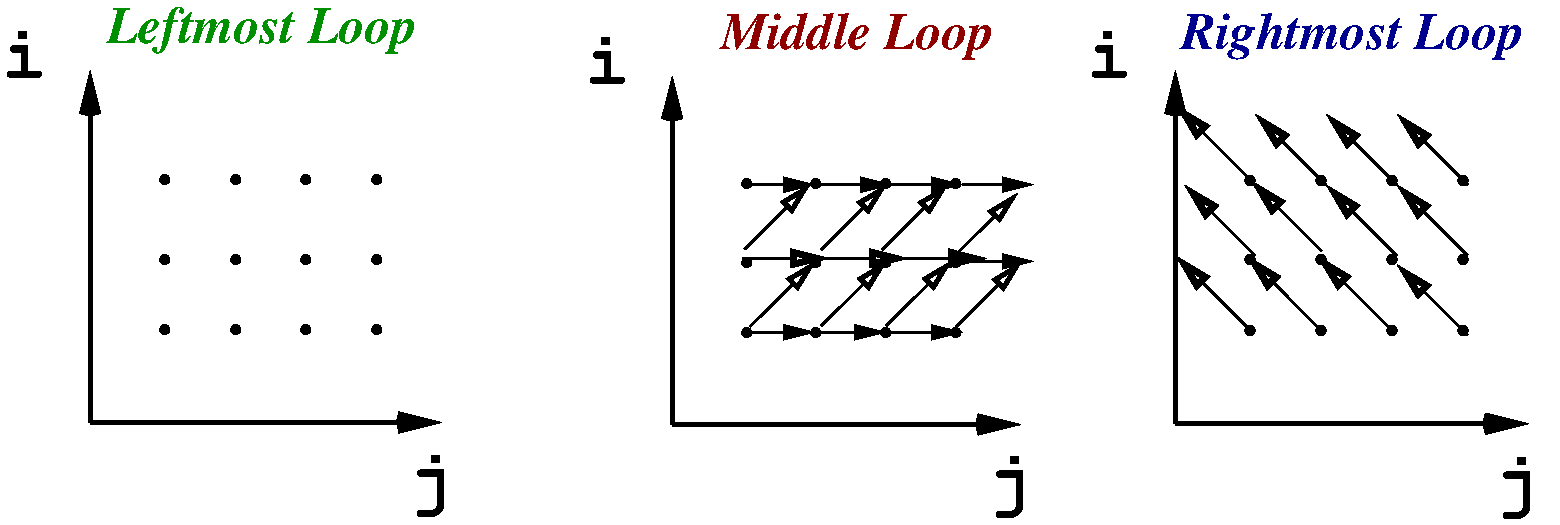
\includegraphics[width=90ex]{Figures/L5/LoopDeps}
\caption{Graphical representation of the dependencies for the three running examples shown in \cref{fig:data-dep-running-eg}; the $x$ and $y$ axis correspond to the index of the inner and outer \lstinline{do} loop, respectively.}
\label{fig:dep-graph}
\end{figure} 

A graphical representation of the dependencies of the three running code
examples is shown in \cref{fig:dep-graph}.   They can be intuitively inferred 
as follows:
\begin{itemize}
    \item For the loop in \cref{fig:data-dep-running-eg}(a), different
loop-nest iterations $(i_1,j_1)$ and $(i_2,j_2)$ necessarily read and write 
different array elements {\tt A[$j_1,i_1$]} and {\tt A[$j_2,i_2$]}.
This is because the assumption was that $(i_1,j_1) \neq (i_2,j_2)$, 
hence it cannot be that both $i_1 = i_2$ and $j_1 = j_2$. As such,
the representation of dependencies should be a set of points (no arrows), 
meaning that all dependencies actually occur inside the same 
iteration---in fact they are anti intra-iteration dependencies (WAR) 
because {\tt A[j,i]} is read first and then {\tt A[j,i]} is written 
inside the same iteration.
    \item For the loop in \cref{fig:data-dep-running-eg}(b) we reason
        individually for statements $S_1$ and $S_2$ because each
        statement accesses (one) array {\tt A} and {\tt B}, respectively:
        \begin{itemize}
            \item[$S_1:$] Let's take an iteration, say $(i_1=2, j_1=3)$,
                which \emph{reads} element {\tt A[$j_1$-1,$i_1$-1] = A[2,1]}. 
                Since an iteration $(i,j)$ always writes the element 
                {\tt A[i,j]}, we can reason that iteration $(i_2=1, j_2=2)$ 
                will \emph{write} the same element {\tt A[2,1]}. 
                It follows that we have discovered a true (RAW) dependency, 
                depicted in the figure with and arrow, from the source 
                iteration $(i_2=1, j_2=2)$---which writes {\tt A[2,1]}---to 
                the sink iteration $(i_1=2, j_1=3)$---which reads {\tt A[2,1]}. 
                This is because iteration $(1,2) < (2,3)$ according to the 
                lexicographical ordering, and as such, the read happens after 
                the write (RAW) in program order. One can individually reason
                for each point of the iteration space and fill it with oblique,
                forward-pointing arrows denoting true dependencies between 
                different instances of statement $S_1$ 
                (executing in different iterations).
            \item[$S_2:$] Following a similar rationale, iteration $(i_1=2, j_1=3)$
                \emph{reads} element {\tt B[$j_1$-1,$i_1$] = B[2,2]}, and 
                iteration $(i_2=2, j_2=2)$ \emph{writes} element {\tt B[2,2]}.
                It follows that we have discovered a true (RAW) dependency
                with source $(i_2=2, j_2=2)$ and sink $(i_1=2, j_1=3)$,
                because $(2,2) < (2,3)$ in lexicographic ordering.
                Since $i_1=i_2$ we depict the arrow parallel with the
                horizontal axis (that depicts values of $j$). One can
                fill in the rest of the iteration space with horizontal arrows. 
        \end{itemize}

    \item For the loop in \cref{fig:data-dep-running-eg}(c) we reason in
        a similar way: take iteration $(i_1=2, j_1=3)$ that \emph{reads}
        element {\tt A[2-1,3+1] = A[1,4]}. This element is \emph{written}
        by iteration $(i_2=1,j_2=4)$. It follows that we have discovered
        a true (RAW) from source $(i_2=1,j_2=4)$ to sink 
        $(i_1=2, j_1=3)$---because the read happens in iteration $(2,3)$
        which comes after the write in iteration $(1,4)$,
        i.e., $(1,4) < (2,3)$.  Thus, one can fill in the iteration
        space with oblique, backward-pointing arrows, denoting true dependencies
        between instances of $S_1$ executing in different iterations.
\end{itemize}

We have applied above a human type of reasoning and, as a result, we
have a graphical representation of all dependencies. However, such a reasoning
is not suitable for compiler-based automation because (i) the loop counts
are statically unknown---they depend on the dataset---hence one cannot 
possibly represent an arbitrary large iteration space, and, more importantly,
(ii) even if the loop counts would be statically known it is still inefficient 
to maintain and work with all this pointwise information. 

A representation that promotes compiler reasoning should succinctly capture 
the pattern that is multiplexed in the figure. Intuitively and imprecisely,
for \cref{fig:data-dep-running-eg}(a) the pattern would correspond to a point,
for \cref{fig:data-dep-running-eg}(b) it would correspond to two 
arrows---one oblique and one horizontal forward pointing arrows---and
for \cref{fig:data-dep-running-eg}(c) it would correspond to an
oblique, backward-pointing arrow.
%
These patterns are formalized by introducing the notion of direction vectors,
which are defined below.

\begin{mydef}[Dependency-Direction Vector]\label{Dep-Dir-Vect}
$\mbox{ }$\\
Assume there exists a dependency with source $S1$ in iteration $\ov{k}$
to sink $S2$ in iteration $\ov{l}$ ($\ov{k}\leq\ov{l}$).
We denote by {\tt m} the depth of the loop nest, we use $i$ to range
from {\tt $0,\ldots,$m-1}, and we denote by $x_i$ the $i^{th}$
element of some vector $\ov{x}$ of length {\tt m}.

The \emph{direction vector} between the instance of statement $S_1$ 
executed in some source iteration $\ov{k}$and statement $S_2$ executed
in sink iteration $\ov{l}$ is denoted by $\ov{D}(S_1\in\ov{k},S2\in\ov{l})$,
and corresponds to a vector of length {\tt m}, whose elements are defined as:
\[
D_i(S_1\in\ov{k},S_2\in\ov{l})=
    \begin{cases} 
        \mbox{\tt<} \ \ \ \ \mbox{\tt if it is provably that} ~~k_i ~<~ l_i,\\
        \mbox{\tt=} \ \ \ \ \mbox{\tt if it is provably that} ~~k_i ~=~ l_i,\\
        \mbox{\tt>} \ \ \ \ \mbox{\tt if it is provably that} ~~k_i ~>~ l_i,\\
        \mbox{\tt{}*} \ \ \ \ \mbox{\tt if}~k_i ~\mbox{\tt{}and}~ l_i~\mbox{are statically uncomparable.}\\
    \end{cases}
\]
\end{mydef}

The first three cases of the definition above assume that the ordering
relation between $k_i$ and $l_i$ can be statically derived in a generic
fashion (for any source $k_i$ and $l_i$); if this is not possible than 
we use the notation {\tt *} which \emph{conservatively} assumes that any 
directions may be possible---i.e., star should be understood as 
simultaneous existence of all {\tt <, =, >} directions. For example,
the loop
\begin{lstlisting}[mathescape=true]
do i = 0, N-1
$S_1:$  A[ X[i] ] = ...
enddo
\end{lstlisting}\vspace{-2ex}
would result in direction vector {\tt[*]} corresponding to a potential
output dependency (WAW), because the write access to {\tt A[ X[i] ]} is 
statically unanalyzable---for example under the assumption that 
the indirect array {\tt X} is part of the dataset---and, as such, 
all direction vectors may possibly hold between various pairs of 
instances of statement $S_1$ executed in different iterations.

We also remark that the symbols {\tt <, =, >} are \emph{not} connected at
all to the type of the dependency, e.g., true (RAW) or anti (WAR) dependency. 
The type of the dependency is solely determined by the operation of the
source and that of the sink: If the source is a write statement and the 
sink is a read then we have a true (RAW) dependency; if the source is a 
read and the sink is a write then we have an anti (WAR) dependency;
if both source and sink are writes then we have an output (WAW) dependency.  

The meaning of the symbol {\tt>} at some position $i$ is that
the source iteration at loop-level $i$ is greater than the sink
iteration at loop-level $i$. This case is possible, for example
the code in \cref{fig:data-dep-running-eg}(c) shows a dependency
with source iteration $(1,4)$ and sink iteration $(2,3)$. At the
level of the second loop, we have $4 > 3$ hence the direction
is {\tt >} but still the source iteration is less than the sink
iteration $(1,4) < (2,3)$ because of the first loop level.
This observation leads to the following corollary:

\begin{mycorol}[Direction Vector Legality]\label{Leg-Dir-Vect}
$\mbox{ }$\\
A direction vector is legal (well formed), if filtering out 
the {\tt =} entries does \emph{not} result in a leading {\tt>}
symbol. This would mean that a current iteration depends on
a future iteration, but depending on a future event is (considered)
impossible, and as such illegal.
\end{mycorol}

It remains to determine the sort of automatic reasoning 
(think compiler reasoning) that can be applied to compute
the direction vectors for the code examples in 
\cref{fig:data-dep-running-eg}:
\begin{description}
    \item[\cref{fig:data-dep-running-eg}(a):] dependencies
        can occur only between instances of statement $S_1$,
        executed in different (or the same) iterations.
        We recall that, by the definition of dependency,
        the two (dependent) iterations must access the same 
        element of {\tt A} and at least one iteration should 
        perform a write. 
        Since statement $S_1$ performs a read and a write to
        elements of array {\tt A}, two kinds of dependencies
        may occur:
    \begin{description}
        \item[WAW:] an output dependency may be caused by
        two write accesses in two different iterations,
        denoted $(i_1,j_1)$ and $(i_2,j_2)$. The written
        element is thus {\tt A[j$_1$,i$_1$]}, which must
        be the same as {\tt A[j$_2$,i$_2$]} for a dependency
        to exist. This results in
        the system of equations $\begin{cases}i_1 = i_2\\j_1 = j_2\end{cases}$
        which leads to direction vector {\tt[=,=]}.
        Hence, an output dependency from $S_1$ to $S_1$ 
        happens in the same iteration, but statement $S_1$
        executes only one write access in the same iteration.
        The conclusion is that no output dependency can occur,
        hence the direction vector is discarded.
        \item[RAW:] a true or anti dependency---we do not 
        know yet which---will be caused by the read access from 
        {\tt A} and the write access to {\tt A} in different 
        (or same) iterations. Remember that a statement such
        as {\tt A[j,i] = A[j,i] + 3} actually corresponds to
        three hardware instructions, hence either an inter- or
        an intra-dependency will necessarily occur.
        Assume some iteration $(i_1, j_1)$ reads from 
        {\tt A[j$_1$,i$_1$]} and iteration $(i_2,j_2)$ 
        writes to {\tt A[j$_2$,i$_2$]}.
        In order for a dependency to exist, the memory location
        of the read and write must coincide; this results
        in the system of equations: 
        $\begin{cases}i_1 = i_2\\j_1 = j_2\end{cases}$
        from which we can derive the direction vector:
        {\tt[=,=]}. This implies that the dependency happens
        in the same iteration, hence it is an intra-dependency.
        Furthermore, since the write follows the read in the
        instruction order of an iteration, this is an anti 
        dependency (WAR).
    \end{description}
    \item[\cref{fig:data-dep-running-eg}(b):] dependencies
        may possibly occur between instances of statement $S_1$
        and between instances of statement $S_2$. The case of
        output dependencies is disproved by a treatment similar
        to the bullet above. It remains to examine the dependency
        caused by a read and a write in different instances of
        $S_1$ and $S_2$, respectively:
    \begin{description}
        \item[$S_1$:] assume iteration $(i_1,j_1)$ and iteration
        $(i_2,j_2)$ reads from and writes to the same element of 
        {\tt A}, respectively. Putting this in equation results in
        the system: $\begin{cases}i_1-1 = i_2\\j_1-1 = j_2\end{cases}$,
        which necessarily means that $i_1 > i_2$ and $j_1 > j_2$.
        However, we do not know yet which iteration is the source
        and which is the sink. Assuming that $(i_1, j_1)$ is the
        source results in the direction vector {\tt[>,>]}, which is
        illegal by \cref{Leg-Dir-Vect}, because a direction
        vector cannot start with the {\tt>} symbol. It follows
        that our assumption was wrong: $(i_2, j_2)$ is the source
        and $(i_1, j_1)$ is the sink, which means that this is
        a cross-iteration (inter-iteration) true dependency
        (RAW)---because the sink iteration reads the element 
        that was previously written by the source iteration---and
        its direction vector is {\tt[<,<]}.
        \item[$S_2$:] a similar rationale can be applied to
        determine that two instances of $S_2$ generate
        a true cross-iteration dependency (RAW), whose
        direction vector is {\tt[=,<]}. In short, using the
        same notation results in the system of equations  
        $\begin{cases}i_1 = i_2\\j_1-1 = j_2\end{cases}$,
        hence the source must be $(i_2,j_2)$ and the sink
        must be $(i_1,j_1)$ and the direction vector is {\tt[=,<]}.
    \end{description}
    \item[\cref{fig:data-dep-running-eg}(c):] dependencies
        may possibly occur between instances of statement $S_1$.
        Assume iteration $(i_1,j_1)$ and $(i_2,j_2)$ reads from 
        and writes to the same element of {\tt A}, respectively.
        Putting this in equation results in the system
        $\begin{cases}i_1-1 = i_2\\j_1+1 = j_2\end{cases}$,
        which necessarily imply that $i_1 > i_2$ and
        $j_1 < j_2$. Choosing $(i_1,j_1)$ as the source
        of the dependency results in direction vector
        {\tt[>,<]}, which is illegal because it has
        {\tt >} as the first non-{\tt=} outermost symbol,
        as stated by \cref{Leg-Dir-Vect}. It follows that
        $(i_1,j_1)$ must be the sink and $(i_2,j_2)$
        must be the source, which results in the direction
        vector {\tt[<,>]}, which is legal. Since the source 
        writes and the sink reads, then we deal with a true 
        dependency (RAW). 
        Moreover since the direction vector
        indicates that the source iteration is strictly 
        less than the sink iteration, this is also a
        cross-iteration dependency.
\end{description}

\begin{mydef}[Dependency-Direction Matrix]\label{Dep-Dir-Mat}
A direction matrix is obtained by stacking together the
direction vectors of all the intra- and cross-iteration
dependencies of a loop nest (i.e., between any possible
pair of write-write or read-read instruction instances).
\end{mydef}

In conclusion the direction matrices for the three running
code examples in \cref{fig:data-dep-running-eg} are:
\begin{description}
    \item[(a):] $\begin{cases}\mbox{\tt [=,=]}\end{cases}$
    \item[(b):] $\begin{cases}\mbox{\tt[<,<]}\\\mbox{\tt[=,<]}\end{cases}$
    \item[(c):] $\begin{cases}\mbox{\tt[<,>]}\end{cases}$
\end{description}
The following section will show how the legality of powerful code
transformations can be reasoned in a simple way in terms of 
direction vectors/matrices.
 

\subsection{Determining Loop Parallelism by Analyzing Direction Vectors}
\label{subsec:loop-par}

A loop is said to be parallel if its execution does not
cause any (true, anti or output) dependencies across
its iterations---the loop execution is assumed to be fixed
in a specific iteration of an (potentially empty) enclosing
loop context.

The following theorem states that a sufficient condition for
a loop to be parallel is that for all the elements in
the loop's corresponding direction-matrix column, it holds
that the element is either {\tt=} or there exists an
outer loop whose corresponding direction is {\tt<} (on that row).
In the latter case we say that the outer loop carries
all the dependencies of the inner loop, i.e., fixing
an iteration of the outer loop (think executing the outer
loop sequentially) would guarantee the absence of cross-iteration
dependencies in the inner loop.  

\begin{mytheo}[Parallel Loop]\label{Loop-Par}
$\mbox{ }$\\
We assume a loop nest denoted by $\ov{L}$, whose direction
matrix is denoted by $M$ and consists of $m$ rows.
{\em A sufficient condition} for a loop at depth $k$ in $\ov{L}$,
denoted $L_k$, to be parallel is that
$\forall i\in\{0,\ldots m-1\}~$ either $M[i,k]$ is equal
to {\tt=} or there exists an outer loop (at depth $q<k$)
such that $M[i,q]$ is equal to {\tt<}.
\emph{The proof} is left as an exercise.
\end{mytheo}

Theorem~\ref{Loop-Par} claims to give only a sufficient condition for 
loop parallelism because it assumes that symbols such as {\tt *}
may be part of the direction vector elements---we recall that
{\tt *} conservatively assumes that all directions {\tt <,=,>}
may be possible. If {\tt *} does not appear in the direction
matrix, then the condition becomes necessary and sufficient,
i.e., the loop is parallel if and only if $\ldots$.
Let us analyze the parallelism of each loop in our running
examples:
\begin{description}
\item[\cref{fig:data-dep-running-eg}(a):] The direction matrix
        is {\tt [=,=]}, hence by \cref{Loop-Par}, both loops
        in the nest are parallel because all the directions
        are equal to {\tt=}.
\item[\cref{fig:data-dep-running-eg}(b):] The direction matrix is
        $M = \begin{cases}\mbox{\tt[<,<]}\\\mbox{\tt[=,<]}\end{cases}$,
        hence neither the outer nor the inner loop can 
        be proven parallel by \cref{Loop-Par}. In the former case
        this is because $M[0,0]$ is equal to {\tt<} and there is 
        no other outer loop to carry dependencies. In the latter 
        case this is because $M[1,1]$ is equal to {\tt<} and the 
        outer loop for that row has direction 
        {\tt=} (instead of {\tt<}, which would have been necessary 
        to carry the dependencies of the inner loop).
\item[\cref{fig:data-dep-running-eg}(c):] The direction matrix is
        {\tt[<,>]}, which means that the outer loop is not 
        parallel---because it has a leading {\tt<} direction)---but 
        the {\em inner loop is parallel}
        because the outer loop starts with {\tt<} on the only row
        of the direction matrix, and, as such, it carries all the
        dependencies of the inner loop.   To understand what this
        means, take a look again at the actual code in
        \cref{fig:data-dep-running-eg}(c): let us fix the outer
        iteration number to some value {\tt i}. Then the read accesses
        always refer to row {\tt i-1} of matrix {\tt A} and the write 
        accesses always refer to row {\tt i} of {\tt A}; hence a
        cross-iteration dependency cannot happen in the inner loop 
        because no matter of the value of {\tt j}, the read and write
        statement instances cannot possibly refer to the same  
        location of {\tt A}.
\end{description}

\subsection{Loop Interchange: Legality and Applications}
\label{subsec:loop-interch}

Direction vectors are not used only for proving the parallel
nature of loops, but they can also enable powerful code
restructuring techniques. For example they can be 
straightforwardly applied to determine whether it is safe
to interchange two loops in a perfect loop nest\footnote{
A perfect loop nest is a nest in which any two loops at
consecutive depth levels are not separated by any other 
statements; for example all loop nests in 
\cref{fig:data-dep-running-eg} are perfectly nested.
}---which may result in better locality and even in changing
an inner loop nature from dependent (sequential) to parallel.

The following theorem gives a sufficient condition for the
legality of loop interchange---i.e., for the transformation 
to result in code that is semantically equivalent to the original one.


\begin{mytheo}[Legality of Loop Interchange]\label{Loop-Interch}
$\mbox{ }$\\
A sufficient condition for the legality of interchanging 
two loops at depth levels $k$ and $l$ in a perfect nest 
is that interchanging columns $k$ and $l$ in the direction 
matrix of the loop nest {\em does not result} in a (leading)
{\tt>} direction as the leftmost non-{\tt=} direction 
of any row.
\end{mytheo}

The theorem above shows that the legality of loop interchange
can be determined solely by inspecting the result of permuting
the direction matrix in the same way as the one desired for loops.
For the rationale related to why a row-leading {\tt>} direction
is illegal, we refer the reader to \cref{Leg-Dir-Vect}: a non-{\tt=}
leading {\tt>} direction would correspond to depending on something
that happens in the future: this currently seems impossible in our
universe, and as such it signals an illegal transformation.
%
The following corollary can be easily derived from \cref{Loop-Interch}:

\begin{mycorol}[Interchanging a Parallel Loop Inwards]\label{Par-Loop-Interch}
$\mbox{ }$\\
In a perfect loop nest, it is always safe to interchange a 
{\em parallel loop} inwards one step at a time (i.e., if the
parallel loop is the $k^{th}$ loop in the nest then one can
always interchange it with loop $k+1$, then with loop $k+2$, etc.).
\end{mycorol}

The corollary says that if we somehow know the parallel nature
of a loop, then we can safely interchange it in the immediate inward 
position, without even having to build the dependence-direction matrix.
For example, \lstinline{map} operations have inherently parallel
semantics, and, as such, one can freely interchange inwards the
loops semantically corresponding to \lstinline{map} operations
(as long as the counts of the inner loops in the nest do not
depend on the index of the \lstinline{map}-like loop).

Let us analyze the legality of loop interchange for the three loop 
nests of our running example:
\begin{description}
\item[\cref{fig:data-dep-running-eg}(a):] The direction matrix
        is {\tt [=,=]} and, as such, it is legal to interchange
        the two loops, because it would result in direction
        matrix {\tt[=,=]}. Moreover applying loop interchange
        in this case is highly beneficial because it
        \textbf{\em optimizes locality of reference} (in a CPU setting): the 
        loop of index {\tt i} appears in the innermost position 
        after the interchange, which optimally exploits spatial 
        locality for the write and read accesses to {\tt A[j,i]}.
\item[\cref{fig:data-dep-running-eg}(b):] The direction matrices are
        $M = \begin{cases}\mbox{\tt[<,<]}\\\mbox{\tt[=,<]}\end{cases}$
        and
        $M^{intchg} = \begin{cases}\mbox{\tt[<,<]}\\\mbox{\tt[<,=]}\end{cases}$
        before and after interchange, respectively. 
        It follows that the loop interchange is legal---because 
        $M^{intchg}$ satisfies \cref{Loop-Interch}---and 
        it also optimizes spatial locality (as before).
        What is interesting about this example is that after the 
        interchange, \textbf{\em the innermost loop has become parallel},
        by \cref{Loop-Par}, because the outer loop caries
        all dependencies---the direction column corresponding to the
        outer loop consists only of {\tt<} directions.
\item[\cref{fig:data-dep-running-eg}(c):] The direction matrix is
        {\tt[<,>]} and \textbf{\em interchanging the two loops is illegal}
        because the direction matrix obtained after the interchange
        {\tt[>,<]} starts with a {\tt>} direction; this would
        mean that the current iteration depends on a future iteration,
        which is impossible, hence the interchange is illegal.
\end{description}

\subsection{Loop Distribution: Legality and Applications}
\label{subsec:loop-distrib}

This section introduces a transformation, named loop 
distribution, that refers to the manner in which a loop can 
be safely distributed across its statements. 
Potential benefits are:
\begin{itemize}
    \item loop distribution provides the bases for performing 
        vectorization:
        the innermost loop is distributed across its TAC statements,
        and then the distributed loops are chunked (stripmined) 
        by a factor that permits utilization of processor's vector 
        instructions.
    \item loop distribution may enhance the degree of
        parallelism that can be statically mapped to the 
        hardware, in a similar way in which it has been 
        applied for flattening in \cref{subsec:flatten-simple-eg}.
        There, a \lstinline{map} was distributed across its
        statements such as to create perfect nests of parallel
        constructs, which are then flattened by applying
        corresponding re-write rules. 
\end{itemize}

Loop distribution requires the construction of the dependency
graph, which is defined below.

\begin{mydef}[Dependency Graph]\label{Dep-Graph}
$\mbox{ }$\\
A dependency graph of a loop is a directed graph in which 
the nodes correspond to the statements of the loop nest and the
edges correspond to dependencies. An edge is directed (points) 
from the source to the sink of the dependency, and is annotated
with the direction corresponding to that dependence. 

In the case when the loop contains another inner loop, then 
the inner loop is represented as a single statement that conservatively 
summarizes the behavior of all the statements of the inner loop.
\end{mydef}

The dependency graph of a loop can be used to characterize its
parallel behavior:
\begin{mytheo}[Dependency Cycle]\label{Dep-Cycle}
$\mbox{ }$\\
A loop is parallel {\em if and only if} its dependency graph
does not have cycles.
\end{mytheo}
If the loop contains a cycle of dependencies, then it necessarily
exhibits at least a cross iteration dependency (needed to form 
the cycle), and thus the loop is not parallel.  The following
theorem specifies how the transformation can be implemented:

\begin{mytheo}[Loop Distribution]\label{Loop-Distrib}
$\mbox{ }$\\
Distributing a loop across its statements can be performed
in the following way:
\begin{itemize}
    \item[1.] The dependency graph corresponding to the target loop
        is constructed.
    \item[2.] The graph is decomposed into strongly-connected components 
            (SCCs)\footnote{
            A graph is said to be strongly connected if every vertex 
            is reachable from every other vertex, i.e., a cycle.
            It is possible to find the strongly-connected components
            of an arbitrary directed graph in linear time $\Theta(V+E)$,
            where $V$ is the number of vertices and $E$ is the number of
            edges.
        }, and a new graph $G'$ is formed in which the SCCs are nodes. 
    \item[3.] The loop can be safely distributed across its strongly-connected
        components, in the graph order of $G'$.
        Assuming a number $k$ of SCCs, this means that the result of the
        transformation will be $k$ loops, each containing the statements
        of the corresponding SCC. Inside an SCC, the statements remain in
        program order, but the distributed loops are ordered according to
        $G'$. 
    \item[4.] Array expansion must be performed for the variables that
        \begin{itemize}
            \item are either declared inside the loop or overwritten
                in each iteration (output dependencies), \textbf{\em and}
            \item are used in at least two strongly-connected components.
        \end{itemize} 
\end{itemize}
\end{mytheo}

The theorem above says that the statements that are in a dependency 
cycle must remain in (form) one loop (which is sequential by 
\cref{Dep-Cycle}). As such, the loop can be distributed across
groups of statements corresponding to the strongly connected 
components (SCC) of the dependency graph. If the graph has only one
SCC than it cannot be distributed.  The resulting distributed loops
are written in the order dictated by the graph of SCCs. 
%
We demonstrate \cref{Loop-Distrib} on the simple code example presented 
below:
\begin{lstlisting}[mathescape=true]
forall i = 2, N
$S_1:$  A[i] = B[i-2] ...
$S_2:$  B[i] = B[i-1] ...
endfor
\end{lstlisting}\vspace{-2ex}

The code has two dependencies:
\begin{description}
    \item[$S_2\to S_1$:]  In order for a dependency on {\tt B} to exist
        the read from {\tt B} in iteration $i_1$ of $S_1$ and 
        the write to {\tt B} in iteration $i_2$ of $S_2$ must refer
        to the same location. Hence {\tt i$_1$-2 = $i_2$}, which means
        {\tt i$_1$ > i$_2$}, hence $S_2$ is the source, $S_1$ is the
        sink and the direction vector is {\tt[<]};
    \item[$S2\to S2$:] similarly, there is a dependency between the
        read from {\tt B} in $S_2$ and the write to {\tt B} in $S_2$
        of direction vector {\tt[<]}.   
\end{description}

The dependency graph is thus:

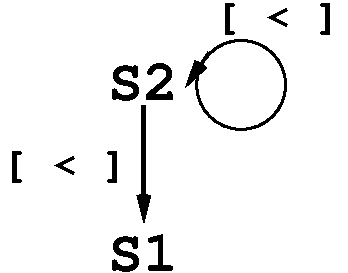
\includegraphics[height=15ex]{Figures/L5/LoopDistr}

\noindent and it exhibits two strongly-connected components:
one formed by statement $S_2$ and one formed by statement $S_1$.
Loop distribution results in the following restructured code:
\begin{lstlisting}[mathescape=true]
forall i = 2, N
$S_2:$  B[i] = B[i-1] ...
endfor
forall i = 2, N
$S_1:$  A[i] = B[i-2] ...
endfor
\end{lstlisting}\vspace{-2ex}
in which, according to the graph order, the loop corresponding to
statement $S_2$ appears before the one corresponding to statement
$S_1$. Please notice that this does not match the program order 
of statements $S_1$ and $S_2$ in the original program. Please also 
notice that the first loop is {\em not} parallel because the SCC 
consisting of $S_2$ has a (dependency) cycle, but the second loop 
is parallel because the SCC corresponding to $S_1$ does not have 
cycles.

One can notice that if a loop is parallel then it can be straightforwardly
distributed across its statements in program order because:
\begin{itemize}
    \item by \cref{Dep-Cycle}, the loop dependency graph have no
            cycles and thereby each statement is a strongly connected
            component; 
    \item the program order naturally respects all dependencies.
\end{itemize}

\begin{mycorol}[Parallel Loop Distribution]\label{Par-Loop-Distr}
$\mbox{ }$\\
A parallel loop can be directly distributed across each one of
its statements. The resulted loops appear in the same order in 
which their corresponding statements appear in the original loop.
\end{mycorol}

In fact, this is the theorem that provides the safety rationale
for the \lstinline{map} distribution used to perform flattening
in  \cref{subsec:flatten-simple-eg} (under the trivial observation
that a \lstinline{map} is a parallel loop).

Finally, it remains to demonstrate array expansion, mentioned
in the fourth bullet of \cref{Loop-Distrib}. Assume the slightly
modified code:
\begin{lstlisting}[mathescape=true]
float tmp;
forall j = 0, N-1
    i = j + 2
$S_1:$  tmp  = 2 * B[i-2]
$S_2:$  A[i] = tmp
$S_3:$  B[i] = tmp + B[i-1]
endfor
\end{lstlisting}\vspace{-2ex}
Statements $S_1$ and $S_3$ are in a dependency cycle, because
there is a dependency $S_3\to S_1$ with direction {\tt<} caused
by the write to and the read from array {\tt B}, and a dependency 
$S_1\to S_3$ with direction {\tt=} caused by {\tt tmp}.
Statement $S_2$ is not in a dependency cycle, but there is a
dependency $S_1\to S_2$, and hence its distributed loop
should follow the distributed loop containing $S_1$ and $S_3$. 
If we do not perform array expansion, the distributed code:

\begin{lstlisting}[mathescape=true]
float tmp;
forall j = 0, N-1
    i = j + 2
$S_1:$  tmp  = 2 * B[i-2]
$S_3:$  B[i] = tmp + B[i-1]
endfor
forall j = 0, N-1
    i = j + 2
$S_2:$  A[i] = tmp
endfor
\end{lstlisting}\vspace{-2ex}
\noindent does not respect the semantics of the original program
because the second loop uses the same value of {\tt tmp}---the one
set by the last iteration of the first loop---while the original
loop writes and then reads a different value of {\tt tmp} for 
each iteration. It follows that we must perform array expansion
for {\tt tmp}, which means that we must expand it with an array 
dimension equal to the loop count and replace its uses with
corresponding indexing expressions of the expanded array. 
This results in the following {\em correct} code:
\begin{lstlisting}[mathescape=true]
float tmp[N];
forall j = 0, N-1
    i = j + 2
$S_1:$  tmp[j]  = 2 * B[i-2]
$S_3:$  B[i] = tmp + B[i-1]
endfor
forall j = 0, N-1
    i = j + 2
$S_2:$  A[i] = tmp[j]
endfor
\end{lstlisting}\vspace{-2ex}

Array expansion requires to normalize the loop first---this means
rewriting the loop such as its index starts from $0$ and increases
by $1$ each iteration. This is why we have not written our example
as \lstinline{for i = 2, N+1}.

\enlargethispage{\baselineskip}

\subsection{Eliminating False Dependencies (WAR and WAW)}
\label{subsec:false-dep-elim}

Anti and output dependencies are often referred to as {\em false}
dependencies because they can be eliminated in most cases by
copying or privatization operations:
\begin{itemize}
    \item Cross-iteration anti dependencies (WAR) typically
        correspond to a read from some original element of 
        the array---whose value was set before the start of 
        the loop execution---followed by an update to that 
        element in a later iteration.  As such, this dependency
        can be eliminated by copying (in parallel) the target
        array before the loop and rewriting the offending
        read access inside the loop such that it refers
        to the copy of the array.\smallskip

    \item Cross-iteration output dependencies (WAW) can be
        eliminated by a technique named privatization (or renaming), 
        whenever it can be determined that {\em every read access} 
        from a scalar or array location {\em is covered by an
        update} to that scalar or memory location that was
        previously performed {\em in the same iteration}. 
        Semantically, privatization moves the declaration of the
        offending variable inside the loop, because it has been
        already determined that the read/used value was produced
        earlier in the same iteration.\smallskip

    \item Reasoning based on direction vectors is limited to 
        relatively simple loop nests; for example it is difficult 
        to reason about privatization by means of direction vectors.
\end  {itemize}

\subsubsection{Eliminating WAR Dependencies by Copying}
$\mbox{ }$\\

Consider the simple {\tt C} code below which rotates an array in
the right dimension by one:
\begin{lstlisting}[mathescape=true]
float tmp = A[1];
for (int i=0; i<N-1; i++) {
    A[i] = A[i+1]; -- $S_1$   
}
A[N-1] = tmp;
\end{lstlisting}\vspace{-2ex}
The loop exhibits a cross-iteration anti dependency (WAR)
$S_1\to S_1$ (with direction vector ${\tt[<]}$), and, as 
such, it is not safe to execute it in parallel. However, 
one can observe that the reads from {\tt A} inside the loop
correspond to the original elements of {\tt A} before
the loop, because they are rewritten in a later iteration.
As such one can perform a copy of {\tt A} before the loop, 
and replace the read access inside the loop to operate on 
the copy of array {\tt A}. This preserves the original 
loop semantics and results in a parallel loop because
the read and write accesses operate on different arrays,
hence a dependency cannot occur. We present below the
OpenMP code, which is a popular parallel API for multicore 
hardware:
\begin{lstlisting}[mathescape=true]
float Acopy[N];
#pragma omp parallel for
for(int i=0; i<N; i++)} {
    Acopy[i] = A[i];
}
tmp = A[1];
#pragma omp parallel for
for (int i=0; i<N-1; i++) {
    A[i] = Acopy[i+1];
}
A[N-1] = tmp;
\end{lstlisting}\vspace{-2ex}
The code uses the {\tt\#pragma omp parallel for} annotation,
by which the programmer solemnly swears that the following
\lstinline{for} loop is actually parallel; if the programmer
breaks the vow then the parallel and sequential execution of
the code will give different results; the API does not provide
any guarantees about the absence of race-conditions. 
To compile with support for OpenMP annotation in {\tt gcc},
please use the {\tt-fopenmp} compilation flag. The number
of cores that are going to be used for parallel execution
can be set by environment variable {\tt OMP\_NUM\_THREADS}
for example by the command line {\tt\$export OMP\_NUM\_THREADS=8}
if you would like to utilize eight threads.

\newpage
\subsubsection{Eliminating WAW Dependencies by Privatization}
$\mbox{ }$\\

Consider the contrived and ugly looking {\tt C} code below:
\begin{lstlisting}[mathescape=true]
int i;
int A[M];
for(i=0; i<N; i++){
  for(int j=0, j<M; j++) { -- writes slice A[0:M-1]
    A[j] = (4*i+4*j) % M;                          -- $S_1$
  } 
  for(int k=0; k<N; k++) { -- reads A[j] where j$\in${0,$\ldots$M-1}
    X[i,k] = X[i,k-1] * A[ A[(2*i+k)%M] % M];      -- $S_2$
  }                        -- because % denotes modulus op 
}
\end{lstlisting}\vspace{-2ex}

Analyzing the cross-iteration dependencies of the outer loop,
one can observe that there are frequent output dependencies
$S_1\to S_1$ of all directions ({\tt *}), because, in 
essence, all elements of {\tt A} at indices $0\ldots M-1$
are (over)written in each iteration of the outer loop.
This also causes frequent cross-iteration WAR and RAW 
dependencies between $S_1$ and $S_2$ of all directions
{\tt *} because $S_2$ reads some of the values of 
{\tt A} which are written in $S_1$. The read access
is also statically unanalyzable because the index
into {\tt A} depends on a value of {\tt A} (i.e., 
it is an indirect-array access {\tt A[ A[...] ]}).  

It would thus seem that this is a hopeless case and parallel
execution is a pipe dream. Not so! Actually the rationale
of how to transform the outer loop into a parallel one
is quite simple.  One may observe that each iteration of
the outer loop writes the same indices of {\tt A}, namely
the ones belonging to the closed integral interval 
{\tt [0,M-1]}.   One may also observe that $S_2$ reads 
from {\tt A} elements whose indices necessarily belong to 
{\tt [0,M-1]}---due to the two modulus-{\tt M} operations. 
As such, one may conclude that any value
read in $S_2$ must have been produced in the same iteration
of the outer loop (in the inner loop enclosing $S_1$).

It follows that it is safe to rewrite the loop in the
following way:
\begin{itemize}
    \item[(1)] declare a new variable {\tt A'} of the same dimensions 
        as {\tt A} just inside the outer loop (or equivalently 
        perform array expansion of array {\tt A'} with a new outer
        dimension of size {\tt N}), and
    \item[(2)] replace all the uses of {\tt A} in the outer loop by
        uses of {\tt A'};
    \item the resulting loop is safe to execute in parallel
        because there can be no dependencies on {\tt A'} since
        each iteration uses a different array {\tt A'};
    \item[(3)] as a last step, after the parallel execution of
        the loop terminates, one must copy (in parallel)
        the elements produced by the last iteration of 
        the outer loop (i.e., {\tt A'[0,$\ldots$,M-1]} 
        back to {\tt A}.
\end{itemize}

The parallel OpenMP code that implements these steps is 
presented below:
\begin{lstlisting}[mathescape=true]
int A[M];
int i;
#pragma omp for lastprivate(i) lastprivate(A) 
for(i=0; i<N; i++) {
    for(int j=0, j<M; j++) {
        A[j] = (4*i+4*j) % M;
    }
    for(int k=0; k<N; k++) {
        X[i,k]=X[i,k-1] * A[ A[(2*i+k) % M] % M];
}   }
\end{lstlisting}\vspace{-2ex}
Declaring array {\tt A} as private (by {\tt private(A)}) would 
result in semantically performing steps (1) 
and (2) above. Declaring it as {\tt lastprivate(A)} instructs 
the OpenMP compiler to also perform step (3)---to copy back 
the privately-maintained result of {\tt A} of the last executing 
iteration into the globally-declared array {\tt A}.

Please also note that the OpenMP execution will not allocate
a new {\tt A'} for each iteration of the outer loop---this is 
actually equivalent to performing array expansion which is also
applicable here---but instead it will {\em allocate a copy of 
{\tt A} for each active thread}, thus significantly reducing 
the memory footprint and/or the number of (de)allocations.
 
We also remark that {\tt i} is also declared
{\tt lastprivate}---because its value might be needed after
the loop. Semantically, {\tt i} generates true cross-iteration
dependencies, and we have said that those are difficult to eliminate
in general, because they correspond to algorithmic properties.
The technique by which variables such as {\tt i}\footnote{which are
incremented by same ammount in each iteration of the loop} can 
be resolved is not actually privatization (OpenMP uses the wrong 
nomenclature here), but rather induction-variable recognition and 
substitution.

We conclude by repeating that privatization can be applied whenever
one can prove that every read access in an iteration is covered by 
a previously-performed write access in the same iteration. 
Privatization can be implemented by performing either array 
expansion or moving the declaration of the target variable from
outside to inside the loop. However, it saves memory to allocate
the private copy per active thread rather than per iteration,
which is what OpenMP is doing. In the GPU context (CUDA) it is
likely that you would have to implement privatization by 
array expansion.

\subsection{Recognizing Data-Parallel Operators Hidden in Sequential, Imperative Code}
\label{subsec:soacs-in-imp-code}

Section~\ref{sec-nested-par} has argued that programs written with parallelism
in mind should be built---or at least be reasoned about---in terms of a nested
composition of operators that have inherently parallel semantics, such 
as \lstinline{map}, \lstinline{reduce}, \lstinline{scan}, \lstinline{filter}. 
%
An important question is then ``How can one identify and extract such 
operators from a sequential (legacy) code base?''. 
%
This section attempts to provide an (incomplete) answer to this
question, in the simpler case when the hardware is a multi-core 
machine.

\subsubsection{Recognizing Reduce Operators}
\label{subsubsec:reduce-imp}
$\mbox{ }\\$ 

We say that a (scalar) variable {\tt x} in a target loop is in a
reduce pattern if and only if all the statements in which {\tt x}
appears are of the form {\tt x = x $\odot$ exp}, where {\tt x} 
does not appears in {\tt exp} and $\odot$ is an associative operator.
Such statements naturally raise cross-iteration true dependencies
(RAW). However, these dependencies can be resolved in a simple
way, by:
\begin{itemize}
    \item[(1)] privatizing {\tt x}, which is initialized with
        the neutral element for each thread;
    \item[(2)] executing the loop in parallel, such that each
        thread computes its own partial value for {\tt x},
        corresponding to the iterations it executes;
    \item[(3)] reducing the partial values of {\tt x} across
        processors by a reduction tree---or sequentially
        if the number of cores is small, which is the case of 
        multicores;
    \item[(4)] adding to the result the value of {\tt x}
        from before the loop.
\end{itemize}
This is a simple technique; we point to the work of Lu and 
Mellor-Crummey for advanced compiler algorithms for identifying 
and optimizing reductions~\cite{ExtRed}.

In fact, the procedure above refers to parallelizing a
\lstinline{map-reduce} composition---see list homomorphism
\cref{sec:ListHom}---in which, intuitively, the various
{\tt exp}s for a given iteration are obtained and added 
together semantically by a \lstinline{map} operation,
and then reduced across iterations by {\tt $\odot$}. 
When using OpenMP, one must remember that OpenMP supports
a fixed (small) set of reduce operators, such as integral 
or float addition, multiplication, and perhaps taking the 
maximum/minimum; it is not possible to work with an 
arbitrary operator.
Please also notice that the same kind of rationale can be 
used in principle for the case when the variable is of an 
array type---for example a reduce with vectorized 
addition---except that it will be more difficult to recognize 
the operator, since this will likely be implemented as a loop.

We demonstrate the case of reduction on the following code,
where we aim to parallelize the outer loop:
\begin{lstlisting}[mathescape=true]
int i, j;
float x = 6.0;
for(i=1; i<N; i++) {
    for(j=1; j<N; j++) {
        if ( A[i,j] >= 2.0 )    x += 2*A[i,j-1];
        else if( A[i,j] > 0.0 ) x += A[i-1,j+1];
    }
    if (i % (j+1) == 3) 
        x += A[i,i];
}
\end{lstlisting}

One may observe that all uses of variable {\tt x} inside
the outermost loop respect the reduction pattern, i.e.,
{\tt x} is only used inside reduction statements. The
outer loop can be parallelized under OpenMP by placing 
the following reduction annotation just before
the outermost loop:\\
{\tt\#pragma omp parallel for reduction(+:x) private(i,j)}\\
and the program can be compiled with {\tt gcc} by using
the {\tt -fopenmp} flag.

The above imperative program is semantically equivalent
with the following Futhark program
\begin{lstlisting}[mathescape=true]
let x_ini = 6.0
let xs = map (+1) (iota (N-1)) |> 
         map (\i ->
                let exps = map (+1) (iota (N-1)) |>
                    map (\j -> let a = A[i,j] in
                               if a >= 2.0   then 2*A[i,j-1]
                               else if a > 0 then A[i-1,j+1]
                               else 0.0
                        )
                let e = reduce (+) 0.0 exps
                let e' = if (i % (j+1) == 3) then A[i,i] else 0.0
                in  e + e'
             )
let x = (reduce (+) 0 xs)
in x_ini + x
\end{lstlisting}\vspace{-2ex}
in which, if desired, the inner parallelism can be either exploited
or sequentialized.

Finally, we remark that imperative code patterns might be
deceiving, for example a reduction pattern might actually
turn to be a \lstinline{map} or a \lstinline{scatter}.
For example, in the code below:
\begin{lstlisting}[mathescape=true]
for(int i=0; i<N; i++)
   A[i] = A[i] + 2;
\end{lstlisting}\vspace{-2ex}
the statement that updates {\tt A[i]} respects the reduction
patterns, but the loop is actually a \lstinline{map} operation:
\lstinline{map (+2) A}.   This is a simple one, which is
easy to recognize. But what about the following one:
\begin{lstlisting}[mathescape=true]
for(int i=0; i<N; i++)
   A[ B[i] ] = A[ B[i] ] + 2;
\end{lstlisting}\vspace{-2ex}
The parallel semantics of the loop above actually depends on the
contents of indirect array {\tt B}, which is typically part of the
dataset, and thus statically unknown:
\begin{itemize}
    \item[(1)] if array {\tt B} does not contains duplicated 
        elements---i.e., $\forall i,j\in\{0\ldots N-1\}, \ i\neq j$ we have
        that {\tt B[$i$] $\neq$ B[$j$]} then the loop has the
        semantics of a \lstinline{scatter}:\\
        \lstinline{scatter A B <| map (\k -> A[k]+2) B}.
    \item[(2)] if array {\tt B} contains duplicated elements
        then the pattern is often called a generalized reduction
        on arrays (think histograms!), and can be executed in parallel 
        for example by using an atomic add operation---this of course 
        requires the operator to be associative and commutative, because
        the increments happen out of (the sequential) order.   
\end{itemize}
The test whether {\tt B} contains duplicates can also be performed
in parallel, and may guard the two different versions: a sufficient
condition for disproving duplicates is to check whether the values 
of {\tt B} are strictly monotonically increasing; this can be 
computed with the following efficient predicate:\\
\lstinline{map (+1) (iota (N-1)) |> map (\i -> B[i-1]<B[i]) |> reduce (&&) true}\\
A precise test is also possible by:\\
\lstinline{N == (scatter (replicate N 0) B (replicate N 1) |> reduce (+) 0)}\\
which first writes $1$ in an array of zeros at the indices of {\tt B}, then
sums the result and checks equality with the length of {\tt B}. Here the idea
is that if {\tt B} contains duplicates than at least two ones will be
written in the same location, and necessarily the sum will be smaller than
{\tt N}. However, this test is significantly slower (about $3\times$) than 
the monotonicity test. 


\subsubsection{Recognizing Scan Operators}
\label{subsubsec:scan-imp}
$\mbox{ }\\$ 

Scan operations are difficult to recognize by the compiler.
In principle, a loop-based implementation of \lstinline{scan}
will result in dependency cycle indicating a true dependency 
(RAW) of distance one---i.e., the current iterations depends 
on the result of the previous one. However not all such 
dependency pattern indicate \lstinline{scan} operations.
Furthermore, \lstinline{scan} can be sequentially implemented
in a multitude of forms, and as such they are difficult
pattern match. 

For example, the sequential, imperative code below:
\begin{lstlisting}[mathescape=true]
A[0] = B[0];
for(i=1; i<N; i++) {
    A[i] = A[i-1] + B[i];
}
\end{lstlisting}\vspace{-2ex}
is an inclusive scan: \lstinline{let A = scan (+) 0 B}.

The following loop:
\begin{lstlisting}[mathescape=true]
acc = 0;
for(i=0; i<N; i++) {
    acc = acc + i;
    A[i] = acc;
}
\end{lstlisting}\vspace{-2ex}
is also an inclusive scan, albeit applied to the {\tt iota N}
array: \lstinline{let A = scan (+) 0 (iota N)}.\bigskip

Let us conclude with a non-trivial example.
What kind of scan is represented by the code below?
\begin{lstlisting}[mathescape=true]
for(j=0; j<M; j++) 
    A[0,j] = B[0,j];

for(i=1; i<N; i++) {
    for(j=0; j<M; j++)
        A[i,j] = A[i-1,j] + B[i,j];
}
\end{lstlisting}\vspace{-2ex}
One can observe that, if we transpose matrices {\tt A} and {\tt B}, 
then the inner loop will resemble an inclusive scan, because it
will have the pattern: {\tt A$^{tr}$[j,i]=A$^{tr}$[j,i-1] + B[j,i]}.
It follows that the second loop nest (of depth {\tt 2}) actually 
performs a \lstinline{scan} on each column of the matrix {\tt B},
and the first single loop nest initializes the first element of
the column result with the corresponding element for {\tt B}.
The code is thus semantically equivalent to:\\
\lstinline{let A = transpose B |> map (scan (+) 0.0) |> transpose}


\subsubsection{Recognizing Filter Operators}
\label{subsubsec:filter-imp}
$\mbox{ }\\$ 

The natural implementation for \lstinline{let B = filter pred A} 
is by a loop which selectively adds elements to the result array 
whenever the predicate succeeds on the current array element:
\begin{lstlisting}[mathescape=true]
int k = 0;
for(i=0; i<N; i++) {
    if pred(A[i]) {
        B[k] = A[i];
        k = k + 1;
    }
}
\end{lstlisting}\vspace{-2ex}
This loop presents analysis challenges because:
\begin{itemize}
    \item[(1)] variable {\tt k} does not respect the reduction
        pattern since it is read in {\tt B[k]};
    \item[(2)] variable {\tt k} is incremented in only some of the
        loop iterations, hence it cannot be replaced by a closed-formed
        formula in {\tt i} (i.e., {\tt k} it is not a proper 
        induction variable);
    \item[(3)] this makes it difficult to prove (by the compiler) that
        accesses to {\tt B[k]} cannot generate cross-iteration
        output dependencies.
\end{itemize}
Solutions exist to automatically parallelize such loops in which
arrays are indexed based on such conditionally-incremented
scalars---but they require {\em complex} analysis~\cite{CIVan}, 
which exploits the monotonic nature of the values of {\tt k} in 
different iterations.

\subsection{Loop Stripmining, Block and Register Tiling}
\label{subsec:strip-tiling}

This section discusses several simple compiler transformations 
that are going to be combined in various ways to optimize locality 
of reference (both temporal and spatial locality).\medskip

\textbf{\em Stripmining} refers to the following transformation,
which is always safe to apply:
\begin{lstlisting}[mathescape=true]
for(int i = 0; i<N; i++) {      for(int ii = 0; ii<N; ii+=T){         
  iteration body            $\Rightarrow$    for(int i=ii, i<min(ii+T,N); i++)
}                                     iteration body
                                } }
\end{lstlisting}\vspace{-2ex}
In essence, a normalized loop is split into a perfect nest of two
loops, in which the first loop goes with stride {\tt T}, and
the second one goes with stride {\tt 1}. Please notice that the
resulting loop nest executes the same number of statements and 
in the same order as the original loop.\medskip

\textbf{\em Block Tiling} refers to the transformation that
    stripmines several consecutive innermost loops in a 
    perfect loop nest---named $l_{k+1}\ldots l_{k+n}$---and then 
    interchanges inwards the resulting loops of stride $1$.
    The transformation is valid/safe if in the original program
    it is safe to interchange any of the loops 
    $l_{k+i},~i\in\{1,\ldots,n-1\}$ in the innermost position.
    For example, the code below demonstrates block tiling a perfect 
    loop nest of depth two:
\begin{lstlisting}[mathescape=true]
for(i = 0; i<N; i++) {      for(ii=0; ii<N; ii+=T1) {
  for(j = 0; j<M; j++) {      for(jj=0; jj<M; jj+=T2) {        
    iteration body       $\Rightarrow$     for(i=ii; i<min(ii+T1,N); i++) {
  }                               for(j=jj; j<min(jj+T2,M); j++) {
}                                   iteration body
                            } } } }
\end{lstlisting}

\textbf{\em Unroll and jam} refers to the transformation that partially
unrolls one or more of the outer loops in a perfect nest and then
fuses (``jams'') the resulting loops. Equivalently, one can stripmine
an outer loop, then interchange (distribute) it in the innermost 
position, then completely unroll it. The transformation is aimed at 
decreasing the number of memory loads and stores by storing to and 
reusing values from registers, and thus it is applied when the 
original loop nest contains data references that allow for temporal 
reuse---e.g., their indexes are invariant to some of the loops 
in the nest. 
Due to this, it is also known as ``{\em register tiling}''.  
We demonstrate the transformation on the matrix-matrix
multiplication code below:
\begin{lstlisting}[mathescape=true]
for(i=0; i<N; i++) {
  for(j=0; j<M; j++) {
    float c;
    c = 0.0;
    for(k=0; k<N; k++) {
      c += A[i,k] * B[k,j];
    }
    C[i,j] = c;
  }
}
\end{lstlisting}

\newpage
The plan is to stripmine the loop of index {\tt j} by a tile of 
size $2$, and to interchange it to the innermost position, while 
performing the necessary loop distribution and array expansion:
\begin{lstlisting}[mathescape=true]
for(i=0; i<N; i++) {
  for(jj=0; jj<M; jj+=2) {
    float cs[2];
    for(j=jj; j<min(jj+2,M); j++) {
        cs[j-jj] = 0.0;
    }
    for(k=0; k<N; k++) {
      for(j=jj; j<min(jj+2,M); j++) {
        cs[j-jj] += A[i,k] * B[k,j];
    } }
    for(j=jj; j<min(jj+2,M); j++) {
        C[i,j] = cs[j-jj];
    }
} }
\end{lstlisting}\vspace{-2ex}
One can observe that the access {\tt A[i,k]} is invariant to its
immediately contained loop of index {\tt j} and thus it can be hoisted
outside it and saved into a register. Then the loops of index {\tt j} 
can be unrolled, and array {\tt cs} can be scalarized as well:
\begin{lstlisting}[mathescape=true]
for(i=0; i<N; i++) {
  for(jj=0; jj<M; jj+=2) {
    float c1, c2;
    if (jj   < M) c1 = 0.0;
    if (jj+1 < M) c2 = 0.0;
    for(k=0; k<N; k++) {
      float a;
      a = A[i,k];
      if (jj   < M) c1 += a * B[k,jj  ];
      if (jj+1 < M) c2 += a * B[k,jj+1];
    }
    if (jj   < M) C[i,jj  ] = c1;
    if (jj+1 < M) C[i,jj+1] = c2;
} }
\end{lstlisting}\vspace{-2ex}
In the resulted code, the accesses to the elements of {\tt A} have
been halved.   We can similarly apply unroll and jam for the loop
of index {\tt i} with a tile size equal to {\tt 3}. This will cut down 
the accesses to {\tt B} by a factor of $3$. The resulted code 
is shown in \cref{fig-unroll-jam}. 

\begin{figure}
\begin{lstlisting}[mathescape=true]
for(ii=0; ii<N; ii+=3) {
  for(jj=0; jj<M; jj+=2) {

    float c11, c12, c21, c22, c31, c32;

    if (ii   < N && jj   < M) c11 = 0.0;
    if (ii+1 < N && jj   < M) c21 = 0.0;
    if (ii+2 < N && jj   < M) c31 = 0.0;
    if (ii   < N && jj+1 < M) c12 = 0.0;    
    if (ii+1 < N && jj+1 < M) c22 = 0.0;
    if (ii+2 < N && jj+1 < M) c32 = 0.0;

    for(k=0; k<N; k++) {

      float a1, a2, a3, b1, b2;

      if (ii   < N) a1 = A[ii  ,k];
      if (ii+1 < N) a2 = A[ii+1,k];
      if (ii+2 < N) a3 = A[ii+2,k];
      if (jj   < M) b1 = B[k,jj  ];
      if (jj+1 < M) b2 = B[k,jj+1];
      
      if (ii   < N && jj   < M) c11 += a1 * b1;
      if (ii+1 < N && jj   < M) c21 += a2 * b1;
      if (ii+2 < N && jj   < M) c31 += a3 * b1;
      if (ii   < N && jj+1 < M) c12 += a1 * b2;
      if (ii+1 < N && jj+1 < M) c22 += a2 * b2;
      if (ii+2 < N && jj+1 < M) c32 += a3 * b2;
    }

    if (ii   < N && jj   < M) C[ii,  jj  ] = c11;
    if (ii+1 < N && jj   < M) C[ii+1,jj  ] = c21;
    if (ii+2 < N && jj   < M) C[ii+2,jj  ] = c31;
    if (ii   < N && jj+1 < M) C[ii,  jj+1] = c11;
    if (ii+1 < N && jj+1 < M) C[ii+1,jj+1] = c21;
    if (ii+2 < N && jj+1 < M) C[ii+2,jj+1] = c31;
  }
}
\end{lstlisting}\vspace{-2ex}
\caption{Result of unroll-and-jam applied to matrix-matrix multiplication, where the first and second outer loops were tiled with sizes $3$ and $2$, respectively. The number of accesses to {\tt A} and {\tt B} has been reduced by a factor of $2\times$ and $3\times$, respectively, at the expense of introducing some conditional statements.}
\label{fig-unroll-jam}
\end{figure}

\newpage
\section{Applications of Data-Dependence Analysis on GPU Hardware}
\label{subsec:apps}

This section discusses in the context of GPGPU-hardware execution,
how to apply tiling transformations in order to optimize spatial 
and temporal locality of reference:
\begin{itemize}
    \item \cref{subsec:coalesce} introduces the pattern of 
       ``coalesced-access'' to global memory---which is efficiently
       supported by GPU hardware---and discusses 
%        how transposition can be used to optimize spatial locality; 
       how transposition can be used to transform non-coalesced 
        accesses to coalesced ones in many cases.
    \item \cref{subsec:transp} presents the typical GPU implementation 
        of matrix transposition, which uses block tiling to ensure 
        coalesced access to global memory for both read and write 
        operations;
    \item \cref{subsec:block-mmm} starts from the naive implementation 
        of matrix-matrix multiplication and demonstrates how block tiling 
        can be applied to derive an optimized implementation that
        exploits temporal locality---which is implemented by utilizing
        GPU's scratchpad memory as a software-managed cache;
    \item \cref{subsec:block-reg-tiled-mmm} proposes an exercise in
        which the reader is directed to follow the steps necessary
        to combine register and block tiling in order to further optimize
        locality of reference in the case of matrix-matrix multiplication
        executed on GPU hardware.
\end{itemize}

\subsection{Optimizing the Spatial Locality of Read/Write Accesses on GPUs by Transposition}
\label{subsec:coalesce}

\begin{figure}
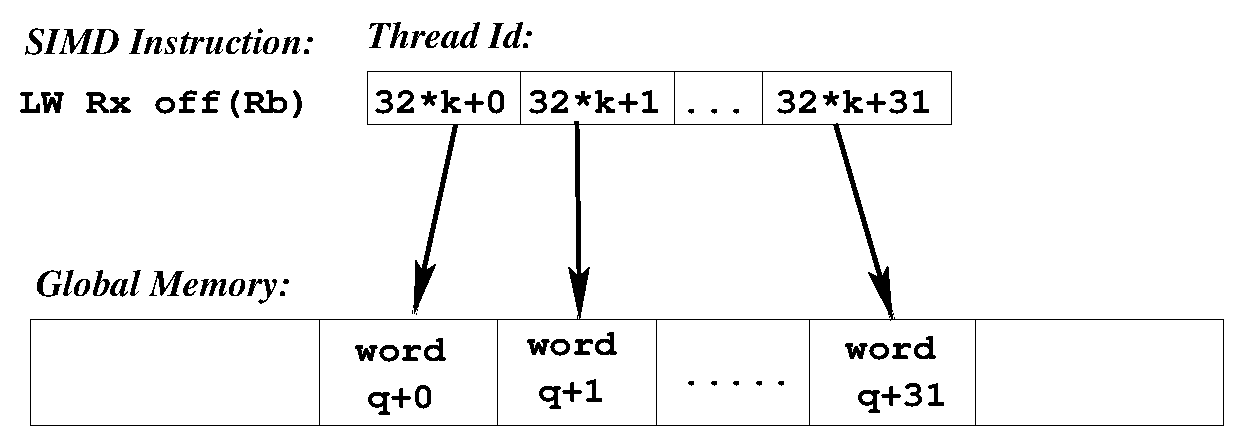
\includegraphics[width=70ex]{Figures/L5/CoalescedGPU}
\caption{Coalesced Access Pattern: the threads executing in lockstep access consecutive global-memory locations in a SIMD load or store instruction.}
\label{fig:coal-gpu}
\end{figure} 

\begin{mydef}[Coalesced Access]\label{coalescedDef}
$\mbox{ }$\\
A read or write access to GPU global memory is said to be
coalesced, if the consecutive threads that execute in lockstep
access consecutive global-memory locations in the corresponding 
SIMD load or store instruction.
\end{mydef}

The definition above and \cref{fig:coal-gpu} introduce the notion
of coalesced access to global memory. This corresponds to a certain 
memory pattern, whose spatial locality is efficiently supported 
by the GPU hardware. In essence if the threads that execute in lockstep 
access consecutive memory locations in their SIMD load or store
instruction, then the GPU memory system will perform the data transfer
in only one memory transaction. Otherwise, if the memory locations 
accessed by the $w$ lockstep-executing threads are spread out in memory,
executing the SIMD load or store instruction may require up to $w$ memory
transactions.  Given that, in practice, common values for $w$ are $16$ and
$32$, optimizing a program to perform coalesced (rather than uncoalesced)
accesses to global memory gives an important (huge) performance boost. 

Luckily, in the case when the array subscript is an affine formula of the 
indices of the enclosing loop nest, then a general technique exists for
optimizing coalesced accesses. The technique relies on changing the 
layout of the corresponding multi-dimensional arrays by means of 
(generalized) transposition. We demonstrate the technique on the 
code example below:

\begin{lstlisting}[mathescape=true]
float A[N,64];
// ... code to fill in array A
float B[N,64];
forall (i=0; i<N; i++) {  // parallel
  float tmpA, tmpB, accum;
  tmpB = A[i,0] * A[i,0];
  B[i,0] = tmpB;
  for(j=1; j<64; j++) { // sequential
    tmpA   = A[i,j];
    accum  = sqrt(tmpB) + tmpA*tmpA;
    B[i,j] = accum;
    tmpB   = accum;
  }
}
\end{lstlisting}\vspace{-2ex}

In the code example, the outermost loop is parallel (why?) and the inner 
loop is sequential (why?). It follows that the CUDA kernel would correspond 
to the body of the outermost loop (which includes the inner loop), and a 
number of (at least) {\tt N} CUDA threads are spawned to execute the kernel.  

Let us analyze what happens when a warp\footnote{
In CUDA terminology, a warp is the group threads that execute 
in lockstep an SIMD instruction. 
}
of threads execute statement {\tt tmpA = A[i,j]} in some fixed iteration 
{\tt j} of the inner loop. Since {\tt i} ranges through thread numbers, 
the values of {\tt i} for the current warp {\tt k} can be written 
as {\tt 32*k+0, 32*k+1, $\ldots$, 32*k+31}. It follows that in the original
program, the SIMD load instruction from array {\tt A} will read the following 
(flattened) words/locations of {\tt A}:
{\tt (32*k+0)*64 + j, (32*k+1)*64 + j, $\ldots$, (32*k+31)*64 + j}.
This corresponds to a strided access in which the stride is {\tt 64} words,
no matter of the value of {\tt j}---i.e., each thread accesses a location 
which is {\tt 64} words apart from the previous thread access. As such
we can expect that our SIMD load instruction will generate {\tt 32} 
independent memory transactions, resulting in terribly inefficient
execution.  Similar thoughts apply to the SIMD instructions executing
the load from {\tt A[i,0]} and the store to {\tt B[i,0]} and {\tt B[i,j]}.

One can optimize the program by changing the layout of the input and result
arrays {\tt A} and {\tt B}, respectively:
\begin{itemize}
    \item[(1)] introduce a new computation before the loop that stores in 
        array {\tt A'} the transposed form of array {\tt A};
    \item[(2)] inside the loop, rewrite the uncolaesced accesses to {\tt A} 
        and {\tt B} into coalesced accesses to {\tt A'} and {\tt B'}---where 
        {\tt B'} is similarly the transpose of {\tt B};
    \item[(3)] introduce a new computation after the loop that transposes
        {\tt B'} into {\tt B}.
\end{itemize} 
Applying the transformation results into the semantically-equivalent program:
\newpage

\begin{lstlisting}[mathescape=true]
float A [N,64];
float A'[64,N];
// ... code to fill in array A
float B [N,64];
float B'[64,N];
A' = transpose(A);
forall (i=0; i<N; i++) {  // parallel
  float tmpA, tmpB, accum;
  tmpB = A'[0,i] * A'[0,i];
  B'[0,i] = tmpB;
  for(j=1; j<64; j++) { // sequential
    tmpA   = A'[j,i];
    accum  = sqrt(tmpB) + tmpA*tmpA;
    B'[j,i]= accum;
    tmpB   = accum;
  }
}
B = transpose(B');
\end{lstlisting}\vspace{-2ex}
Now all the read and write accesses to arrays {\tt A'} and {\tt B'} 
are coalesced. Take for example the read access to {\tt A'[j,i]}.
The current warp {\tt k} will result in the following values of {\tt i}: 
{\tt 32*k+0, 32*k+1, $\ldots$, 32*k+31}. For a fixed {\tt j}, the
flat locations read from {\tt A'[j,i]} by the current warp will be
{\tt j*N + (32*k+0), j*N + (32*k+1), $\ldots$, j*N + (32*k+31)}, 
because the size of the innermost dimension of {\tt A'} is {\tt N}.
It follows that the current warp accesses in the same SIMD
load instruction consecutive memory locations, hence the access is
coalesced. Similar thoughts apply to the read from {\tt A'[0,i]}
and to the write to {\tt B'[0,i]} and {\tt B'[j,i]}.

Note that the original program performs {\tt N*64} reads (from {\tt A}) 
and {\tt N*64} writes (to {\tt B}) to global memory. The transformed
program performs $3\times$ more reads and writes than the original
program, because of the two \lstinline{transpose} operations. 
In spite of this, one is likely to observe that the transformed program
executes much faster than the original one, because it exhibits the kind
of spatial locality (of accesses to {\tt A'} and {\tt B'}) that is efficiently
supported by the GPU hardware.

Next section presents how the \lstinline{transpose} operation can be
efficiently implemented in CUDA, such that it uses only coalesced
(read and write) accesses to global memory.
  
\subsection{Transposition: Block Tiling Optimizes Spatial Locality}
\label{subsec:transp}

In the previous section we have seen how one can transform uncoalesced
accesses to global memory into coalesced ones by means of transposition.
However, this assumes that the \lstinline{transpose} operation itself
can be written only in terms of coalesced accesses to global memory.
This step is nontrivial and is covered in this section. 

We start with the mathematical definition of the {\tt transpose} operator:
given a $r\times c$ matrix {\tt A}---where $r$ and $c$ denotes the number
of rows and columns, respectively---the transpose of {\tt A}, denoted 
{\tt A'} is a $c\times r$ matrix such that {\tt A'[j,i] = A[i,j]}, 
$\forall i\in \{0 \ldots r-1\}$ and $\forall j\in\{0\ldots c-1\}$.
This leads to the following naive code:

\begin{lstlisting}[mathescape=true]
forall (i=0; i<R; i++) {  // parallel
  forall (j=0; j<C; j++) { // parallel
    A'[j,i] = A[i,j];
} }
\end{lstlisting}\vspace{-2ex}

In the naive code, both loops are parallel and the second one
of index {\tt j} iterates faster. It follows that the read access
from {\tt A[i,j]} will be coalesced and the write access to {\tt A'[j,i]}
will be uncoalesced. Intuitively, if {\tt C} is a multiple of $32$, then:
\begin{itemize}
    \item a warp of threads would correspond to the same value of {\tt i} and 
        consecutive values of {\tt j}: {\tt k*32+0, k*32+1, $\ldots$, k*32 + 31},
    \item the flat indices of {\tt A'[j,i]} written by a warp in an SIMD instruction
        will have the form: {\tt (k*32+0)*R + i, (k*32+1)*R + i, $\ldots$, (k*32+31)*R + i}
        which corresponds to a strided access with stride equal to the number of rows 
        {\tt R}, hence the write is not coalesced.
\end{itemize}

We aim to have both accesses to {\tt A} and {\tt A'} in coalesced form. 
The first step is to apply block tiling with a generic tile of size {\tt T}
to both parallel loops. We recall that block tiling corresponds to stripmining
both loops with an inner one that goes with a count {\tt T} and increment one,
followed by interchanging the stripmined loops in the innermost position.
The safety of the interchange is guaranteed by the parallel nature of the
two loops (see \cref{Par-Loop-Interch}). After applying block tiling the
code becomes:\smallskip

\begin{lstlisting}[mathescape=true]
forall (ii=0; ii<R; ii+=T) {  // parallel grid.y
  forall (jj=0; jj<C; jj+=T) { // parallel grid.x
    forall (i=ii; i<min(ii+T,R); i++) {  // parallel block.y
      forall (j=jj; j<min(jj+T,R); j++) {  // parallel block.x
        A'[j,i] = A[i,j];
    } }
} }
\end{lstlisting}

In the code above, the outer two loops of indices {\tt ii} and {\tt jj}
will correspond to the CUDA grid, while the innermost two loops of
indices {\tt i} and {\tt j} will correspond to the CUDA block---i.e.,
we will work with two-dimensional grids of blocks, in which the block
is also two dimensional. Please note that the total size of a block
cannot exceed $1024$ in CUDA, and the size of our CUDA block will be
{\tt T$\times$T} because each inner loop has count {\tt T}. It follows
that {\tt T$^2 \leq$ 1024}, hence valid values of {\tt T} are less than
or equal to {\tt 32}.

We assume for simplicity that {\tt R} and {\tt C} evenly divide {\tt T}.
Let us compute first the indices that are read from and written into
arrays {\tt A} and {\tt A'}, respectively, for a given block 
{\tt [ii,jj]} in the grid.  The innermost two loops have indices
{\tt i = ii+0,$\ldots$,ii+T-1} and {\tt j = jj+0,$\ldots$, jj+T-1},
hence our block will read the slice {\tt A[ii:ii+T, jj:jj+T]}.
By convention the slice excludes the last element, so the size of
the slice is naturally {\tt T$^2$}. We would like to read the slice
in shared memory---we recall that CUDA's ``shared'' memory refers to 
fast scratchpad memory---and figure out from there how to rewrite the
write access to be coalesced. 
%and will write the slice {\tt A'[jj:jj+T, ii:ii+T]}, respectively.
The CPU orchestrating code is:  
\begin{lstlisting}[mathescape=true]
void transposeFloat( float* mat, float* mat_tr, 
                     const unsigned int R, // height 
                     const unsigned int C  // width
) {
  unsigned int dimy = (R + T - 1) / T;
  unsigned int dimx = (C + T - 1) / T;
  dim3 block(T,T,1), grid (dimx, dimy, 1);
  transpose<<< grid, block >>>(mat, mat_tr, R, C);
}
\end{lstlisting}\vspace{-1ex}
and the intermediate code of the CUDA kernel is presented below:\smallskip

\begin{lstlisting}[mathescape=true]
__global__ void transpose(float* A, float* trA, int R, int C) {
  __shared__ float tile[T][T];
  unsigned int tidx = threadIdx.x;
  unsigned int tidy = threadIdx.y;
  unsigned int j = blockIdx.x*T + tidx;
  unsigned int i = blockIdx.y*T + tidy;
  if( j < C && i < R )
    tile[tidy][tidx] = A[i*colsA + j];
  __syncthreads();
  if ( j < C && i < R )
    trA[j*R + i] = tile[tidy][tidx];
}
\end{lstlisting}\vspace{-2ex}
The code above simply spawns a CUDA thread for each of the elements of {\tt A},
then it computes the corresponding indices {\tt i} and {\tt j} for a given thread.
Please note that the iteration space corresponds directly to the input array:
the two-dimensional grid contains $\lceil\frac{R}{T}\rceil\times\lceil\frac{C}{T}\rceil$ 
blocks, each block containing {\tt T$\times$T} elements.
Index {\tt i} is obtained by computing the displacement of the current block
on the {\tt y} axis---i.e., {\tt blockIdx.y*T} to which we add the row number
of the current block---i.e., {\tt threadIdx.y}. Index {\tt j} is computed in a similar way.
The kernel then copies element {\tt A[i,j]} in a {\tt T$\times$T} array, named 
{\tt tile}, which is allocated in shared memory, and finally it reads the same 
element from shared memory and writes it in the transposed position in the 
transposed array. 

So far, we have accomplished nothing, because the access to {\tt trA} is
still uncoalesced; in essence a coalesced access should have a {\tt + tidx} term,
but our access has a {\tt + tidx*R} term which would correspond to a strided 
access to global memory by a stride equal to {\tt R}. This is because we currently
use thread {\tt [tidy,tidx]} to write the local element {\tt tile[tidy][tidx]}
to result array {\tt trA}. 

\enlargethispage{\baselineskip}

The essential step in fixing the uncoalesced access is to use the current thread 
{\tt [tidy,tidx]} to write the ``transposed'' local element in the current block, 
i.e., {\tt tile[tidx][tidy]}. This introduces non-coalesced access to {\tt tile},
which is fine because {\tt tile} is allocated in shared memory and it does not
suffer the penalty of non-coalesced accesses (only global-memory accesses do!).
The global index in {\tt A} corresponding to local element  {\tt tile[tidx][tidy]}
will be {\tt i' = blockIdx.y*T + tidx} and {\tt j' = blockIdx.x*T + tidy},
which will be written in {\tt trA[j',i']}, resulting in coalesced access to
{\tt trA} because {\tt i'} carries the {\tt + tidx} term---i.e., {\tt T}
consecutive threads on the {\tt x} direction will write {\tt T} consecutive 
element locations in memory. The final code is presented below:
\begin{lstlisting}[mathescape=true]
__global__ void transpose(float* A, float* trA, int R, int C) {
  __shared__ float tile[T][T+1];
  unsigned int tidx = threadIdx.x;
  unsigned int tidy = threadIdx.y;
  unsigned int j = blockIdx.x*T + tidx;
  unsigned int i = blockIdx.y*T + tidy;
  if( j < C && i < R )
    tile[tidy][tidx] = A[i*colsA + j];
  __syncthreads();
  unsigned int j' = blockIdx.x*T + tidy;
  unsigned int i' = blockIdx.y*T + tidx;
  if ( j' < C && i' < R )
    trA[j'*R + i'] = tile[tidx][tidy];
}
\end{lstlisting}\vspace{-1ex}

The observant reader has noticed a modification in the declaration of the
shared memory buffer {\tt tile}: previously it was declared as a {\tt T$\times$T}
array, while now it is declared as a {\tt T$\times$(T+1)} array. 
The reason for that is that, in CUDA, the number of shared-memory banks is
a power of two: typically $16$ or $32$. The shared memory does not need to
be accessed in coalesced fashion, but it suffers a significant performance
bottleneck when two threads in the same warp access in an SIMD load or store
instruction two memory locations situated on the same bank. In this case the
two (or multiple) accesses are sequentialized; while the shared-memory transactions
have much smaller latency than global-memory transactions, this bottleneck may
still significantly restrict performance gains.

Assume that in our code we use {\tt T=32} and CUDA shared memory is also 
distributed on $32$ banks. If we declare our {\tt tile} array to be of size
{\tt T$\times$T} then the last read access from {\tt tile[tidx][tidy]} 
would have an entire warp reading different memory locations from the
same memory bank. This is because {\tt tidx} ranges through {\tt 0,$\ldots$,31}
and {\tt tidy} is the same for an entire warp---i.e., with our setting we will
have {\tt tidy} ranging through the warps in a CUDA block. It follows
that an entire warp will access the same shared-memory bank {\tt tidy} 
in the last read from {\tt tile[tidx][tidy]}, and the {\tt 32}
shared-memory transactions of the warp will be sequentialized. 
Luckily, the fix is simple: we make the innermost dimension of our
shared-memory buffer equals to {\tt T+1} rather than {\tt T}, which
will spread the accesses in a warp to different banks. This comes at
the expense of allocating an additional number of {\tt T} shared-memory
locations which will not be utilized.

\subsection{Matrix-Matrix Multiplication: Block Tiling Optimizes Temporal Locality}
\label{subsec:block-mmm}

We turn our attention to how block tiling can optimize temporal locality
of reference. 
We use for demonstration the dense matrix-matrix multiplication 
algorithm.   We start from the naive implementation given below, which
multiplies matrices {\tt A} and {\tt B} whose sizes are {\tt M$\times$U}
and {\tt U$\times$N}, respectively, and results in a matrix {\tt C} of
size {\tt M$\times$N} (i.e., {\tt M} rows and {\tt N} columns):\smallskip

\begin{lstlisting}[mathescape=true]
forall (i=0; i<M; i++) {  // parallel map
  forall (j=0; j<N; j++) {  // parallel map
    float c = 0.0;
    for (k=0; k<U; k++) {    // sequential (reduce o map)
      c += A[i,k] * B[k, j]
    }
    C[i,j] = c;
  } 
}
\end{lstlisting}

One can observe that there is potential to exploit temporal locality:
read access {\tt A[i,k]} is invariant to the second loop of index {\tt j},
and read access {\tt B[k,j]} is invariant to the outermost loop of index 
{\tt i}. As such the program redundantly reads each element of {\tt A}
{\tt N} times, and each element of {\tt B} {\tt M} times. However, in the
current form it is not possible to (fully) exploit the temporal locality 
to arrays {\tt A} and {\tt B}.

We restructure the code by applying block tiling to the two outer 
loops---i.e., we stripmine them, each with a tile equal to {\tt T} 
and we interchanges inwards the stripmined loops of stride one---and 
we also stripmine the innermost loop of index {\tt k}.
This results in the code shown in \cref{fig-mat-mat-mul-c-code}.

\begin{figure}
\begin{lstlisting}[mathescape=true]
forall (ii=0; ii<M; ii+=T) {  // parallel grid.y
  forall (jj=0; jj<N; jj+=T) {  // parallel grid.x
    forall (i=ii; i<min(ii+T,M); i++) { // parallel block.y
      forall (j=jj; j<min(jj+T,M); j++) { // parallel block.x
        float c = 0.0;
        for (kk=0; kk<U; kk+=T) {    // sequential (reduce o map)
          // The loop below reads the following slices:
          // A[ii:ii+T, kk:kk+T] and B[kk:kk+T, jj:jj+T]
          for (k=kk; k<min(kk+T,U); k++) { // sequential
            c += A[i,k] * B[k, j]
        } }
        C[i,j] = c;
    } }
} } 
\end{lstlisting}\vspace{-4ex}
\caption{C-like pseudocode for block-tiled matrix matrix multiplication}
\label{fig-mat-mat-mul-c-code}
\end{figure}

In the restructured code, we reason as before that the two outer loops
correspond to a two-dimensional CUDA grid containing 
$\lceil \frac{M}{T} \rceil \times \lceil \frac{N}{T} \rceil$ two-dimensional
blocks. A CUDA block would correspond to the third and fourth loops of
indices {\tt i} and {\tt j}, thus each block contains $T \times T$ threads.
With the code in this form we turn our attention to the elements that
are accessed in the innermost loop of index {\tt k}. This loop accesses
elements of {\tt A} in the slice {\tt A[ii:ii+T, kk:kk+T]} and elements
of {\tt B} in the slice {\tt B[kk:kk+T, jj:jj+T]}. 

In essence, a given CUDA block of size {\tt T$\times$T}, performs
in some iteration of the {\tt kk} loop a total of {\tt 2$\times$T$^3$} 
accesses to global memory ({\tt T$^3$} to array {\tt A} and {\tt T$^3$} 
to array {\tt B}), but the number of {\em distinct} elements of 
{\tt A} and {\tt B} which are accessed in a block is only {\tt T$^2$}.
We can take advantage by this property by making the threads of a CUDA
block to collectively copy just before the entry into the loop of index
{\tt k} the slices {\tt A[ii:ii+T, kk:kk+T]} and {\tt B[kk:kk+T, jj:jj+T]}
to buffers allocated in shared memory. This would allow the innermost
loop to only access the shared memory buffers instead of global memory.
The resulted CUDA kernel code is shown in \cref{fig-mat-mat-mul-kernel}.

\begin{figure}
\begin{lstlisting}[mathescape=true]
__global__ void MatMatMult( float* A, float* B, float* C
                          , int M, int N, int U) {
  __shared__ float Ash[T][T];
  __shared__ float Bsh[T][T];
  unsigned int tidx = threadIdx.x, tidy = threadIdx.y;
  unsigned int ii = blockIdx.y * T, jj = blockIdx.x * T;
  unsigned int i  = ii + tidy;
  unsigned int j  = jj + tidx;
  float c = 0.0;
  for (int kk=0; kk<U; kk+=T) {    // sequential (reduce o map)
    Ash[i-ii][tidx] = (i < M && kk+tidx < U) ? 
                      A[i*U + (kk+tidx)] : 0.0;
    Bsh[tidy][j-jj] = (j < N && kk+tidy < U) ? 
                      B[(kk+tidy)*N + j] : 0.0;
    __syncthreads();
    #pragma unroll
    for (int k=0; k<T; k++) { // sequential
      c += Ash[i-ii][k] * Bsh[k][j-jj];
    }
    __syncthreads();
  }
  if (i < M && j < N)
    C[i*N + j] = c;
}
\end{lstlisting}\vspace{-4ex}
\caption{CUDA kernel code for block-tiled matrix matrix multiplication}
\label{fig-mat-mat-mul-kernel}
\end{figure}

The CPU orchestrating code that calls the kernel is shown below:
\begin{lstlisting}[mathescape=true]
double MatMatMultFloat( float* A_d, float* B_d, float* C_d, 
                      int M, int N, int U ) {
  unsigned int dimy = (M + T - 1) / T;
  unsigned int dimx = (N + T - 1) / T;
  dim3 block(T,T,1), grid (dimx, dimy, 1);

  unsigned long int elapsed;
  struct timeval t_start,t_end,t_diff;
  gettimeofday(&t_start, NULL);
  MatMatMult<<< grid, block >>>(A_d, B_d, C_d, M, N, U);
  gettimeofday(&t_end, NULL);
  timeval_subtract(&t_diff, &t_end, &t_start);
  elapsed=(t_diff.tv_sec*1e6 + t_diff.tv_usec);
  double flops = 2.0 * M * N * U;
  double gigaFlops=(flops*1.0e-3f) / elapsed;
  return gigaFlops;
}
\end{lstlisting}\vspace{-1ex}
The CPU code measures the kernel runtime, and then computes the performance in
giga floating-point operations per second ($1$ GFlops per sec = $10^9$ 
flops per sec). The number of floating-point operations for matrix-matrix 
multiplication is: {\tt 2$\times$M$\times$N$\times$U} because there
are three nested loops of size {\tt M}, {\tt N}, and {\tt U} which perform
a floating-point addition and a multiplication.  The {\tt elapsed} time
has been computed in microseconds ($1$ microsecond equals $10^{-6}$ seconds).
It follows that the number of giga-flops per second equals the number of
flops divided by the time in microseconds and the result is divided by 
an extra $10^{3}$.

We conclude by remarking that block tiling can be similarly applied
in one dimension or in more dimensions (e.g., three dimensions)---it
all depends on how many loops do we need to tile in order to exploit
temporal locality.  
\begin{lstlisting}[mathescape=true]
forall (i=0; i<M; i++) {  // parallel
    float s = 0, a = A[i];   float a_sq = a * a;
    for (k=0; k<N; k++) {    // sequential
      float a_k = A[k];
      s += sqrt (a_sq - a_k*a_k);
    }
    B[i] = s;
}
\end{lstlisting}\vspace{-1ex}

For example, in the code above the access to {\tt A[k]} is invariant to the
outermost parallel loop, and can be optimized by one-dimensional tiling as below:
\begin{lstlisting}[mathescape=true]
forall (ii=0; ii<M; ii+=T) {  // grid.x
  forall (i=ii; i<min(ii+T,M); i++) { // block.x of size T
    __shared__ float Ash[T];
    float s = 0, a = A[i];
    float a_sq = a * a;
    for (kk=0; kk<N; kk+=T) {  // sequential
      // collectively copy A[kk:kk+T] in Ash[0:T]
      for (k=kk; k<min(kk+T,N); k++) { // sequential
        float a_k = Ash[k-kk];
        s += sqrt (a_sq - a_k*a_k);
      }
    }
    B[i] = s;
  } 
}
\end{lstlisting}\vspace{-1ex}


\subsection{Exercise: Block and Register Tiling for Matrix-Matrix Multiplication}
\label{subsec:block-reg-tiled-mmm}

This section presents the steps by which block and register tiling can
be combined to further optimize the temporal locality of matrix-matrix
multiplication.  We start as before with the naive code:
\begin{lstlisting}[mathescape=true]
forall (i=0; i<M; i++) {  // parallel map
  forall (j=0; j<N; j++) {  // parallel map
    float c = 0.0;
    for (k=0; k<U; k++) {    // sequential (reduce o map)
      c += A[i,k] * B[k, j]
    }
    C[i,j] = c;
  } 
}
\end{lstlisting}\vspace{-1ex}

We then tile the three loops in the following way: 
\begin{itemize}
    \item we stripmine the parallel dimension of index {\tt i} by a tile of
        size {\tt T} and stride {\tt 1};
    \item we double stripmine the second parallel dimension of index {\tt j} by
            a tile of size {\tt T$^2$} and stride {\tt T}, and then by a tile
            of size {\tt T} and stride {\tt 1};
    \item we stripmine the sequential dimension of index {\tt k} by a tile
        of size {\tt T} and stride {\tt 1}. 
\end{itemize}
Since the loops of index {\tt i} and {\tt j} are parallel, we can interchange 
their tiles inwards and distribute them as we desire, and our desire is as follows:
\begin{itemize}
    \item we move the tile of loop {\tt i} innermost and we sequentialize it;
    \item we move the double tiles of the loop of index {\tt j} just inside the 
            original loop of index {\tt k}.
\end{itemize}

\begin{figure}
\begin{lstlisting}[mathescape=true]
unsigned int ii, i, jjj, jj, j, kk, k;
forall (ii = 0; ii < M; ii += T ) {           // parallel grid.y
  forall (jjj = 0; jjj < N; jjj += T*T ) {    // parallel grid.x
    float cs[T][T][T];

    forall(jj=jjj; jj<min(jjj+T*T,N); jj+=T){ // parallel block.y
      forall(j=jj; j<min(jj+T,N); j++) {      // parallel block.x
        for (i=ii; i<min(ii+T,M); i++) {      // sequential
          cs[(jj-jjj)/T][j-jj][i-ii] = 0.0;
    } } }

    for (kk = 0; kk < U; kk += T) {                 // sequential
      // here we will insert a collective copy to shared
      // memory of the slice: A[ii : ii+T, kk : kk+T]
      for (k = kk; k < min(kk+T,U); k++) {          // sequential
        forall (jj=jjj; jj<min(jjj+T*T,N); jj+=T) { // block.y
          forall (j=jj; j<min(jj+T,N); j++) {       // block.x
            float b = B[k,j];                       // hoisted out
            for (i = ii; i < min(ii+T,M); i++) {    // sequential
              // please modify here to read from shared
              //  memory Ash and to scalarize cs
              cs[(jj-jjj)/T][j-jj][i-ii] += A[i,k] * b;
    } } } } }

    forall (jj=jjj; jj<min(jjj+T*T,N); jj+=T) {     // block.y
      forall (j=jj; j<min(jj+T,N); j++) {           // block.x
        for (i = ii; i < min(ii+T, M); i++) {       // sequential
          C[i,j] = cs[(jj-jjj)/T][j-jj][i-ii];
    } } }
}  }
\end{lstlisting}\vspace{-4ex}
\caption{C-like pseudocode for block+register tiled matrix matrix multiplication}
\label{fig-mat-mat-mul-block-reg-c}
\end{figure}

The resulting code is shown in \cref{fig-mat-mat-mul-block-reg-c}: 
\begin{itemize}
    \item the two outer parallel loops of indices {\tt ii} and {\tt jjj} correspond
        to the two-dimensional CUDA grid, which contains 
        $\lceil\frac{M}{T}\rceil\times\lceil\frac{N}{T^2}\rceil$ blocks;
    \item the parallel loops of indices {\tt jj} and {\tt j} correspond to
        the CUDA block, which, as before, has size {\tt T$\times$T};
    \item the loop of index {\tt i} is sequentially executed 
            (part of the kernel code);
    \item we have explicitly distributed the loops of indices {\tt jj}, 
        {\tt j} and {\tt i} across the intialization of {\tt c=0.0},
        the computation of {\tt c} and the update of result matrix {\tt C}.
        This has required to expand scalar {\tt c} with three array dimensions
        all equal with {\tt T}. This step was not shown in the block-tiled
        matrix matrix multiplication because there the distributed loops
        were only the ones forming the CUDA block.  These two dimensions
        of size {\tt T} can be ignored as well in the CUDA code for the
        same reason. However, {\tt c} needs to be expanded with a dimension
        of size {\tt T} in the CUDA code due to the distribution of the loop
        of index {\tt i}, which is sequentialized in the block+register tiled
        version of the code;
    \item please notice that the read from global memory {\tt B[k,j]} has
        been hoisted outside the innermost loop of index {\tt i} since it
        is invariant to it;
    \item each thread now computes {\tt T} elements on a column of the result array: 
        the local thread of block index {\tt threadIdx.y = (jj-jjj)/T} and 
        {\tt threadIdx.y = j-jj} in some block {\tt blockIdx.y = ii} and 
        {\tt blockIdx.x = jjj]} computes the elements {\tt C[ii:ii+T,j]}
        by sequentially iterating at most {\tt T} times through the
        loop of index {\tt i} in the last loop nest.
\end{itemize}

Your task is to implement the CUDA code for the block+register tiled
matrix matrix multiplication---including the CPU orchestration code 
and the kernel code---specialized for the case when {\tt T=16}. 
The following details are probably important:
\begin{itemize}
    \item make the threads of the block to collectively copy the slice
        {\tt A[ii:ii+T, kk:kk+T]} into shared memory just inside the
        loop of index {\tt kk};
    \item Insert the necessary synchronization
        and replace the read from {\tt A[i,k]} in the innermost loop 
        body with a read access from shared memory;
    \item semantically, each thread should work with its own (private) 
        array {\tt cs} of size {\tt T}; you do not necessarily need
        to scalarize this array since the CUDA compiler might do it
        for you. However, if in doubt you may scalarized the {\tt cs} 
        array for {\tt T=16}---please consult \cref{subsec:strip-tiling} 
        and \cref{fig-unroll-jam} for inspiration.
    \item please make sure that all the loops of indices {\tt i}
        and {\tt k} are normalized---i.e., they go from {\tt 0}
        to {\tt T} with a stride of {\tt 1}---and the loop of index
        {\tt i} is unrolled (specified with {\tt \#pragma unroll} before it),
        but the loop of index {\tt k} is not unrolled! 
\end{itemize}

Please report the GFlops per second achieved by your implementation,
and compare the performance with the provided block-tiled version.
Please also answer what is the degree of temporal reuse for the
matrix {\tt A} and for the matrix {\tt B} in your implementation,
i.e., ``A read from {\tt A} and {\tt B} stored in global memory is 
amortized by how many shared-memory or register accesses?''

\newpage
%% Bibliography
\bibliography{pmph.bib}

\end{document}

%%% Local Variables:
%%% mode: latex
%%% TeX-master: t
%%% End:
